\documentclass[a4paper,oneside]{report}
\usepackage[fontsize=13pt]{scrextend}      % Cỡ chữ 13 pt (như \changefontsizes{13pt} của mẫu SoICT)
% Toàn bộ định dạng nằm trong hust-datn.sty: lề, font, giãn dòng, đầu trang, tiêu đề, chú thích
% hình/bảng, bảng, mục lục, trích dẫn IEEE. Từ 07/11/2026 định dạng theo mẫu LaTeX ĐATN SoICT
% (thư mục Do_An_Latex_SoiCT); trang bìa giữ theo định dạng riêng của sinh viên.
% Bản trước khi chuyển sang mẫu SoICT: backup/2026-11-07_truoc-mau-soict/.
\usepackage{hust-datn}
\makeindex

% Thông tin dùng chung
\newcommand{\tendetai}{Xây dựng hệ thống quản lý tín chỉ các-bon trên blockchain}
\newcommand{\thoigiannop}{1/2027}   % Tháng/năm nộp quyển, in ở cuối trang bìa

\usepackage[unicode,hidelinks,bookmarksnumbered]{hyperref}   % luôn nạp sau cùng
% Cho phép ngắt dòng URL dài trong danh mục tài liệu tham khảo tại dấu gạch nối, dấu chấm
\expandafter\def\expandafter\UrlBreaks\expandafter{\UrlBreaks\do\-\do\.\do\/}

\begin{document}
\bstctlcite{BSTcontrol}   % in đầy đủ tên tác giả lặp lại trong TLTK (không dùng "——"), xem References.bib

% ================= 1. BÌA TRƯỚC (giữ nguyên định dạng của sinh viên) =================
\newgeometry{top=2cm,bottom=2cm,left=2.5cm,right=2cm}
\begin{titlepage}
    \setstretch{1}
    \setlength{\parskip}{0pt}
    \centering

    {\fontsize{14}{17}\selectfont\bfseries
        ĐẠI HỌC BÁCH KHOA HÀ NỘI\\
        KHOA TOÁN – TIN\par}

    \vspace{6.2cm}

    {\fontsize{18}{22}\selectfont\bfseries ĐỒ ÁN TỐT NGHIỆP\par}

    \vspace{22pt}

    % Tên đề tài phải khớp đúng với tên đã đăng ký trong phiếu giao nhiệm vụ
    {\fontsize{14}{17}\selectfont\bfseries \tendetai\par}

    \vspace{18pt}

    {\fontsize{14}{20}\selectfont
        \textbf{NGUYỄN CẢNH DUY}\\
        Email: Duy.NC227174@sis.hust.edu.vn\\
        Mã sinh viên: 20227174\\
        \textbf{Chuyên ngành Hệ thống thông tin quản lý}\par}

    \vspace{2.2cm}

    {\fontsize{13}{15.6}\selectfont
    \noindent\hspace*{0.6cm}%
    \makebox[5.3cm][l]{\textbf{Giảng viên hướng dẫn:}}%
    \makebox[5.8cm][l]{PGS.TS Lê Chí Ngọc}%
    \raisebox{-4pt}[0pt][0pt]{%
        \parbox[t]{3.5cm}{%
            \rule{3.5cm}{0.5pt}\\[-3pt]
            \hspace*{0.1cm}{\fontsize{10}{12}\selectfont Chữ ký của GVHD}}}%
    \par}

    \vfill

    {\fontsize{13}{15.6}\selectfont\bfseries HÀ NỘI, \thoigiannop\par}
\end{titlepage}
\restoregeometry

% ================= PHẦN ĐẦU: đánh số La Mã, chỉ có số trang ở chân trang =================
\pagenumbering{roman}
\pagestyle{plain}

% ================= 2. ĐỀ TÀI TỐT NGHIỆP / NHẬN XÉT CỦA GIẢNG VIÊN HƯỚNG DẪN =================
% Mẫu SoICT (0_1_De_tai_TN.tex): trang "ĐỀ TÀI TỐT NGHIỆP" có chữ ký GVHD, biểu mẫu theo quy định
% của Khoa. Hướng dẫn của Khoa Toán – Tin (02/04/2025, mục IV.B): "Nhận xét của Giảng viên hướng dẫn
% (phải có chữ ký của Giảng viên hướng dẫn)". Khi có bản scan, đặt file NhanXetGVHD.pdf cùng thư mục.
% [VIẾT SAU] Trang nhận xét GVHD: chèn bản scan khi có — bỏ dấu % ở các dòng dưới để khôi phục.
% \chentrangscan{NhanXetGVHD.pdf}{Nhận xét của giảng viên hướng dẫn}
%     {Chèn bản scan nhận xét có chữ ký của giảng viên hướng dẫn (file NhanXetGVHD.pdf).}

% ================= 3. PHIẾU BÁO CÁO TIẾN ĐỘ ĐỒ ÁN =================
% Phiếu in từ hệ thống số hóa của Khoa (fami.hust.edu.vn/sohoa), đóng vào quyển.
% [VIẾT SAU] Phiếu báo cáo tiến độ: chèn bản scan khi có — bỏ dấu % ở các dòng dưới để khôi phục.
% \chentrangscan{PhieuTienDo.pdf}{Phiếu báo cáo tiến độ đồ án}
%     {Chèn phiếu báo cáo tiến độ in từ hệ thống số hóa (file PhieuTienDo.pdf).}

% ================= 4. LỜI CẢM ƠN + TÓM TẮT (CÙNG 1 TRANG, SINH VIÊN KÝ) =================
% Theo hướng dẫn của Khoa: "Lời cảm ơn" và "Tóm tắt đồ án" trình bày trong 1 trang, sinh viên ký
% và ghi rõ họ tên. Nội dung tóm tắt theo mẫu SoICT (0_3_Tom_tat_noi_dung.tex).
% [VIẾT SAU] Lời cảm ơn và tóm tắt đồ án chưa viết — bỏ dấu % ở các dòng dưới để khôi phục.
% \clearpage
% \begin{center}\vspace*{18pt}\textbf{LỜI CẢM ƠN}\end{center}
% % Ngắn gọn, khoảng 100–150 từ, tránh từ sáo rỗng.
% [Lời cảm ơn]
%
% \begin{center}\vspace{12pt}\textbf{TÓM TẮT NỘI DUNG ĐỒ ÁN}\end{center}
% % Tối đa khoảng 300 chữ, viết thành đoạn văn, không gạch đầu dòng. Theo thứ tự: (i) vấn đề cần
% % giải quyết và hạn chế của các hướng tiếp cận hiện có; (ii) hướng tiếp cận của đồ án và lý do;
% % (iii) tổng quan giải pháp, công cụ sử dụng; (iv) đóng góp chính, kết quả đạt được, tính thực tế,
% % hướng phát triển; kiến thức và kỹ năng đạt được.
% [Tóm tắt nội dung đồ án]
%
% \khoichuky{Sinh viên thực hiện}
%
% % ABSTRACT: không bắt buộc (mẫu SoICT). Nếu viết thì phải đủ nội dung như bản tiếng Việt.
% % \clearpage
% % \begin{center}\vspace*{18pt}\textbf{ABSTRACT}\end{center}
% % [Abstract]

% ================= 5. MỤC LỤC VÀ CÁC DANH MỤC =================
\tableofcontents

\clearpage
\phantomsection
\addcontentsline{toc}{chapter}{DANH MỤC HÌNH VẼ}
\listoffigures

\clearpage
\phantomsection
\addcontentsline{toc}{chapter}{DANH MỤC BẢNG BIỂU}
\listoftables

% Danh mục ký hiệu: bắt buộc theo hướng dẫn của Khoa (mẫu SoICT gọi là "Danh mục từ viết tắt").
% Xếp theo thứ tự chữ cái, mỗi chữ viết tắt chỉ giải thích một lần. Không đưa các mã tự đặt trong
% bài (VĐ-1..5, NC-01..10) vì chúng đã được giải thích ngay trong Chương 1.
\chapter*{Danh mục ký hiệu}
\label{chap:viettat}
\phantomsection
\addcontentsline{toc}{chapter}{DANH MỤC KÝ HIỆU}
\markboth{DANH MỤC KÝ HIỆU}{}
% [RÚT GỌN 07/11/2026] AFOLU, CCC, DPG, EVM, FCPF, ICVCM, LoA, OMGE, VNX không còn dùng trong bản rút gọn
% của Chương 1 — bỏ dấu % khi chương nào dùng lại.
\begin{longtable}{@{}p{2.4cm}p{5.4cm}p{6.3cm}@{}}
\toprule
\textbf{Viết tắt} & \textbf{Tên tiếng Anh} & \textbf{Tên tiếng Việt} \\
\midrule
\endhead
\bottomrule
\endfoot
A6.4ER & Article 6.4 Emission Reduction           & Đơn vị giảm phát thải theo Điều 6.4 Thỏa thuận Paris \\
AEF    & Agreed Electronic Format                  & Định dạng điện tử thỏa thuận \\
% AFOLU  & Agriculture, Forestry and Other Land Use  & Nông nghiệp, lâm nghiệp và sử dụng đất khác \\
API    & Application Programming Interface         & Giao diện lập trình ứng dụng \\
% CCC    & Climate Change Center (Korea)             & Trung tâm biến đổi khí hậu Hàn Quốc \\
% CBAM   & Carbon Border Adjustment Mechanism        & Cơ chế điều chỉnh biên giới các-bon \\
CDM    & Clean Development Mechanism               & Cơ chế phát triển sạch \\
% CDOP   & Carbon Data Open Protocol                 & Giao thức mở dữ liệu các-bon \\
% [VIẾT SAU] CBAM, CSDL, dApp, DeFi, IPFS, PoS, PoW chỉ dùng ở các chương đang để trong chú thích — bỏ dấu % khi khôi phục.
% CSDL   & Database                                  & Cơ sở dữ liệu \\
DAG    & Directed Acyclic Graph                    & Đồ thị có hướng không chu trình \\
% dApp   & Decentralized Application                 & Ứng dụng phi tập trung \\
% DeFi   & Decentralized Finance                     & Tài chính phi tập trung \\
% DPG    & Digital Public Good                       & Hàng hóa công kỹ thuật số \\
ERC    & Ethereum Request for Comments             & Chuẩn kỹ thuật của Ethereum \\
ERPA   & Emission Reductions Payment Agreement     & Thỏa thuận chi trả giảm phát thải \\
% EVM    & Ethereum Virtual Machine                  & Máy ảo Ethereum \\
% FCPF   & Forest Carbon Partnership Facility        & Quỹ đối tác các-bon lâm nghiệp \\
GHG    & Greenhouse Gas                            & Khí nhà kính \\
HNX    & Hanoi Stock Exchange                      & Sở Giao dịch Chứng khoán Hà Nội \\
% ICVCM  & Integrity Council for the Voluntary Carbon Market & Hội đồng liêm chính thị trường các-bon tự nguyện \\
IoT    & Internet of Things                        & Internet vạn vật \\
ISO    & International Organization for Standardization & Tổ chức tiêu chuẩn hóa quốc tế \\
% IPFS   & InterPlanetary File System                & Hệ thống lưu trữ tệp phi tập trung \\
ITMO   & Internationally Transferred Mitigation Outcome & Kết quả giảm nhẹ được chuyển giao quốc tế \\
% LoA    & Letter of Authorization                   & Thư ủy quyền \\
MRV    & Measurement, Reporting and Verification   & Đo đạc, báo cáo, thẩm định \\
NDC    & Nationally Determined Contribution        & Đóng góp do quốc gia tự quyết định \\
NFT    & Non-Fungible Token                        & Token không thể thay thế \\
% OMGE   & Overall Mitigation in Global Emissions    & Giảm nhẹ tổng thể phát thải toàn cầu \\
PACM   & Paris Agreement Crediting Mechanism       & Cơ chế tín chỉ theo Điều 6.4 Thỏa thuận Paris \\
PDD    & Project Design Document                   & Tài liệu thiết kế dự án \\
% PoS    & Proof of Stake                            & Bằng chứng cổ phần \\
% PoW    & Proof of Work                             & Bằng chứng công việc \\
REC    & Renewable Energy Certificate              & Chứng chỉ năng lượng tái tạo \\
tCO\textsubscript{2}e & Tonne of CO\textsubscript{2} equivalent & Tấn CO\textsubscript{2} tương đương \\
UNDP   & United Nations Development Programme      & Chương trình phát triển Liên hợp quốc \\
VCS    & Verified Carbon Standard                  & Tiêu chuẩn các-bon được xác minh của Verra \\
VCU    & Verified Carbon Unit                      & Đơn vị các-bon được xác minh \\
% VNX    & Vietnam Exchange                          & Sở Giao dịch Chứng khoán Việt Nam \\
VSDC   & Vietnam Securities Depository and Clearing Corporation & Tổng công ty Lưu ký và Bù trừ Chứng khoán Việt Nam \\
VVB    & Validation and Verification Body          & Bên thẩm định độc lập \\
\end{longtable}

% Danh mục thuật ngữ (mẫu SoICT, 0_6_Thuat_ngu.tex): chỉ giải thích các thuật ngữ khó hiểu, ít gặp
% ngoài chuyên ngành. Thuật ngữ phổ biến (blockchain, token, API, dashboard, testnet, use case...)
% không đưa vào. Thêm dòng khi chương sau dùng thuật ngữ mới khó hiểu.
\chapter*{Danh mục thuật ngữ}
\phantomsection
\addcontentsline{toc}{chapter}{DANH MỤC THUẬT NGỮ}
\markboth{DANH MỤC THUẬT NGỮ}{}
\begin{longtable}{@{}p{4.2cm}p{9.9cm}@{}}
\toprule
\textbf{Thuật ngữ} & \textbf{Ý nghĩa} \\
\midrule
\endhead
\bottomrule
\endfoot
Additionality   & Tính bổ sung: lượng giảm phát thải sẽ không xảy ra nếu không có dự án \\
Audit trail     & Dấu vết kiểm tra: chuỗi bản ghi cho phép truy lại ai đã làm gì, khi nào \\
Baseline        & Đường phát thải cơ sở: lượng phát thải giả định nếu không có dự án \\
Burn            & Đốt token, tức loại token khỏi lưu thông vĩnh viễn \\
Corresponding adjustment & Điều chỉnh tương ứng: quốc gia chuyển giao trừ lượng giảm phát thải đã bán ra khỏi kết quả thực hiện NDC của mình \\
Credit block    & Khối tín chỉ, gồm một dãy số sê-ri liên tiếp \\
Double counting & Tính toán kép: một lượng giảm phát thải được tính nhiều lần, gồm phát hành kép, sử dụng kép và tuyên bố kép \\
Mint            & Phát hành, tức tạo mới token trên blockchain \\
Pool            & Smart contract nhận NFT của nhiều lô và trả lại token có thể thay thế \\
Pooled buffer account & Tài khoản dự phòng chung của Verra, giữ lại một phần tín chỉ để bù cho rủi ro đảo ngược \\
Reentrancy      & Lỗ hổng cho phép gọi lại hàm của smart contract trước khi lần gọi trước kết thúc \\
Retirement      & Hủy tín chỉ: dùng tín chỉ để bù trừ phát thải và loại tín chỉ khỏi lưu thông \\
Reversal        & Đảo ngược: lượng các-bon đã lưu giữ (ví dụ trong rừng) bị phát thải trở lại \\
Serverless      & Kiến trúc chạy mã theo từng hàm trên nền tảng đám mây, không cần tự quản lý máy chủ \\
Vintage         & Năm xảy ra lượng giảm phát thải ghi trên tín chỉ \\
\end{longtable}

% ================= NỘI DUNG CHÍNH =================
% Theo mẫu SoICT, chương 1 "Giới thiệu đề tài" và chương 2 "Khảo sát và phân tích yêu cầu" được
% gộp thành Chương 1 của báo cáo này. Các chương sau tương ứng với chương 3–6 của mẫu.
% Mỗi chương có đoạn tổng quan ở đầu và đoạn kết chương ở cuối (định dạng Normal, không tiêu đề).
\clearpage
\pagenumbering{arabic}
\pagestyle{noidung}

% Chương 1 = mẫu SoICT chương 1 + chương 2.
% ============================================================
% CHƯƠNG 1 — GIỚI THIỆU VÀ KHẢO SÁT BÀI TOÁN
% Viết lại ngày 07/11/2026 theo mẫu ĐATN SoICT (Do_An_Latex_SoiCT): chương 1 "Giới thiệu đề tài"
% (Đặt vấn đề, Mục tiêu và phạm vi, Định hướng giải pháp, Bố cục) và chương 2 "Khảo sát và phân tích
% yêu cầu" (Khảo sát hiện trạng, Tổng quan chức năng, Đặc tả chức năng, Yêu cầu phi chức năng)
% gộp thành một chương.
% Bản trước khi viết lại: backup/2026-11-07_truoc-mau-soict/Chap1.tex
%
% Quy ước văn phong (theo mẫu SoICT và góp ý của GVHD về dấu hiệu văn bản do AI viết):
%   - viết thành đoạn văn có liên kết, mỗi đoạn một ý chính; hạn chế gạch đầu dòng, khi cần liệt kê
%     thì dùng (i), (ii), (iii) trong câu;
%   - câu chủ động, chủ ngữ là chủ thể thật (đồ án, hệ thống, smart contract, Bộ, Verra, HNX...);
%     hạn chế xưng "em", "tôi"; chỉ dùng "tác giả" ở đoạn kết chương và ở vài đoạn nói về cách
%     sinh viên tự làm (phương pháp khảo sát); hạn chế "được", "bị" và chủ ngữ phiếm chỉ;
%   - mục con dùng \subsection* (không đánh số, không vào mục lục), không \ref tới nhãn mục con;
%   - giữ thuật ngữ CNTT bằng tiếng Anh (blockchain, smart contract, token, pool, on-chain, off-chain,
%     API, dashboard...), thuật ngữ dịch thì ghi kèm tiếng Anh ở lần đầu; xem bảng thuật ngữ ở main.tex.
% [BẢN NHÁP] Sinh viên đọc lại và sửa theo văn phong của mình.
% [VIẾT SAU] = phần chưa làm, đang để trong chú thích.
% Trích dẫn kiểu IEEE, in ra dạng [2][3] (cấu hình trong hust-datn.sty); mỗi ý thường chỉ cite 1–2 nguồn
% quan trọng nhất, viết \cite{a,b}, đặt ~\cite trước dấu câu.
% ============================================================

\chapter{GIỚI THIỆU VÀ KHẢO SÁT BÀI TOÁN}
\label{chap:khaosat}
\label{chap:gioithieu}
% ============================================================
% FIGURES_CHAP1.TEX — Hình tự vẽ (TikZ) cho Chương 1
% Mỗi hình là một lệnh, gọi đúng chỗ trong Chap1.tex:
%   \HinhDieuSau  \HinhMRV  \HinhVaccargiu  \HinhToucan  \HinhKienTruc
% Các hình được vẽ vừa bề rộng vùng chữ (15 cm), không cần thu nhỏ.
% Preamble main.tex cần:
%   \usepackage{tikz}
%   \usetikzlibrary{shapes.geometric,arrows.meta,positioning,calc}
% Nguồn gốc hình (07/11/2026): theo sinh viên, tất cả hình vẽ đều do Claude tạo. Năm hình đầu (DieuSau,
% MRV, Vaccargiu, Toucan, KienTruc) tạo ngày 20/10/2026; HinhMoHinhToChuc tạo ngày 04/11/2026.
% ============================================================

\tikzset{
    hop/.style      = {draw, rounded corners=3pt, align=center,
                       inner sep=3pt, font=\small},
    muiten/.style   = {-{Stealth[length=6pt]}, thick},
    ghichu/.style   = {font=\footnotesize\itshape, text=black!65, align=center},
}

% ------------------------------------------------------------
% HÌNH: Điều 6.2 và Điều 6.4 — đặt sau Bảng so sánh Điều 6
% ------------------------------------------------------------
\newcommand{\HinhDieuSau}{%
\begin{figure}[htbp]
\centering
\begin{tikzpicture}
    % Tiêu đề hai cột và đường phân cách
    \node[font=\bfseries] at (3.4, 0) {Điều 6.2 (song phương)};
    \node[font=\bfseries] at (11.0, 0) {Điều 6.4 (tập trung – PACM)};
    \draw[thick, black!30] (7.3, 0.3) -- (7.3, -7.0);

    % ---- Điều 6.2 ----
    \node[hop, fill=blue!10, minimum width=3.0cm, minimum height=1.1cm]
        (A) at (1.7, -1.3) {\textbf{Quốc gia A}\\(bán ITMOs)};
    \node[hop, fill=blue!10, minimum width=3.0cm, minimum height=1.1cm]
        (B) at (1.7, -4.1) {\textbf{Quốc gia B}\\(mua ITMOs)};
    \node[draw, diamond, aspect=1.8, fill=yellow!25, font=\small,
          inner sep=1pt] (I) at (5.3, -2.8) {ITMOs};
    \draw[muiten] (A.east) -| node[ghichu, pos=0.25, above] {bán} (I.north);
    \draw[muiten] (I.south) |- node[ghichu, pos=0.75, above] {chuyển giao} (B.east);
    \node[hop, fill=red!8, text width=6.2cm, font=\footnotesize]
        (CA) at (3.4, -6.4)
        {\textbf{Điều chỉnh tương ứng:}\\
         Quốc gia A cộng thêm phát thải vào sổ quốc gia;\\
         Quốc gia B được trừ lượng phát thải tương ứng};
    \draw[muiten, dashed, red!60] (B.south) -- (B.south |- CA.north);

    % ---- Điều 6.4 ----
    \node[hop, fill=green!12, minimum width=3.2cm, minimum height=0.9cm]
        (P) at (10.2, -1.2) {Nhà phát triển dự án};
    \node[hop, fill=orange!15, minimum width=3.2cm, minimum height=0.9cm]
        (S) at (10.2, -2.7) {Cơ quan giám sát};
    \node[draw, diamond, aspect=1.8, fill=yellow!25, font=\small,
          inner sep=1pt] (E) at (10.2, -4.3) {A6.4ERs};
    \node[hop, fill=green!12, minimum width=3.2cm, minimum height=0.9cm]
        (U) at (10.2, -5.9) {Người mua / bù trừ};
    \draw[muiten] (P) -- node[ghichu, right] {đăng ký} (S);
    \draw[muiten] (S) -- node[ghichu, left] {cấp} (E);
    \draw[muiten] (E) -- node[ghichu, right] {giao dịch} (U);
    % Khoản trích 5%/2% áp dụng tại thời điểm cấp (quyết định 3/CMA.3), không phải mỗi giao dịch
    \node[hop, fill=red!8, text width=2.3cm, font=\footnotesize]
        (F) at (13.7, -3.5) {Trích khi cấp:\\5\% Quỹ thích ứng\\$\geq$2\% hủy (OMGE)};
    \coordinate (SE) at ($(S.south)!0.5!(E.north)$);
    \draw[muiten, red!60] (SE) -- (SE -| F.west);
\end{tikzpicture}
\caption[Cơ chế hoạt động của Điều 6.2 và Điều 6.4 Thỏa thuận Paris]%
{Cơ chế hoạt động của Điều 6.2 và Điều 6.4 Thỏa thuận Paris~\cite{unfccc2022cma3} \hinhtao[Claude]{20/10/2026}}
\label{fig:dieu6}
\end{figure}}

% ------------------------------------------------------------
% HÌNH: Vòng đời tín chỉ và ISO 14064 — đặt sau Bảng ISO 14064
% ------------------------------------------------------------
\newcommand{\HinhMRV}{%
\begin{figure}[htbp]
\centering
\begin{tikzpicture}[
    buoc/.style = {draw, rounded corners=4pt, align=center,
                   text width=3.4cm, minimum height=1.5cm, font=\small},
]
    % Hàng 1: trái -> phải
    \node[buoc, fill=blue!12]   (s1) at (2.0, 0)
        {\textbf{1. Thiết kế dự án}\\{\footnotesize\itshape PDD – ISO 14064-2}};
    \node[buoc, fill=teal!15]   (s2) at (7.4, 0)
        {\textbf{2. Thẩm định}\\{\footnotesize\itshape VVB – ISO 14064-3}};
    \node[buoc, fill=green!15]  (s3) at (12.8, 0)
        {\textbf{3. Giám sát}\\{\footnotesize\itshape dữ liệu hoạt động}};
    % Hàng 2: phải -> trái
    \node[buoc, fill=yellow!22] (s4) at (12.8, -2.6)
        {\textbf{4. Xác minh}\\{\footnotesize\itshape VVB – ISO 14064-3}};
    \node[buoc, fill=orange!20] (s5) at (7.4, -2.6)
        {\textbf{5. Phát hành}\\{\footnotesize\itshape trừ tài khoản đệm}};
    \node[buoc, fill=red!12]    (s6) at (2.0, -2.6)
        {\textbf{6. Giao dịch \& hủy}\\{\footnotesize\itshape hủy vĩnh viễn (retire)}};

    \draw[muiten] (s1) -- (s2);
    \draw[muiten] (s2) -- (s3);
    \draw[muiten] (s3) -- (s4);
    \draw[muiten] (s4) -- (s5);
    \draw[muiten] (s5) -- (s6);
\end{tikzpicture}
\caption[Vòng đời tín chỉ các-bon và các phần tương ứng của tiêu chuẩn ISO 14064]%
{Vòng đời tín chỉ các-bon và các phần tương ứng của tiêu chuẩn ISO 14064~\cite{iso14064-2,iso14064-3} \hinhtao[Claude]{20/10/2026}}
\label{fig:mrv}
\end{figure}}

% ------------------------------------------------------------
% HÌNH: Kiến trúc 4 lớp của Vaccargiu — đặt sau danh sách 4 lớp (Chương 2, mục \ref{sec:dmrv})
% ------------------------------------------------------------
\newcommand{\HinhVaccargiu}{%
\begin{figure}[htbp]
\centering
\begin{tikzpicture}[
    lop/.style = {draw, rounded corners=5pt, align=center,
                  text width=9.0cm, minimum height=1.3cm, font=\small},
]
    \node[lop, fill=orange!15] (l4) at (4.8, 5.4)
        {\textbf{Lớp 4: Blockchain và chứng nhận}\\
         {\footnotesize Hyperledger Fabric, smart contract tạo và đăng ký tín chỉ}};
    \node[lop, fill=yellow!18] (l3) at (4.8, 3.6)
        {\textbf{Lớp 3: Tổng hợp dữ liệu tại biên}\\
         {\footnotesize tổng hợp theo phút, gom thành lô 5 phút để ghi lên chuỗi}};
    \node[lop, fill=blue!10]   (l2) at (4.8, 1.8)
        {\textbf{Lớp 2: Thu thập dữ liệu}\\
         {\footnotesize cổng nối nhận luồng dữ liệu thời gian thực}};
    \node[lop, fill=green!13]  (l1) at (4.8, 0)
        {\textbf{Lớp 1: Cảm biến vật lý}\\
         {\footnotesize 8 đồng hồ đo thông minh 3 pha (24 pha điện)}};

    \draw[muiten] (l1) -- (l2);
    \draw[muiten] (l2) -- (l3);
    \draw[muiten] (l3) -- (l4);

    % Chú thích bên phải: tần suất / dạng dữ liệu
    \node[ghichu, anchor=west, text width=4.3cm] at (10.2, 5.4) {288 lần ghi / ngày};
    \node[ghichu, anchor=west, text width=4.3cm] at (10.2, 3.6) {1.440 bản ghi / ngày};
    \node[ghichu, anchor=west, text width=4.3cm] at (10.2, 1.8) {luồng dữ liệu liên tục};
    \node[ghichu, anchor=west, text width=4.3cm] at (10.2, 0)   {1–2 giây / lần đo};
\end{tikzpicture}
\caption[Kiến trúc 4 lớp của hệ thống chứng nhận tín chỉ các-bon dựa trên IoT và blockchain]%
{Kiến trúc 4 lớp của hệ thống chứng nhận tín chỉ các-bon dựa trên IoT và blockchain~\cite{vaccargiu2026blockchain} \hinhtao[Claude]{20/10/2026}}
\label{fig:vaccargiu}
\end{figure}}

% ------------------------------------------------------------
% HÌNH: Luồng token Toucan — đặt sau danh sách các bước Toucan (Chương 2, mục \ref{sec:token})
% Theo tài liệu Toucan: Batch NFT là ERC-721, TCO2 là ERC-20 (mỗi dự án–vintage một hợp đồng),
% retire() đốt TCO2; cầu nối Verra đã ngừng hoạt động.
% ------------------------------------------------------------
\newcommand{\HinhToucan}{%
\begin{figure}[htbp]
\centering
\begin{tikzpicture}[
    tok/.style = {draw, rounded corners=4pt, align=center,
                  text width=2.2cm, minimum height=1.3cm, font=\small},
]
    \node[tok, fill=blue!12]   (v) at (1.2, 0)    {\textbf{Verra}\\VCUs};
    \node[tok, fill=teal!15]   (b) at (4.9, 0)    {\textbf{Batch NFT}\\ERC-721};
    \node[tok, fill=teal!25]   (t) at (8.6, 0)    {\textbf{TCO2}\\ERC-20};
    \node[tok, fill=green!15]  (p) at (12.6, 0)   {\textbf{BCT / NCT}\\ERC-20};
    \node[tok, fill=red!12]    (r) at (8.6, -2.8) {\textbf{Hủy}\\burn TCO2};
    \node[tok, fill=yellow!20, text width=2.6cm] (c) at (12.6, -2.8) {\textbf{Chứng nhận}\\hủy (NFT)};

    \draw[muiten] (v) -- node[above, font=\scriptsize] {cầu nối}  (b);
    \draw[muiten] (b) -- node[above, font=\scriptsize] {chia nhỏ} (t);
    \draw[muiten] ([yshift=3mm]t.east) -- node[above, font=\scriptsize\ttfamily] {deposit} ([yshift=3mm]p.west);
    \draw[muiten] ([yshift=-3mm]p.west) -- node[below, font=\scriptsize\ttfamily] {redeem} ([yshift=-3mm]t.east);
    \draw[muiten] (t) -- node[left, font=\scriptsize\ttfamily] {retire()} (r);
    \draw[muiten] (r) -- (c);

    \node[ghichu, text width=2.8cm] at (1.2, -1.5) {VCU được hủy trên\\Verra, ghi mã lô};
    \node[ghichu, text width=2.8cm] at (4.9, -1.5) {Toucan duyệt\\số sê-ri};
    \node[ghichu, text width=3.0cm] at (12.6, -1.5) {1 token = 1 tCO$_2$e};
\end{tikzpicture}
\caption[Luồng token hóa và hủy tín chỉ các-bon qua Toucan Protocol]%
{Luồng token hóa và hủy tín chỉ các-bon qua Toucan Protocol (cầu nối Verra hiện đã ngừng hoạt động)~\cite{toucan2025docs} \hinhtao[Claude]{20/10/2026}}
\label{fig:toucan}
\end{figure}}

% ------------------------------------------------------------
% HÌNH: Kiến trúc tổng thể đề xuất — đặt cuối mục \ref{sec:kientruc} (Chương 3)
% Đây là thiết kế của đồ án nên không trích nguồn. Ô nét đứt = ngoài phạm vi cài đặt.
% ------------------------------------------------------------
\newcommand{\HinhKienTruc}{%
\begin{figure}[htbp]
\centering
\begin{tikzpicture}[
    tp/.style = {draw, rounded corners=3pt, align=center, fill=white,
                 text width=3.0cm, minimum height=1.0cm, font=\footnotesize},
    lp/.style = {draw, very thick, rounded corners=6pt,
                 minimum width=14.6cm, minimum height=2.1cm},
    tl/.style = {font=\small\bfseries, anchor=north west, xshift=6pt, yshift=-3pt},
]
    % Lớp 4
    \node[lp, fill=purple!10] (L4) at (7.3, 0) {};
    \node[tl] at (L4.north west) {Lớp 4 — Giao diện ứng dụng \& API};
    \node[tp] at (1.9, -0.3) {Next.js, ethers.js\\giao diện web};
    \node[tp] at (5.5, -0.3) {MetaMask\\ký giao dịch};
    \node[tp] at (9.1, -0.3) {API REST\\(CAD Trust V2.0)};
    \node[tp] at (12.7,-0.3) {Dashboard\\tra cứu, thống kê};

    % Lớp 3
    \node[lp, fill=orange!12] (L3) at (7.3, -2.7) {};
    \node[tl] at (L3.north west) {Lớp 3 — Smart contract (on-chain, Ethereum Sepolia)};
    \node[tp] at (1.9, -3.0) {AccessControl\\VERIFIER, ISSUER};
    \node[tp] at (5.5, -3.0) {Minting\\NFT ERC-721};
    \node[tp] at (9.1, -3.0) {Pool\\token ERC-20};
    \node[tp] at (12.7,-3.0) {Retirement\\burn + sự kiện};

    % Lớp 2
    \node[lp, fill=blue!10] (L2) at (7.3, -5.4) {};
    \node[tl] at (L2.north west) {Lớp 2 — Dịch vụ \& lưu trữ off-chain};
    \node[tp] at (1.9, -5.7) {Backend\\Node.js, Express};
    \node[tp] at (5.5, -5.7) {PostgreSQL\\(CAD Trust V2.0)};
    \node[tp] at (9.1, -5.7) {IPFS / S3\\PDD, metadata};
    \node[tp] at (12.7,-5.7) {Event listener\\đồng bộ sự kiện};

    % Lớp 1
    \node[lp, fill=green!12] (L1) at (7.3, -8.1) {};
    \node[tl] at (L1.north west) {Lớp 1 — Nguồn dữ liệu \& MRV};
    \node[tp] at (1.9, -8.4) {Chủ dự án\\hồ sơ, PDD};
    \node[tp] at (5.5, -8.4) {VVB\\báo cáo thẩm định};
    \node[tp] at (9.1, -8.4) {Dữ liệu giám sát\\(mô phỏng)};
    \node[tp, dashed] at (12.7,-8.4) {IoT, dMRV\\(hướng phát triển)};

    % Liên kết giữa các lớp
    \foreach \tren/\duoi in {L4/L3, L3/L2, L2/L1}
        \draw[{Stealth[length=6pt]}-{Stealth[length=6pt]}, very thick, black!45]
            (\duoi.north) -- (\tren.south);
\end{tikzpicture}
\caption[Kiến trúc tổng thể 4 lớp của hệ thống quản lý tín chỉ các-bon đề xuất]%
{Kiến trúc tổng thể 4 lớp của hệ thống quản lý tín chỉ các-bon đề xuất (mô hình hỗn hợp on-chain/off-chain) \hinhtao[Claude]{20/10/2026}}
\label{fig:kientruc}
\end{figure}}

% ------------------------------------------------------------
% HÌNH: Mô hình tổ chức thị trường các-bon trong nước — mục Khảo sát sơ bộ
% (theo Thông tư 11/2026/TT-BNNMT và Nghị định 29/2026/NĐ-CP)
% ------------------------------------------------------------
\newcommand{\HinhMoHinhToChuc}{%
\begin{figure}[htbp]
\centering
\begin{tikzpicture}[nhan/.style={font=\footnotesize\itshape, text=black!70, fill=white, inner sep=1pt}]
    % Hàng trên: các bên tạo ra và sở hữu tín chỉ
    \node[hop, fill=green!12, text width=2.6cm, minimum height=1.3cm]
        (CDA) at (1.4, 3.6) {\textbf{Chủ dự án}\\lập hồ sơ,\\giám sát};
    \node[hop, fill=green!12, text width=2.6cm, minimum height=1.3cm]
        (VVB) at (5.47, 3.6) {\textbf{Đơn vị thẩm định độc lập}};
    \node[hop, fill=green!12, text width=2.6cm, minimum height=1.3cm]
        (BQL) at (9.53, 3.6) {\textbf{Cơ quan cấp tín chỉ}\\Ủy ban nhân dân cấp tỉnh (từ 12/12/2026)};
    \node[hop, fill=green!12, text width=2.6cm, minimum height=1.3cm]
        (CTK) at (13.6, 3.6) {\textbf{Chủ tài khoản}\\cơ sở có hạn ngạch, tổ chức có tín chỉ};

    % Hàng giữa: hệ thống đăng ký quốc gia
    \node[hop, fill=orange!18, text width=5.0cm, minimum height=1.6cm]
        (REG) at (7.5, 0) {\textbf{Hệ thống đăng ký quốc gia}\\Bộ NN\&MT -- Cục Biến đổi khí hậu\\(dữ liệu gốc)};
    \node[hop, fill=black!6, text width=2.6cm, minimum height=1.3cm]
        (DVC) at (1.4, 0) {Cổng dịch vụ công quốc gia (định danh điện tử)};
    \node[hop, fill=black!6, text width=2.6cm, minimum height=1.3cm]
        (QT) at (13.6, 0) {Cơ chế quốc tế\\(Điều 6.2, 6.4)};

    % Hàng dưới: hạ tầng sàn giao dịch
    \node[hop, fill=blue!10, text width=2.6cm, minimum height=1.1cm]
        (VNX) at (1.4, -3.6) {\textbf{VNX}\\báo cáo giao dịch};
    \node[hop, fill=blue!10, text width=2.6cm, minimum height=1.1cm]
        (HNX) at (5.47, -3.6) {\textbf{HNX}\\hệ thống giao dịch};
    \node[hop, fill=blue!10, text width=2.6cm, minimum height=1.1cm]
        (VSDC) at (9.53, -3.6) {\textbf{VSDC}\\lưu ký, thanh toán};
    \node[hop, fill=blue!10, text width=2.6cm, minimum height=1.1cm]
        (NH) at (13.6, -3.6) {\textbf{Ngân hàng}\\thanh toán tiền};

    % Luồng tạo tín chỉ
    \draw[muiten] (CDA) -- node[nhan, above=2pt] {hồ sơ} (VVB);
    \draw[muiten] (VVB) -- node[nhan, above=2pt] {kết quả} (BQL);
    \draw[muiten] (BQL.south) -- node[nhan, pos=0.45] {thông báo cấp} (8.9, 0.8);
    \draw[muiten, <->] (CTK.south) -- node[nhan, pos=0.45] {bù trừ, hủy} (REG.north east);
    \draw[muiten] (DVC) -- node[nhan, above=2pt] {xác thực} (REG);
    \draw[muiten, dashed] (QT) -- node[nhan, above=2pt] {thông báo cấp} (REG);

    % Luồng giao dịch
    \draw[muiten, <->] (6.3, -0.8) -- node[nhan, pos=0.5] {mã trong nước} (HNX.north);
    \draw[muiten, <->] (8.7, -0.8) -- node[nhan, pos=0.5] {ký gửi, đối soát} (VSDC.north);
    \draw[muiten] (HNX) -- node[nhan, above=2pt] {kết quả} (VSDC);
    \draw[muiten, <->] (VSDC) -- (NH);
    \draw[thick, black!50] (VNX) -- (HNX);
\end{tikzpicture}
\caption[Mô hình tổ chức thị trường các-bon trong nước]%
{Mô hình tổ chức và luồng dữ liệu giữa các bên của thị trường các-bon trong nước (tổng hợp từ Thông tư 11/2026/TT-BNNMT~\cite{vietnam2026thongtu11}, Nghị định 29/2026/NĐ-CP~\cite{vietnam2026nghidinh29} và Nghị định 396/2026/NĐ-CP~\cite{vietnam2026nghidinh396}) \hinhtao[Claude]{04/11/2026}}
\label{fig:mohinhtochuc}
\end{figure}
}
  % Hình TikZ – xem file figures_chap1.tex

Chương này giới thiệu đề tài và trình bày kết quả khảo sát làm căn cứ cho các yêu cầu của hệ thống. Ba mục đầu đi từ vấn đề tới hướng giải quyết: mục~\ref{sec:datvande} nêu vấn đề tính toàn vẹn của tín chỉ các-bon và lý do vấn đề này trở nên cấp thiết ở Việt Nam; mục~\ref{sec:muctieu} điểm qua các hệ thống hiện có, khái quát hạn chế của chúng rồi xác định mục tiêu và phạm vi của đồ án; còn mục~\ref{sec:dinhhuong} nêu định hướng giải pháp cùng đóng góp chính. Phần còn lại của chương dành cho khảo sát và phân tích yêu cầu, trong đó mục~\ref{sec:khaosatsobo} khảo sát nghiệp vụ, các hệ thống trong nước và các hệ thống tương tự trên thế giới để rút ra những tính năng mà hệ thống mới cần có, còn mục~\ref{sec:phichucnang} nêu các yêu cầu phi chức năng.
% [VIẾT SAU] Khi viết xong mục Tổng quan chức năng và Đặc tả chức năng, thêm hai mục này vào đoạn trên.

% ------------------------------------------------------------
\section{Đặt vấn đề}
\label{sec:datvande}
\label{sec:dongluc}

Cắt giảm phát thải khí nhà kính (GHG) hiện là nghĩa vụ pháp lý và kinh tế của nhiều quốc gia và doanh nghiệp, và thị trường các-bon là công cụ mà các chính phủ dùng để gắn một mức giá cho lượng phát thải đó. Thị trường này có hai nhánh: ở thị trường tuân thủ, các cơ sở mua bán hạn ngạch phát thải do nhà nước phân bổ, còn ở thị trường tự nguyện, doanh nghiệp mua tín chỉ để bù trừ phát thải theo cam kết riêng. Quy mô của hai nhánh chênh lệch rất lớn. Năm 2023, các thị trường hạn ngạch đạt giá trị khoảng 881 tỷ EUR với khoảng 12,5 tỷ tấn hạn ngạch đã giao dịch~\cite{lseg2024yir}, trong khi thị trường tín chỉ tự nguyện chỉ đạt khoảng 723 triệu USD, tương ứng khoảng 111 triệu tấn CO$_2$e~\cite{foresttrends2024sovcm}. Mỗi tín chỉ các-bon đại diện cho một tấn khí CO$_2$ tương đương (tCO$_2$e) mà một dự án đã giảm hoặc loại bỏ khỏi khí quyển và một bên thẩm định độc lập đã xác nhận~\cite{verra2024vcs}.

Một tín chỉ chỉ có giá trị khi mỗi tấn giảm phát thải được tính đúng một lần. Schneider và cộng sự phân biệt ba dạng tính toán kép (double counting)~\cite{schneider2019double}. Phát hành kép (double issuance) xảy ra khi hai chương trình cùng cấp tín chỉ cho một lượng giảm phát thải, chẳng hạn một dự án giảm 100~tCO$_2$e nhưng đăng ký ở cả hai chương trình và nhận tổng cộng 200 tín chỉ. Sử dụng kép (double use) xảy ra khi một tín chỉ mang cùng số sê-ri bị bán cho công ty A rồi lại bán cho công ty B, thường do dữ liệu giữa các sổ đăng ký không khớp nhau. Tuyên bố kép (double claiming) xảy ra khi quốc gia sở tại tính lượng giảm phát thải vào mục tiêu quốc gia, trong lúc một tổ chức nước ngoài dùng chính tín chỉ đó để tuyên bố trung hòa phát thải. Điều~6 Thỏa thuận Paris xử lý dạng thứ ba ở cấp quốc gia bằng cơ chế điều chỉnh tương ứng~\cite{unfccc2022cma3}, còn hai dạng đầu phụ thuộc vào cách các hệ thống đăng ký (registry) ghi nhận, định danh và hủy tín chỉ.

Ở Việt Nam, thị trường các-bon đang chuyển từ giai đoạn xây dựng chính sách sang giai đoạn vận hành. Quyết định 232/QĐ-TTg chia lộ trình thành giai đoạn thí điểm đến hết năm 2028 và giai đoạn vận hành chính thức từ năm 2029~\cite{vietnam2025qd232}. Trong năm 2026, Bộ Nông nghiệp và Môi trường ban hành Thông tư 11/2026/TT-BNNMT quy định việc vận hành Hệ thống đăng ký quốc gia về hạn ngạch và tín chỉ các-bon~\cite{vietnam2026thongtu11}, và Chính phủ ban hành Nghị định 29/2026/NĐ-CP về sàn giao dịch các-bon trong nước~\cite{vietnam2026nghidinh29}. Trong mô hình này, ba hệ thống tập trung (đăng ký, giao dịch và lưu ký) cùng ghi nhận một tín chỉ, nên các đơn vị vận hành phải đối soát dữ liệu với nhau vào cuối mỗi ngày~\cite{vietnam2026thongtu11}. Những ràng buộc như ``một số sê-ri không được hủy hai lần'' hiện do phần mềm và quy trình của đơn vị vận hành bảo đảm, còn bên mua hay một tổ chức bên ngoài không có công cụ nào để tự kiểm tra lịch sử của một tín chỉ cụ thể.

Nếu giải quyết được vấn đề này, bên mua có thể tự chứng minh với khách hàng hay cơ quan quản lý rằng tín chỉ mình dùng để bù trừ là duy nhất và đã bị hủy, cơ quan quản lý giảm được khối lượng đối soát giữa các hệ thống, còn công chúng có thêm một kênh để theo dõi tính minh bạch của thị trường. Cách tiếp cận này cũng áp dụng được cho các loại chứng chỉ môi trường khác có cùng yêu cầu về số sê-ri duy nhất và bằng chứng hủy, ví dụ chứng chỉ năng lượng tái tạo (REC)~\cite{liu2024blockchain}.

% ------------------------------------------------------------
\section{Mục tiêu và phạm vi đề tài}
\label{sec:muctieu}
\label{sec:nhiemvu}
% Mục này gộp phần "Nhiệm vụ đồ án" mà Khoa yêu cầu: tính cấp thiết, mục tiêu, đối tượng, phạm vi;
% ý nghĩa khoa học và thực tiễn nằm ở mục Định hướng giải pháp. Bám sát phiếu giao nhiệm vụ (A1, B1–B3).

\subsection*{Các hệ thống hiện có và hạn chế}
\label{subsec:hethonghienco}

Các giải pháp hiện nay cho bài toán quản lý tín chỉ chia thành ba nhóm. Nhóm thứ nhất là các hệ thống đăng ký tập trung như Verra Registry của chương trình VCS~\cite{verra2024vcs}, National Carbon Credit Registry mã nguồn mở của Chương trình phát triển Liên hợp quốc (UNDP)~\cite{undp2024nationalregistry} và Hệ thống đăng ký quốc gia của Việt Nam~\cite{vietnam2026thongtu11}. Các hệ thống này có thẩm quyền pháp lý để cấp và hủy tín chỉ, nhưng toàn bộ dữ liệu do một đơn vị vận hành nắm giữ. Nhóm thứ hai là các nền tảng liên thông dữ liệu như Climate Action Data Trust (CAD Trust), dùng blockchain\index{Blockchain} Chia để ghi mã băm\index{Ma bam@Mã băm (hash)} (hash) của dữ liệu mà các hệ thống đăng ký thành viên công bố~\cite{cadtrust2025datamodel}; nhờ đó các bên phát hiện được dữ liệu bị sửa, nhưng CAD Trust không ghi quyền sở hữu và không xử lý giao dịch. Nhóm thứ ba là các giao thức token\index{Token} hóa như Toucan Protocol, đưa tín chỉ đã cấp lên blockchain công khai dưới dạng token để giao dịch và hủy on-chain\index{On-chain}~\cite{toucan2025docs}. Song song với các hệ thống đang vận hành, nhiều nghiên cứu đề xuất dùng blockchain cho thị trường các-bon, vì sổ cái (ledger) của blockchain chỉ cho phép ghi thêm, do nhiều bên cùng lưu giữ và cho phép viết các ràng buộc nghiệp vụ thành smart contract\index{Smart contract}~\cite{kim2020blockchain,sipthorpe2022blockchain}.

Mỗi nhóm giải quyết một phần của bài toán, nhưng chưa nhóm nào vừa giữ thẩm quyền của cơ quan cấp tín chỉ, vừa cho bên thứ ba tự kiểm tra lịch sử của tín chỉ. Năm 2022, Verra cấm tạo token từ tín chỉ đã hủy trên hệ thống của mình~\cite{verra2022crypto}; quyết định này cho thấy một giải pháp blockchain chỉ có giá trị khi giữ được liên kết với hệ thống đăng ký gốc và tôn trọng thẩm quyền của cơ quan cấp tín chỉ. Nhìn chung, hạn chế của các hệ thống hiện có quy về bốn vấn đề: (i) tính toán kép, khi một lượng giảm phát thải có thể nhận tín chỉ nhiều lần và một tín chỉ có thể bị bán hoặc sử dụng nhiều lần~\cite{schneider2019double}; (ii) khó kiểm tra nguồn gốc và lịch sử sở hữu, vì bên ngoài chỉ tra cứu được những gì đơn vị vận hành công bố; (iii) dữ liệu phân mảnh, vì mỗi hệ thống đăng ký dùng định dạng và hệ mã định danh riêng, trong khi mô hình dữ liệu chung CAD Trust V2.0 mới ra đời năm 2025~\cite{cadtrust2025datamodel}; (iv) việc hủy tín chỉ khó kiểm tra công khai, vì bằng chứng hủy chủ yếu là văn bản xác nhận mà đơn vị vận hành gửi cho chủ tài khoản. Mục~\ref{sec:khaosatsobo} phân tích chi tiết các hệ thống này và cụ thể hóa bốn vấn đề trên thành năm vấn đề VĐ-1 đến VĐ-5.

\subsection*{Mục tiêu của đồ án}
\label{subsec:baitoan}
\label{subsec:muctieu}

Từ các vấn đề trên, bài toán mà đồ án đặt ra là xây dựng một hệ thống quản lý tín chỉ các-bon, trong đó smart contract trên Ethereum\index{Ethereum} thực hiện ba thao tác phát hành, chuyển nhượng và hủy tín chỉ, sao cho mỗi dãy số sê-ri chỉ phát hành một lần, tín chỉ đã hủy không thể chuyển nhượng hay hủy lại, và bất kỳ ai cũng kiểm tra được lịch sử của một tín chỉ. Dữ liệu dự án và hồ sơ nằm off-chain\index{Off-chain}, tổ chức theo mô hình dữ liệu CAD Trust V2.0. Mục tiêu tổng quát của đồ án là một nguyên mẫu (prototype) quản lý vòng đời tín chỉ các-bon từ phát hành, giao dịch đến hủy, ngăn được tính toán kép trong phạm vi hệ thống.

Để đạt mục tiêu đó, phần smart contract của hệ thống cần ba chức năng. Ở khâu phát hành, mỗi lô tín chỉ là một NFT\index{NFT (non-fungible token)} theo chuẩn ERC-721 lưu mã dự án, năm vintage, dãy số sê-ri, số lượng và mã băm hồ sơ; cơ quan quản lý chỉ phát hành (mint) lô sau khi bên thẩm định độc lập (VVB) phê duyệt kết quả thẩm định, và smart contract từ chối dãy sê-ri trùng hoặc hồ sơ đã dùng. Ở khâu giao dịch, một pool theo chuẩn ERC-20 nhận NFT và trả lại token có thể thay thế (1 token = 1 tCO$_2$e) để người dùng mua bán từng phần của lô, rồi đổi token lấy lại NFT khi cần. Ở khâu hủy, hàm hủy tín chỉ đốt (burn) token, ghi người thụ hưởng và dãy sê-ri bị hủy, kể cả khi người dùng hủy từ pool với số lượng nhỏ hơn cả lô; sau đó không ai chuyển nhượng hay hủy lại được phần tín chỉ này.

Ngoài smart contract, đồ án có ba nhóm mục tiêu cụ thể khác. Phần off-chain gồm cơ sở dữ liệu quan hệ theo mô hình CAD Trust V2.0, API RESTful cho dự án, hồ sơ, yêu cầu cấp tín chỉ và tra cứu, cơ chế xác thực bằng chữ ký ví, cùng một tiến trình đồng bộ sự kiện từ blockchain về cơ sở dữ liệu. Phần giao diện là ứng dụng web Next.js kết nối ví MetaMask\index{MetaMask} cho từng vai trò, có trang tra cứu công khai theo số sê-ri và dashboard so sánh lượng tín chỉ đã hủy với lượng phát thải mà doanh nghiệp khai báo. Cuối cùng, đồ án kiểm thử đơn vị smart contract với độ phủ mã từ 80\% trở lên, kiểm thử các kịch bản tính toán kép, đo chi phí gas và triển khai hệ thống trên testnet Sepolia.

\subsection*{Đối tượng và phạm vi}
\label{subsec:phamvi}

Đối tượng nghiên cứu của đồ án gồm quy trình cấp, giao dịch và hủy tín chỉ các-bon, các hệ thống đăng ký và nền tảng liên thông dữ liệu tín chỉ, cùng với smart contract và các chuẩn token ERC-721, ERC-20 trên Ethereum. Phạm vi của đồ án có bốn giới hạn. Thứ nhất, hệ thống chỉ ở mức nguyên mẫu và chạy trên testnet Sepolia, nên token không có giá trị thật, còn dữ liệu dự án và số liệu giám sát đều là dữ liệu mô phỏng. Thứ hai, đồ án không xây dựng lớp thu thập dữ liệu MRV tự động (cảm biến IoT, ảnh viễn thám), không kết nối với Hệ thống đăng ký quốc gia hay Verra Registry và không thay thế vai trò thẩm định của VVB. Thứ ba, cơ chế chống tính toán kép chỉ có hiệu lực bên trong hệ thống; muốn ngăn phát hành kép giữa các hệ thống khác nhau thì cần liên thông dữ liệu ở mức rộng hơn, như cách CAD Trust đang làm. Thứ tư, đồ án không cài đặt các nghiệp vụ riêng của thị trường tuân thủ như phân bổ, vay mượn và chuyển giao hạn ngạch.

% ------------------------------------------------------------
\section{Định hướng giải pháp}
\label{sec:dinhhuong}
\label{subsec:phuongphap}
\label{subsec:ynghia}

Để giải quyết các vấn đề ở mục~\ref{sec:muctieu}, đồ án chọn kiến trúc lai giữa on-chain và off-chain. Ba thao tác cần kiểm tra công khai là phát hành, chuyển nhượng và hủy tín chỉ chạy bằng smart contract viết bằng Solidity trên Ethereum, dùng thư viện OpenZeppelin; các dữ liệu còn lại như hồ sơ dự án, thông tin tài khoản và giá giao dịch nằm trong cơ sở dữ liệu quan hệ. Đồ án dùng Ethereum vì phiếu giao nhiệm vụ yêu cầu nền tảng này, đồng thời Ethereum có sẵn các chuẩn token ERC-721 và ERC-20, có ví MetaMask và testnet công khai để bên thứ ba tự kiểm tra giao dịch. Mô hình một NFT cho mỗi lô tín chỉ kết hợp với token có thể thay thế trong pool kế thừa cách tổ chức của Toucan Protocol~\cite{toucan2025docs}, còn cơ sở dữ liệu off-chain theo CAD Trust V2.0 vì đây là mô hình dữ liệu chung mà CAD Trust xây dựng để liên thông dữ liệu giữa các hệ thống đăng ký~\cite{cadtrust2025datamodel}.
% [VIẾT SAU] Khi khôi phục Chương 2: thêm "(Chương~\ref{chap:congnghe})" sau câu chọn Ethereum.

Giải pháp của đồ án gồm ba phần. Phần on-chain có hai smart contract: hợp đồng NFT giữ dữ liệu từng lô tín chỉ (dãy sê-ri, mã băm hồ sơ, trạng thái hủy), còn hợp đồng pool ERC-20 phục vụ giao dịch từng phần; hàm hủy đốt token và ghi lại người thụ hưởng. Phần off-chain gồm backend Node.js, Express và cơ sở dữ liệu PostgreSQL, cập nhật dữ liệu từ các sự kiện mà smart contract phát ra. Phần giao diện là ứng dụng web Next.js dùng thư viện ethers.js để gọi smart contract qua ví MetaMask. Thiết kế giữ lại một số nguyên tắc của hệ thống trong nước: định danh theo lô với dãy số sê-ri, tách người tạo và người duyệt, VVB chỉ phê duyệt kết quả thẩm định còn cơ quan quản lý mới phát hành tín chỉ~\cite{mae2025qd2935,vietnam2026nghidinh396}, và cho phép tạm dừng hệ thống khi có sự cố. Quá trình thực hiện đồ án gồm bốn bước: (i) khảo sát tài liệu và quan sát các hệ thống đang vận hành; (ii) phân tích, thiết kế hệ thống bằng UML; (iii) cài đặt bằng Solidity, OpenZeppelin, Hardhat, Node.js, Express, PostgreSQL, Next.js và ethers.js; (iv) kiểm thử, đo chi phí gas, triển khai trên Sepolia và đối chiếu kết quả với mục tiêu.
% [VIẾT SAU] Khi khôi phục Chương 3: thêm "(Chương~\ref{chap:thietke})" sau "phân tích, thiết kế hệ thống bằng UML".

Đóng góp chính của đồ án có hai mặt. Về khoa học, đồ án đề xuất mô hình kết hợp NFT ERC-721 đại diện cho lô tín chỉ với pool ERC-20 cho giao dịch từng phần, trong đó việc hủy từ pool vẫn ghi được dãy số sê-ri cụ thể; đồ án cũng phân tích cách hệ thống chặn từng dạng tính toán kép theo phân loại của Schneider và cộng sự~\cite{schneider2019double}, đồng thời chỉ ra giới hạn của cơ chế này khi nó chỉ có hiệu lực trong một hệ thống. Về thực tiễn, đồ án cung cấp một nguyên mẫu mã nguồn mở cho thấy blockchain có thể bổ sung cho hệ thống đăng ký tập trung bằng cách biến các ràng buộc nghiệp vụ (số sê-ri duy nhất, không hủy hai lần) thành ràng buộc kỹ thuật mà bên thứ ba kiểm tra được. Kết quả này có thể làm tài liệu tham khảo khi ứng dụng blockchain cho thị trường các-bon tại Việt Nam, vốn đang trong giai đoạn thí điểm.
% [VIẾT SAU] Khi khôi phục Chương 4: thêm "(Chương~\ref{chap:giaiphap})" sau câu về đóng góp khoa học.

Bảng~\ref{tab:ks-khathi} đánh giá sơ bộ tính khả thi của hướng giải pháp này trên năm khía cạnh. Các công cụ cần dùng đều là mã nguồn mở, có tài liệu đầy đủ và testnet miễn phí, nên rủi ro chính nằm ở lỗi smart contract khó sửa sau khi triển khai và ở tiến độ thực hiện. Thư viện đã qua kiểm toán, kiểm thử đơn vị và công cụ phân tích tĩnh giúp giảm rủi ro thứ nhất, còn các mốc kiểm tra trong lộ trình 9 tuần giúp kiểm soát rủi ro thứ hai.

\begin{table}[!htbp]
    \centering
    \caption{Đánh giá sơ bộ tính khả thi}
    \label{tab:ks-khathi}
    \small
    \begin{tabularx}{\textwidth}{|L{2.2cm}|Y|Y|}
        \hline
        \HD{Khía cạnh} & \HD{Đánh giá} & \HD{Rủi ro và cách xử lý} \\
        \hline
        Kỹ thuật & Công cụ mã nguồn mở, tài liệu đầy đủ; ERC-721, ERC-20 đã ổn định & Lỗi smart contract khó sửa sau triển khai: dùng thư viện đã kiểm toán, kiểm thử đơn vị, phân tích tĩnh \\
        \hline
        Kinh tế & Testnet và công cụ phát triển miễn phí & Chi phí gas trên mạng chính: đo gas khi kiểm thử \\
        \hline
        Vận hành & Thao tác qua web và ví MetaMask & Người dùng chưa quen ví: giao diện hướng dẫn từng bước \\
        \hline
        Pháp lý & Nguyên mẫu nghiên cứu, không phát hành tín chỉ thật & Áp dụng thực tế cần cơ chế pháp lý riêng \\
        \hline
        Thời gian & Lộ trình 9 tuần có mốc kiểm tra & Trễ tiến độ: cắt pool hoặc dashboard nếu cần \\
        \hline
    \end{tabularx}
\end{table}

% ------------------------------------------------------------
% Mục "Bố cục đồ án" đã bỏ theo yêu cầu của sinh viên (07/11/2026): phần này chỉ là hướng dẫn của mẫu SoICT,
% không đưa vào báo cáo.
% ------------------------------------------------------------
\section{Khảo sát hiện trạng}
\label{sec:khaosatsobo}
\label{sec:khaosat-hientrang}
% Thời gian khảo sát: tháng 9–11/2026 (nguồn truy cập ngày 28/9, 20/10 và 04/11/2026).

Khảo sát diễn ra từ tháng 9 đến tháng 11/2026 và dựa trên ba nguồn thông tin: (i) các quy định về vai trò và quy trình của từng bên tham gia, thay cho việc khảo sát trực tiếp người dùng; (ii) các hệ thống đang vận hành trong nước; (iii) các hệ thống và nghiên cứu tương tự trên thế giới. Các mục dưới đây lần lượt trình bày phương pháp khảo sát, khung nghiệp vụ, hiện trạng trong nước, các hệ thống tương tự, kết quả quan sát thực tế, phần đánh giá và những tính năng mà hệ thống mới cần phát triển.

\FloatBarrier
\subsection*{Mục tiêu, phạm vi và phương pháp khảo sát}
\label{subsec:ks-gioithieu}

Khảo sát có mục tiêu xác định các bên liên quan, quy trình, dữ liệu và công cụ của các hệ thống đang vận hành, đánh giá ưu, nhược điểm của chúng và rút ra nhu cầu cho hệ thống mới. Phạm vi khảo sát tập trung vào giai đoạn sau khi tín chỉ đã được cấp, tức là đăng ký, định danh, chuyển quyền sở hữu, giao dịch và hủy; khâu MRV tại thực địa chỉ đóng vai trò dữ liệu đầu vào. Bảng~\ref{tab:ks-hethong} liệt kê sáu hệ thống thuộc phạm vi khảo sát, gồm hai hệ thống trong nước và bốn hệ thống quốc tế.

\begin{table}[!htbp]
    \centering
    \caption{Các hệ thống được khảo sát trong vòng đời tín chỉ các-bon}
    \label{tab:ks-hethong}
    \small
    \begin{tabularx}{\textwidth}{|L{3.2cm}|L{2.6cm}|Y|L{2.6cm}|}
        \hline
        \HD{Hệ thống} & \HD{Đơn vị vận hành} & \HD{Chức năng chính} & \HD{Nền tảng} \\
        \hline
        Hệ thống đăng ký quốc gia~\cite{vietnam2026thongtu11} & Cục Biến đổi khí hậu & Tài khoản, mã trong nước, số sê-ri, ký gửi, bù trừ, hủy & Tập trung, xác thực qua Cổng dịch vụ công quốc gia \\
        \hline
        Hệ thống giao dịch, lưu ký~\cite{vietnam2026nghidinh29} & HNX, VSDC & Khớp lệnh, lưu ký, chuyển quyền sở hữu, thanh toán & Tập trung \\
        \hline
        Verra Registry~\cite{verra2024vcs} & Verra & Đăng ký dự án, cấp VCU có số sê-ri, hủy, tra cứu & Tập trung, web \\
        \hline
        UNDP National Carbon Registry~\cite{undp2024nationalregistry} & Từng quốc gia & Đăng ký quốc gia mã nguồn mở, báo cáo AEF & Sổ cái, PostgreSQL trên AWS \\
        \hline
        CAD Trust~\cite{cadtrust2025datamodel} & CAD Trust & Metadata liên thông các hệ thống đăng ký & Blockchain Chia, MySQL \\
        \hline
        Toucan Protocol~\cite{toucan2025docs} & Toucan & Token hóa tín chỉ, pool ERC-20, hủy on-chain & Polygon, Celo \\
        \hline
    \end{tabularx}
\end{table}

Do chưa tiếp cận được người dùng thực tế, tác giả kết hợp hai phương pháp. Phương pháp thứ nhất là nghiên cứu tài liệu, dựa trên văn bản pháp luật (nguồn chính thức về quy trình và trách nhiệm của từng bên), tài liệu kỹ thuật của các hệ thống quốc tế và các bài báo khoa học~\cite{sipthorpe2022blockchain,vaccargiu2026blockchain}. Phương pháp thứ hai là quan sát, gồm việc truy cập các trang công khai không cần đăng nhập của từng hệ thống, đọc quy trình nội bộ mà cơ quan quản lý đã ban hành và thu thập số liệu vận hành đã công bố. Hạn chế của cách làm này là kết quả chủ yếu phản ánh quy trình theo quy định, chưa phản ánh đầy đủ những khó khăn mà người dùng gặp trong thực tế.
% [VIẾT SAU - PHỎNG VẤN] Phỏng vấn 1–2 chuyên gia (đơn vị tư vấn các-bon, công ty chứng khoán thành viên),
% mỗi buổi 20–30 phút. Câu hỏi gợi ý: Q1 (VĐ-1) kiểm tra trùng đăng ký Verra/Gold Standard thế nào;
% Q2 (VĐ-2) chứng minh tín chỉ đã hủy bằng giấy tờ gì; Q3 (VĐ-3) báo cáo thẩm định được lưu, ký thế nào;
% Q4 (VĐ-4) đối soát giữa Hệ thống đăng ký quốc gia, HNX, VSDC tốn bao nhiêu nhân lực; Q5 (VĐ-5) vì sao
% thanh khoản thấp; Q6 dữ liệu nào được phép công khai. Kết quả: bổ sung phương pháp phỏng vấn vào đoạn trên
% và thêm ý kiến chuyên gia vào phần đánh giá. Đây là nguồn "khảo sát người dùng" mà mẫu SoICT yêu cầu.

\FloatBarrier
\subsection*{Khung nghiệp vụ và các tiêu chuẩn liên quan}
\label{sec:boicanh}
\label{sec:sodangky}

Các quy định và tiêu chuẩn chi phối nghiệp vụ tín chỉ quyết định hệ thống phải lưu những dữ liệu gì, nên phần khảo sát bắt đầu từ khung nghiệp vụ này. Ở cấp quốc tế, Điều~6 Thỏa thuận Paris có hai cơ chế với yêu cầu dữ liệu khác nhau (Bảng~\ref{tab:dieu6}). Điều~6.2 cho phép các quốc gia chuyển giao Kết quả giảm nhẹ được chuyển giao quốc tế (ITMO) theo thỏa thuận song phương, và quốc gia chuyển giao phải thực hiện điều chỉnh tương ứng (corresponding adjustment) để hai bên không cùng tính một kết quả vào Đóng góp do quốc gia tự quyết định (NDC)~\cite{unfccc2022cma3,schneider2019double}. Điều~6.4 lập ra Cơ chế tín chỉ của Thỏa thuận Paris (PACM), kế thừa Cơ chế phát triển sạch (CDM) và do một cơ quan giám sát của Liên hợp quốc quản lý; cơ quan này phê duyệt đợt cấp tín chỉ đầu tiên của PACM ngày 26/02/2026~\cite{unfccc2022cma3,unfccc2026pacm}. Đối với một hệ thống phần mềm, khác biệt giữa hai cơ chế nằm ở chỗ hệ thống phải quản lý trạng thái ủy quyền của quốc gia sở tại và ghi các khoản trích bắt buộc ngay khi cấp tín chỉ. \autoref{fig:dieu6} minh họa luồng hoạt động của hai cơ chế.

\HinhDieuSau

\begin{table}[!htbp]
    \centering
    \caption{So sánh yêu cầu hệ thống giữa Điều 6.2 và Điều 6.4 của Thỏa thuận Paris}
    \label{tab:dieu6}
    \small
    \begin{tabularx}{\textwidth}{|L{3.0cm}|Y|Y|}
        \hline
        \HD{Tiêu chí} & \HD{Điều 6.2} & \HD{Điều 6.4} \\
        \hline
        Bản chất & Phi tập trung, thỏa thuận giữa các quốc gia & Tập trung, do cơ quan giám sát của Liên hợp quốc quản lý \\
        \hline
        Đơn vị & ITMO & Đơn vị giảm phát thải theo Điều 6.4 (A6.4ER) \\
        \hline
        Điều chỉnh tương ứng & Bắt buộc với ITMO được ủy quyền & Chỉ với A6.4ER được ủy quyền dùng cho NDC hoặc mục đích quốc tế khác \\
        \hline
        Khoản trích & Khuyến khích, không bắt buộc & Bắt buộc khi cấp: 5\% cho Quỹ thích ứng, tối thiểu 2\% hủy để giảm nhẹ tổng thể \\
        \hline
        \multicolumn{3}{|l|}{\footnotesize Nguồn: tổng hợp từ các quyết định 2/CMA.3 và 3/CMA.3~\cite{unfccc2022cma3}} \\
        \hline
    \end{tabularx}
\end{table}

Để được công nhận, một tín chỉ phải đi qua vòng đời từ thiết kế dự án đến phát hành theo các tiêu chuẩn đo đạc, báo cáo, thẩm định (MRV) độc lập (\autoref{fig:mrv}). Bộ tiêu chuẩn ISO~14064 có ba phần, ứng với ba nhóm chức năng mà một phần mềm quản lý phát thải cần hỗ trợ (Bảng~\ref{tab:iso14064}). Trong đó, phần~2 quyết định logic sinh tín chỉ, vì phần này yêu cầu dự án chứng minh đường phát thải cơ sở (baseline) và tính bổ sung (additionality), tức là lượng giảm phát thải sẽ không xảy ra nếu không có dự án; hệ thống quản lý tín chỉ vì vậy phải lưu được cả hai loại bằng chứng này~\cite{iso14064-2}.

\begin{table}[!htbp]
    \centering
    \caption{Cấu trúc ba phần của tiêu chuẩn ISO 14064}
    \label{tab:iso14064}
    \begin{tabularx}{\textwidth}{|L{2.4cm}|Y|Y|}
        \hline
        \HD{Phần} & \HD{Phạm vi} & \HD{Cách tiếp cận đo lường} \\
        \hline
        ISO 14064-1~\cite{iso14064-1} & Cấp tổ chức: kiểm kê khí nhà kính tổng thể & Phân loại phát thải theo Scope 1, 2, 3; nhân dữ liệu hoạt động với hệ số phát thải \\
        \hline
        ISO 14064-2~\cite{iso14064-2} & Cấp dự án (năng lượng tái tạo, trồng rừng\ldots) & So sánh phát thải thực tế với đường phát thải cơ sở (baseline) \\
        \hline
        ISO 14064-3~\cite{iso14064-3} & Validation và verification & Tiêu chí, quy trình cho bên thẩm định độc lập (VVB) \\
        \hline
    \end{tabularx}
\end{table}

\HinhMRV

Trên thị trường tự nguyện, chương trình Tiêu chuẩn các-bon được xác minh (VCS) của Verra là chương trình tín chỉ phổ biến nhất theo công bố của Verra, với hơn 2.579 dự án tại hơn 132 quốc gia~\cite{verra2024vcs}. Hai đặc điểm của VCS ảnh hưởng trực tiếp đến thiết kế dữ liệu. Mỗi dự án phải áp dụng phương pháp luận (methodology) riêng của lĩnh vực mình, và với các dự án lâm nghiệp, sử dụng đất, Verra giữ lại một tỷ lệ tín chỉ trong tài khoản dự phòng chung (pooled buffer account) để bù cho rủi ro đảo ngược (reversal) trước khi ghi Đơn vị các-bon được xác minh (VCU) cho chủ dự án~\cite{verra2024vcs,verra2024projecthub}.

\FloatBarrier
\subsection*{Hiện trạng hệ thống trong nước}
\label{subsec:ks-tongquan}
\label{subsec:ks-hientrang}

Văn bản nền tảng của thị trường các-bon trong nước là Nghị định 06/2022/NĐ-CP về giảm nhẹ phát thải khí nhà kính, đã được sửa đổi bởi các Nghị định 119/2025/NĐ-CP, 83/2026/NĐ-CP, 112/2026/NĐ-CP và 396/2026/NĐ-CP~\cite{vietnam2022nghidinh06}. Nghị định này quy định việc kiểm kê khí nhà kính, phân bổ hạn ngạch cho các cơ sở phát thải lớn và cơ chế trao đổi, bù trừ tín chỉ. Theo Điều~19 mà Nghị định 119/2025/NĐ-CP thay thế, một cơ sở chỉ được dùng tín chỉ để bù trừ không quá 30\% hạn ngạch được phân bổ~\cite{vietnam2025nghidinh119}, nên một hệ thống vận hành ở Việt Nam phải phân biệt tín chỉ tự nguyện (như VCU) với hạn ngạch và tín chỉ của thị trường trong nước. Hạ tầng của thị trường gồm Hệ thống đăng ký quốc gia theo Thông tư 11/2026/TT-BNNMT~\cite{vietnam2026thongtu11} và sàn giao dịch theo Nghị định 29/2026/NĐ-CP~\cite{vietnam2026nghidinh29}; từ ngày 12/12/2026, Nghị định 396/2026/NĐ-CP chuyển thẩm quyền cấp tín chỉ theo cơ chế trong nước cho Chủ tịch Ủy ban nhân dân cấp tỉnh~\cite{vietnam2026nghidinh396}. Ngoài thị trường trong nước, năm 2020 Việt Nam ký Thỏa thuận chi trả giảm phát thải (ERPA) với Ngân hàng Thế giới, theo đó Việt Nam nhận chi trả tới 51,5 triệu USD cho 10,3 triệu tấn CO$_2$ giảm phát thải từ rừng tại sáu tỉnh Bắc Trung Bộ đến năm 2025~\cite{worldbank2020erpa}.

Thị trường tín chỉ các-bon trong nước không do một đơn vị duy nhất vận hành (\autoref{fig:mohinhtochuc}). Bộ Nông nghiệp và Môi trường là cơ quan duy nhất cấp mã trong nước và số sê-ri cho hạn ngạch, tín chỉ, còn Cục Biến đổi khí hậu vận hành Hệ thống đăng ký quốc gia, nơi lưu dữ liệu gốc về chủ sở hữu, số lượng, mã, số sê-ri, trạng thái và lịch sử giao dịch~\cite{vietnam2026thongtu11}. Sở Giao dịch Chứng khoán Hà Nội (HNX) tổ chức giao dịch, Tổng công ty Lưu ký và Bù trừ Chứng khoán Việt Nam (VSDC) phụ trách lưu ký, chuyển quyền sở hữu và thanh toán~\cite{vietnam2026nghidinh29}. Mỗi tổ chức chỉ có một tài khoản đăng ký, gắn với mã số thuế của tổ chức~\cite{vietnam2026thongtu11}. Bảng~\ref{tab:ks-tacnhan} tổng hợp vai trò của các bên tham gia và hệ thống mà mỗi bên sử dụng.

\HinhMoHinhToChuc

\begin{table}[!htbp]
    \centering
    \caption{Các đối tượng tham gia vòng đời tín chỉ các-bon}
    \label{tab:ks-tacnhan}
    \label{tab:ks-doituong}
    \small
    \begin{tabularx}{\textwidth}{|L{3.3cm}|Y|L{3.8cm}|}
        \hline
        \HD{Đối tượng} & \HD{Vai trò} & \HD{Hệ thống sử dụng} \\
        \hline
        Chủ dự án & Lập hồ sơ, giám sát, nhận và sở hữu tín chỉ & Hệ thống đăng ký quốc gia; Verra Registry \\
        \hline
        Đơn vị thẩm định độc lập (VVB) & Thẩm định hồ sơ và kết quả giảm phát thải theo ISO 14064-3 & Nộp báo cáo cho chương trình hoặc cơ quan cấp \\
        \hline
        Cơ quan quản lý (cấp bộ, cấp tỉnh) & Quyết định cấp tín chỉ, cấp mã và số sê-ri, quản lý tài khoản, đối soát, công bố thông tin & Hệ thống đăng ký quốc gia \\
        \hline
        Cơ sở được phân bổ hạn ngạch & Mua tín chỉ, bù trừ phát thải, nộp trả hạn ngạch & Hệ thống đăng ký quốc gia, tài khoản lưu ký và giao dịch \\
        \hline
        HNX, VSDC, ngân hàng & Tổ chức giao dịch, lưu ký, thanh toán, báo cáo & Hệ thống giao dịch, lưu ký và thanh toán \\
        \hline
        Người dùng công khai & Tra cứu dự án, tín chỉ đã cấp và đã hủy & Thông tin công bố; trang tra cứu Verra Registry \\
        \hline
    \end{tabularx}
\end{table}

Theo Thông tư 11/2026/TT-BNNMT, vòng đời một tín chỉ trên hệ thống trong nước gồm ba nhóm quy trình là đăng ký, ký gửi và giao dịch, bù trừ và hủy~\cite{vietnam2026thongtu11,vietnam2026nghidinh29}. Nhóm đăng ký bắt đầu sau khi cơ quan có thẩm quyền quyết định cấp tín chỉ. Trong 05 ngày làm việc, Bộ ghi tín chỉ vào Hệ thống đăng ký quốc gia với các thông tin về chương trình, cơ chế, số lượng, mã trong nước, chủ sở hữu và số sê-ri, rồi gửi mã trong nước cho HNX và VSDC để hai đơn vị này chuẩn bị giao dịch và lưu ký.

Nhóm ký gửi và giao dịch áp dụng khi chủ tài khoản muốn đưa tín chỉ lên sàn. Chủ tài khoản thông báo số lượng cần ký gửi, và hệ thống chuyển số lượng này từ tiểu khoản Đăng ký chung sang tiểu khoản Chờ ký gửi, hoặc từ chối nếu số dư không đủ. Cuối mỗi ngày làm việc, Bộ tổng hợp danh sách đề nghị ký gửi và gửi cho VSDC; trong 01 ngày làm việc, VSDC xác nhận hoặc từ chối, và khi VSDC xác nhận thì số lượng tương ứng chuyển sang tiểu khoản Số dư giao dịch. Sau đó HNX khớp lệnh trên hệ thống giao dịch, VSDC chuyển quyền sở hữu và thanh toán qua ngân hàng thanh toán, rồi cuối ngày gửi báo cáo kết quả thanh toán và số dư ký gửi để Bộ đối soát với dữ liệu trên Hệ thống đăng ký quốc gia (Điều~23).

Nhóm bù trừ và hủy xử lý ba trường hợp: tín chỉ dùng để bù trừ phát thải, tín chỉ mà chủ tài khoản tự nguyện hủy (Bộ xử lý trong 02 ngày làm việc) và tín chỉ bị thu hồi. Mỗi lần hủy ghi cả số lượng lẫn số sê-ri, và Bộ không cấp lại mã trong nước đã hủy. Như vậy, cả ba nhóm quy trình đều xoay quanh hai loại dữ liệu là mã trong nước và số sê-ri.

Mã của hạn ngạch có dạng VN[năm], ví dụ VN2025, còn mã trong nước của tín chỉ gồm 9 ký tự, ghép từ mã cơ chế, mã dự án và năm xác nhận. Số sê-ri nối mã trong nước với 10 chữ số thứ tự, nên mỗi tấn CO$_2$e có một số sê-ri riêng~\cite{vietnam2026thongtu11}. Điều~7 Thông tư 11/2026/TT-BNNMT chia mỗi tài khoản thành 8 tiểu khoản, ứng với các trạng thái mà một đơn vị hạn ngạch hoặc tín chỉ có thể đi qua (Bảng~\ref{tab:ks-tieukhoan}). Khi một đơn vị đổi trạng thái, hệ thống chuyển số lượng tương ứng giữa các tiểu khoản, và chủ tài khoản chỉ thực hiện được ký gửi, chuyển quyền sở hữu, chuyển giao hay vay mượn với số lượng đang nằm ở tiểu khoản Đăng ký chung~\cite{vietnam2026thongtu11}.

\begin{table}[!htbp]
    \centering
    \caption{Các tiểu khoản của tài khoản đăng ký theo Thông tư 11/2026/TT-BNNMT}
    \label{tab:ks-tieukhoan}
    \begin{tabularx}{\textwidth}{|L{3.2cm}|Y|}
        \hline
        \HD{Tiểu khoản} & \HD{Nội dung ghi nhận} \\
        \hline
        Đăng ký chung & Hạn ngạch, tín chỉ thuộc sở hữu hợp pháp của chủ tài khoản, chưa đưa vào giao dịch hay nghiệp vụ khác \\
        \hline
        Chờ ký gửi & Hạn ngạch, tín chỉ đã đề nghị ký gửi, đang chờ VSDC xác nhận \\
        \hline
        Số dư giao dịch & Hạn ngạch, tín chỉ đã ký gửi tại VSDC \\
        \hline
        Bù trừ & Tín chỉ dùng để bù trừ phát thải \\
        \hline
        Nộp trả & Hạn ngạch mà chủ tài khoản nộp trả \\
        \hline
        Chuyển giao & Hạn ngạch chuyển từ giai đoạn hiện tại sang giai đoạn kế tiếp \\
        \hline
        Vay mượn & Hạn ngạch của giai đoạn kế tiếp, vay để dùng cho giai đoạn hiện tại \\
        \hline
        Phong tỏa & Hạn ngạch, tín chỉ bị phong tỏa theo yêu cầu của cơ quan có thẩm quyền \\
        \hline
        \multicolumn{2}{|l|}{\footnotesize Nguồn: Điều~7 Thông tư 11/2026/TT-BNNMT~\cite{vietnam2026thongtu11}} \\
        \hline
    \end{tabularx}
\end{table}

Về công bố thông tin, Bộ công bố hằng tháng, chậm nhất ngày 20 của tháng sau, danh sách dự án đã đăng ký cùng tổng số lượng đăng ký mới và hủy đăng ký, đồng thời công bố trong vòng 72 giờ việc cấp, hủy mã trong nước và số sê-ri. Ngược lại, thông tin truy cập và thông tin giao dịch của các tổ chức thuộc diện bảo mật~\cite{vietnam2026thongtu11}. Để vận hành, hệ thống dùng Cổng dịch vụ công quốc gia để xác thực người dùng, áp dụng cơ chế một người tạo và một người khác duyệt cho mỗi giao dịch, kết nối với HNX, VSDC qua kênh riêng hoặc API có mã hóa, và công bố thông tin định kỳ theo tháng, năm~\cite{vietnam2026thongtu11}.

\FloatBarrier
\subsection*{Các hệ thống và nghiên cứu tương tự}
\label{subsec:verra-undp}
\label{subsec:cadtrust}

Verra Registry là hệ thống đăng ký tập trung của chương trình VCS, quản lý việc mở tài khoản, yêu cầu phát hành, cấp số sê-ri duy nhất và hủy tín chỉ (retirement)~\cite{verra2024vcs}. Bên cạnh Registry, Verra xây dựng Verra Project Hub để số hóa việc nộp và xét duyệt hồ sơ dự án: công cụ theo dõi dự án (Project Tracker) ra mắt tháng 8/2023, công cụ nộp hồ sơ số (Digital Project Submission Tool) ra mắt tháng 8/2024, cùng các phương pháp luận đã số hóa như VM0038, VM0042 cho phép tính lượng giảm phát thải trực tiếp từ dữ liệu nhập vào biểu mẫu~\cite{verra2024projecthub}. Tuy vậy, tại thời điểm khảo sát Verra chưa công bố API công khai cho Registry, nên người dùng bên ngoài chủ yếu tra cứu dữ liệu qua giao diện web (\autoref{fig:verra})~\cite{verraregistry}.

\begin{figure}[!htbp]
    \centering
    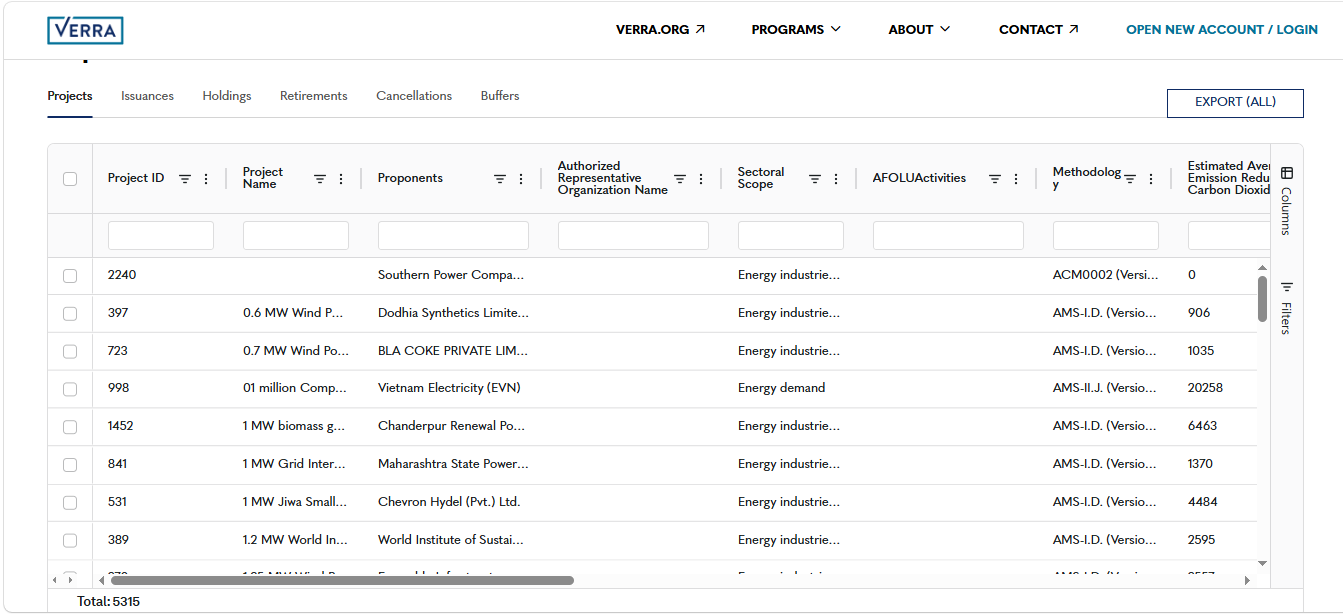
\includegraphics[width=0.85\textwidth]{image/verra_registry.png}
    \caption[Danh sách dự án thuộc chương trình VCS trên Verra Registry]%
    {Danh sách dự án thuộc chương trình VCS trên Verra Registry~\cite{verraregistry}}
    \label{fig:verra}
\end{figure}

National Carbon Credit Registry của UNDP là một hệ thống đăng ký quốc gia mã nguồn mở, xây dựng để các nước triển khai Điều~6~\cite{undp2024nationalregistry}. Hệ thống ghi dữ liệu gốc trong hai sổ cái là sổ cái dự án và sổ cái khối tín chỉ, còn PostgreSQL\index{PostgreSQL} chỉ là cơ sở dữ liệu thứ cấp phục vụ truy vấn. Toàn bộ hệ thống chạy trên AWS theo kiến trúc serverless\index{Serverless}: hàm Lambda \texttt{national-api} xử lý yêu cầu HTTP, còn hàm \texttt{replicator} nhận bản ghi từ luồng Kinesis và sao chép chúng từ sổ cái sang PostgreSQL~\cite{undp2024nationalregistry}. Khi chủ sở hữu chuyển nhượng hoặc hủy một phần của khối tín chỉ (credit block), hệ thống tách dãy số sê-ri thành hai khối để vẫn truy vết được từng tín chỉ; ngoài ra, hệ thống xuất được báo cáo theo Định dạng điện tử thỏa thuận (AEF) của Điều~6.2~\cite{undp2024nationalregistry}.

CAD Trust không cấp tín chỉ mà đóng vai trò một lớp metadata dùng chung, liên kết và chuẩn hóa dữ liệu từ nhiều hệ thống đăng ký như Verra và Gold Standard~\cite{cadtrust2025datamodel}. Mỗi hệ thống đăng ký thành viên chạy một nút của blockchain Chia và tự quản lý dữ liệu của mình; dữ liệu nằm trong cơ sở dữ liệu MySQL, còn mã băm của mỗi lần cập nhật nằm trên blockchain để các bên tự đối chiếu và phát hiện dữ liệu bị sửa~\cite{cadtrust2025datamodel}. Ngày 23/10/2025, CAD Trust công bố mô hình dữ liệu phiên bản 2.0, bổ sung các bảng Stakeholders, Methodologies, Validations, Verifications và các bảng AEF cho Điều~6.2 (Bảng~\ref{tab:cadtrust}). Đồ án dùng mô hình CAD Trust V2.0 làm khung cho cơ sở dữ liệu off-chain.

\begin{table}[!htbp]
    \centering
    \caption{Các thực thể dữ liệu chính trong mô hình CAD Trust V2.0}
    \label{tab:cadtrust}
    \small
    \begin{tabularx}{\textwidth}{|L{3.4cm}|Y|}
        \hline
        \HD{Thực thể (bảng)} & \HD{Thuộc tính khóa và mô tả} \\
        \hline
        Project & Mã dự án trên hệ thống đăng ký gốc, chương trình, lĩnh vực, trạng thái; liên kết với Location và Rating \\
        \hline
        Stakeholders & Bảng mới của V2.0: các tổ chức tham gia dự án và vai trò \\
        \hline
        Validations, Verifications & Bảng mới của V2.0: các đợt validation và verification của dự án \\
        \hline
        Issuances & Mỗi bản ghi là một đợt cấp tín chỉ của dự án \\
        \hline
        Units & Khối tín chỉ với dãy số sê-ri, năm vintage, trạng thái (Issued, Held, Retired); tín chỉ đã hủy có thêm ngày hủy và người thụ hưởng \\
        \hline
        \multicolumn{2}{|l|}{\footnotesize Nguồn: CAD Trust Data Model Version 2.0~\cite{cadtrust2025datamodel}} \\
        \hline
    \end{tabularx}
\end{table}

Toucan Protocol đi theo hướng khác: thay vì xây một hệ thống đăng ký mới, Toucan đưa tín chỉ đã cấp lên các blockchain tương thích Ethereum như Polygon và Celo~\cite{toucan2025docs}. Người dùng tạo một Batch NFT theo chuẩn ERC-721 cho lô tín chỉ của cùng một dự án và cùng năm vintage, sau đó Toucan chia lô đã duyệt thành token TCO2 theo chuẩn ERC-20, mỗi token tương ứng 1~tCO$_2$e. Người giữ TCO2 có thể nạp token vào một pool nếu token đáp ứng tiêu chí của pool đó để đổi lấy token có thể thay thế như Base Carbon Tonne (BCT), hoặc gọi hàm \texttt{retire()} để hủy tín chỉ và nhận một NFT chứng nhận hủy ghi tên bên hủy và người thụ hưởng~\cite{toucan2025docs}. Hiện nay cầu nối từ Verra sang Toucan đã ngừng hoạt động vì Verra không còn chấp nhận cách token hóa này~\cite{toucan2025docs,verra2022crypto}.

Về phía nghiên cứu, Vaccargiu và cộng sự đề xuất một kiến trúc bốn lớp để chứng nhận tín chỉ cho một hệ thống điện mặt trời công suất 100~kWp~\cite{vaccargiu2026blockchain}. Trong kiến trúc này, đồng hồ đo thông minh thu dữ liệu mỗi 1 đến 2 giây, lớp tổng hợp tại biên gom dữ liệu thành các lô 5 phút (288 lần ghi mỗi ngày), và smart contract trên Hyperledger Fabric kiểm tra sản lượng rồi tạo tín chỉ. Nhóm tác giả vẫn giữ bước thẩm định của bên thứ ba, coi blockchain là công cụ hỗ trợ chứ không thay thế quá trình chứng nhận, và chưa mô tả cụ thể cơ chế khóa hay hủy tín chỉ trong smart contract~\cite{vaccargiu2026blockchain}. Liu và cộng sự dùng blockchain dạng đồ thị có hướng không chu trình (DAG) cho giao dịch chứng chỉ năng lượng tái tạo, và theo mô phỏng của nhóm, cách làm này giảm 41\% thời gian giao dịch và 65\% năng lượng tiêu thụ so với cơ chế Proof-of-Stake~\cite{liu2024blockchain}. Hai nghiên cứu này tập trung vào khâu tạo dữ liệu và hiệu năng của sổ cái, trong khi đồ án tập trung vào khâu sau khi tín chỉ đã được cấp, gồm phát hành có kiểm soát, giao dịch và hủy.
% Bản đầy đủ của phần nghiên cứu liên quan (Vaccargiu, Liu, Toucan, Tsai) nằm ở
% backup/2026-11-07_truoc-mau-soict/Chap2.tex, mục sec:lienquan. Không trích Tsai (bản preprint arXiv).

\FloatBarrier
\subsection*{Kết quả quan sát các hệ thống thực tế}
\label{subsec:ks-quansat}

Để kiểm tra các nhận định rút ra từ văn bản, tác giả truy cập trang công khai của các thủ tục và hệ thống liên quan vào ngày 04/11/2026. Bảng~\ref{tab:ks-quansat} tóm tắt kết quả ghi nhận, còn \autoref{fig:ks-dvc-taikhoan} đến \autoref{fig:ks-toucan} là ảnh chụp màn hình các trang này.

\begin{table}[!htbp]
    \centering
    \caption{Kết quả quan sát các hệ thống thực tế}
    \label{tab:ks-quansat}
    \label{tab:ks-quansat-qt}
    \small
    \begin{tabularx}{\textwidth}{|L{3.0cm}|Y|}
        \hline
        \HD{Hệ thống} & \HD{Kết quả ghi nhận} \\
        \hline
        Thủ tục đăng ký tài khoản (mã 1.014129) & Hồ sơ nộp trực tiếp, trực tuyến hoặc qua bưu chính; thời hạn 05 ngày làm việc; hồ sơ qua chuyên viên, lãnh đạo phòng, lãnh đạo Cục và lãnh đạo Bộ duyệt~\cite{mae2026tthc1014129,mae2025qd2935} \\
        \hline
        Thủ tục cấp tín chỉ trong nước (mã 1.014133) & Trang thủ tục vẫn hiển thị quy trình cũ: bộ quản lý lĩnh vực quyết định, tổng 06 ngày làm việc và 30 ngày, có nhánh bổ sung hồ sơ~\cite{mae2026tthc1014133}; từ ngày 12/12/2026, Chủ tịch Ủy ban nhân dân cấp tỉnh quyết định trong tối đa 26 ngày làm việc~\cite{vietnam2026nghidinh396} \\
        \hline
        Sàn giao dịch các-bon (HNX) & VN2025 là mã duy nhất (511.473.846 tấn CO$_2$e hạn ngạch, giao dịch từ 29/6/2026 đến 24/12/2027); khối lượng giao dịch theo tháng rất nhỏ, chưa có tín chỉ nào được giao dịch; trang thống kê giao dịch chưa công bố số liệu tổng hợp (\autoref{fig:ks-hnx}, \autoref{fig:ks-hnx-chitiet}) \\
        \hline
        Verra Registry & Ai cũng tra cứu được, nhưng phát hành, chuyển nhượng, hủy cần tài khoản; báo cáo Retirements công khai từng lô với ngày hủy, dự án, vintage, số sê-ri; người thụ hưởng và lý do hủy có thể ẩn~\cite{verraregistry,verra2020registryv2} \\
        % [VIẾT SAU - SỐ LIỆU] Lọc Retirement Date = 04/11/2026, ghi tổng số lô được hủy trong ngày.
        \hline
        CAD Trust & Dashboard công khai chỉ có số liệu tổng hợp theo khu vực, quốc gia; không tìm thấy trang chi tiết dự án khi không đăng nhập~\cite{cadtrust2026dashboard} \\
        % [VIẾT SAU - ẢNH CHỤP] Chọn Southeast Asia -> Viet Nam trên dashboard, ghi số dự án và nội dung ô Registry.
        \hline
        Toucan Protocol & Trang dự án Wakefield Biochar Facility 2 giữ mã dự án PUR-244045 của tiêu chuẩn gốc Puro và cho biết tín chỉ đã nằm trong pool CHAR~\cite{toucan2026wakefield} \\
        \hline
    \end{tabularx}
\end{table}

\begin{figure}[!htbp]
    \centering
    \begin{subfigure}{\textwidth}
        \centering
        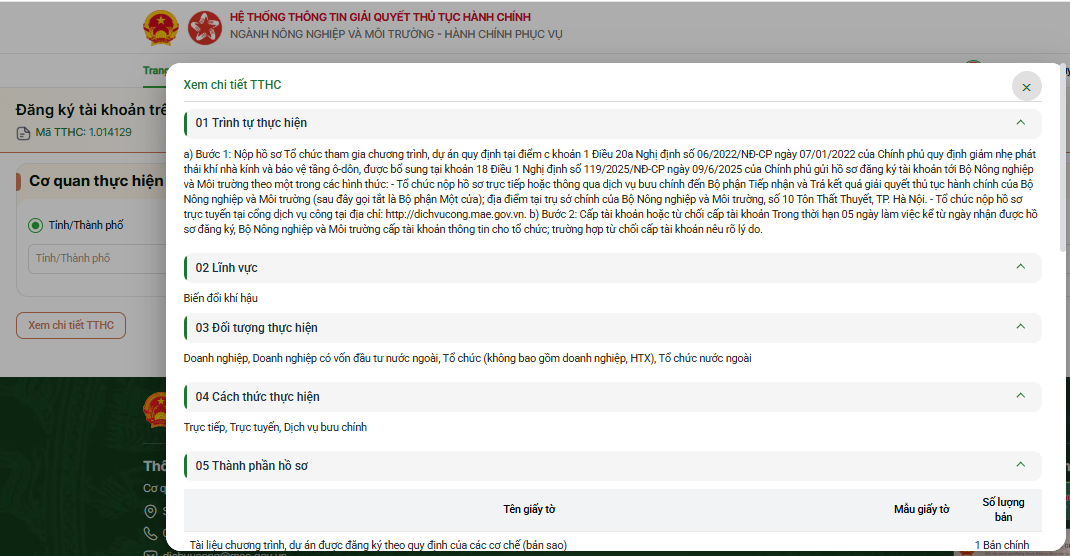
\includegraphics[width=0.8\textwidth]{image/dvc_1014129_trinh_tu.png}
        \caption{Trình tự thực hiện}
    \end{subfigure}

    \vspace{0.3cm}
    \begin{subfigure}{\textwidth}
        \centering
        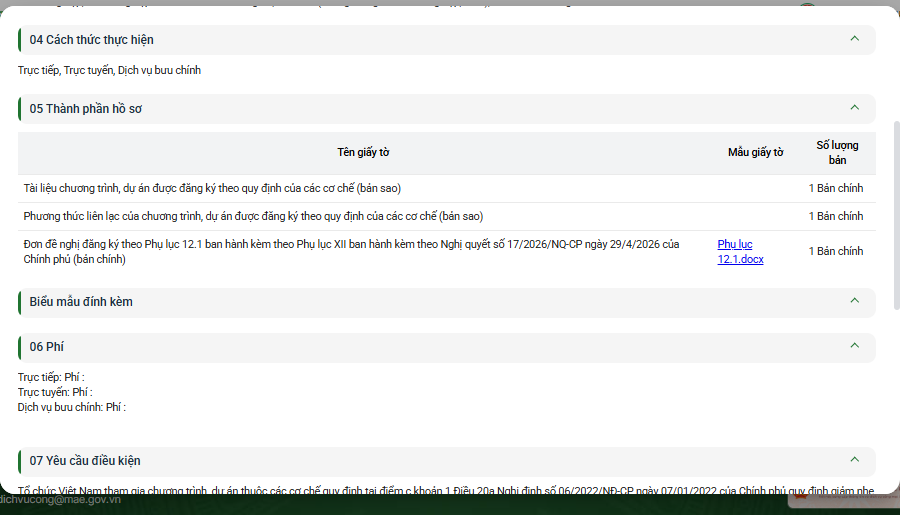
\includegraphics[width=0.68\textwidth]{image/dvc_1014129_ho_so.png}
        \caption{Thành phần hồ sơ}
    \end{subfigure}

    \vspace{0.3cm}
    \begin{subfigure}{\textwidth}
        \centering
        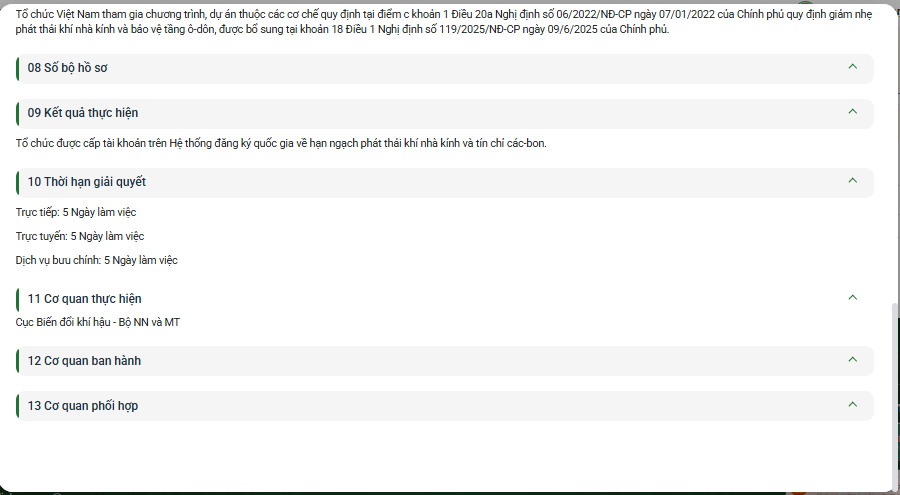
\includegraphics[width=0.68\textwidth]{image/dvc_1014129_thoi_han.png}
        \caption{Kết quả, thời hạn giải quyết và cơ quan thực hiện}
    \end{subfigure}
    \caption[Trang thủ tục đăng ký tài khoản trên Hệ thống đăng ký quốc gia]%
    {Trang thủ tục mã 1.014129 về đăng ký tài khoản trên Hệ thống đăng ký quốc gia (truy cập ngày 04/11/2026)~\cite{mae2026tthc1014129}}
    \label{fig:ks-dvc-taikhoan}
\end{figure}

\begin{figure}[!htbp]
    \centering
    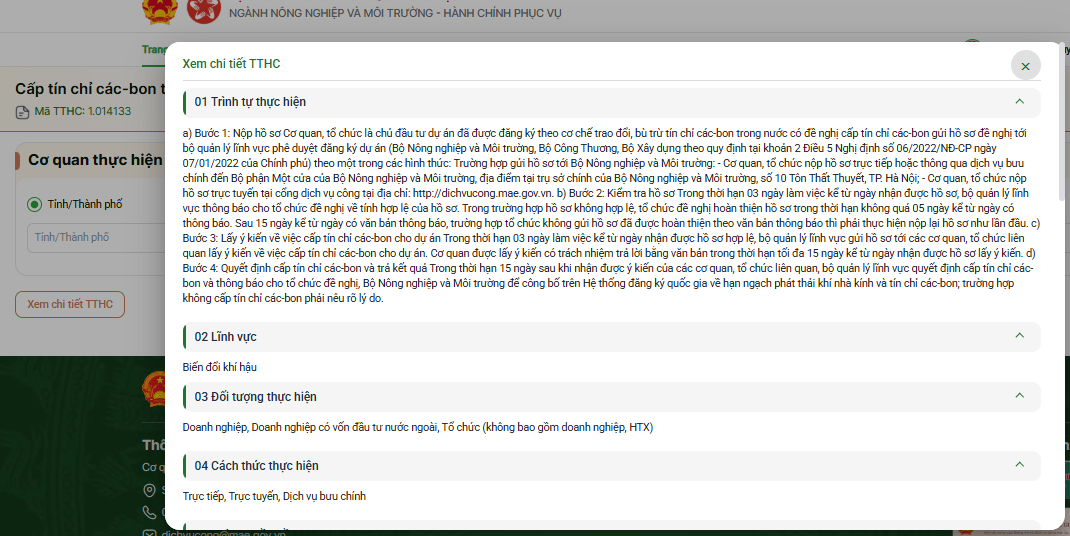
\includegraphics[width=0.85\textwidth]{image/dvc_1014133_trinh_tu.png}
    \caption[Trang thủ tục cấp tín chỉ các-bon theo cơ chế trong nước]%
    {Trang thủ tục mã 1.014133 về cấp tín chỉ các-bon theo cơ chế trong nước, trình tự bốn bước trước Nghị định 396/2026/NĐ-CP (truy cập ngày 04/11/2026)~\cite{mae2026tthc1014133}}
    \label{fig:ks-dvc-tinchi}
\end{figure}

\begin{figure}[!htbp]
    \centering
    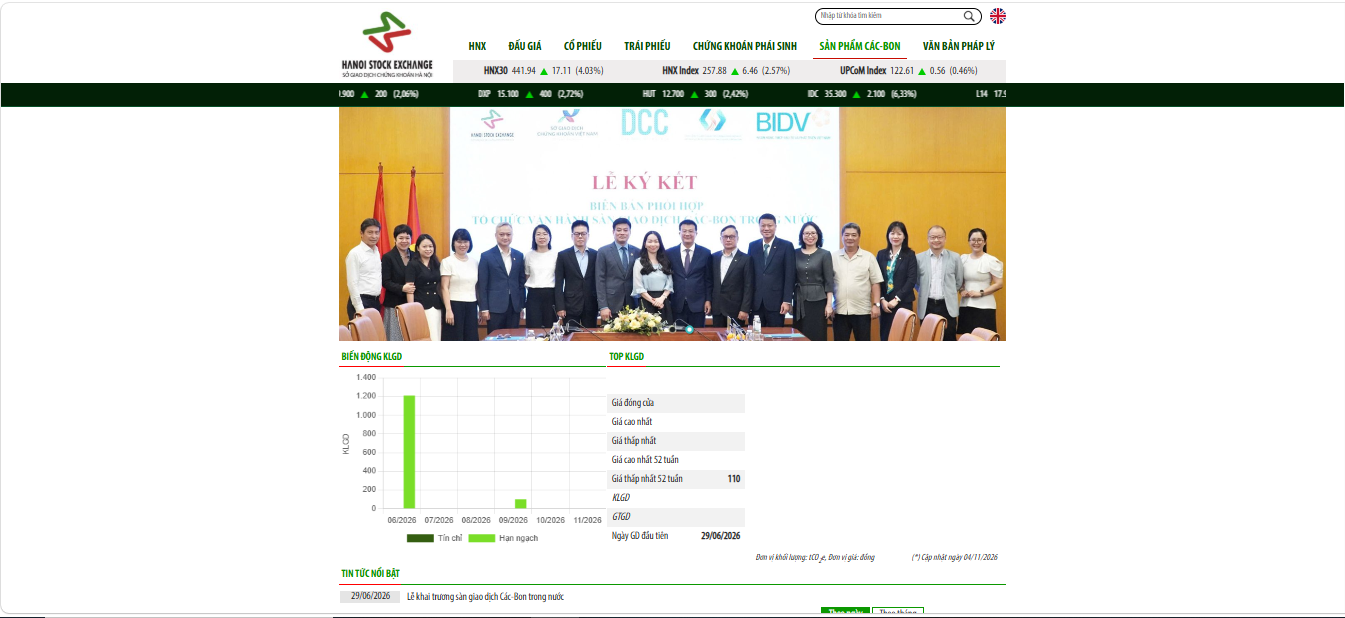
\includegraphics[width=0.9\textwidth]{image/hnx_san_cacbon.png}
    \caption[Trang sản phẩm các-bon trên website của HNX]%
    {Trang sản phẩm các-bon của HNX: khối lượng giao dịch theo tháng và thông tin mã VN2025 (truy cập ngày 04/11/2026)}
    \label{fig:ks-hnx}
\end{figure}

\begin{figure}[!htbp]
    \centering
    \begin{subfigure}{\textwidth}
        \centering
        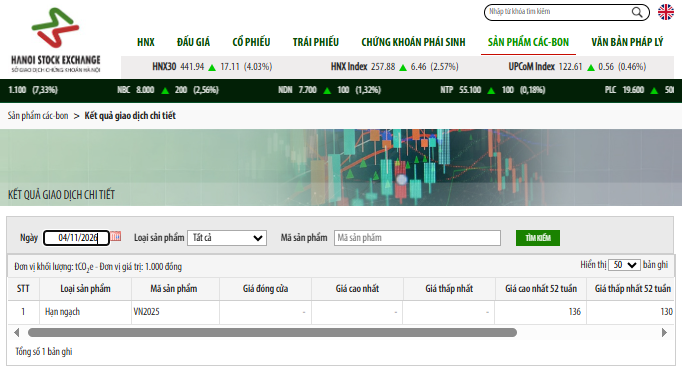
\includegraphics[width=0.75\textwidth]{image/hnx_ket_qua_giao_dich.png}
        \caption{Kết quả giao dịch chi tiết ngày 04/11/2026}
    \end{subfigure}

    \vspace{0.3cm}
    \begin{subfigure}{\textwidth}
        \centering
        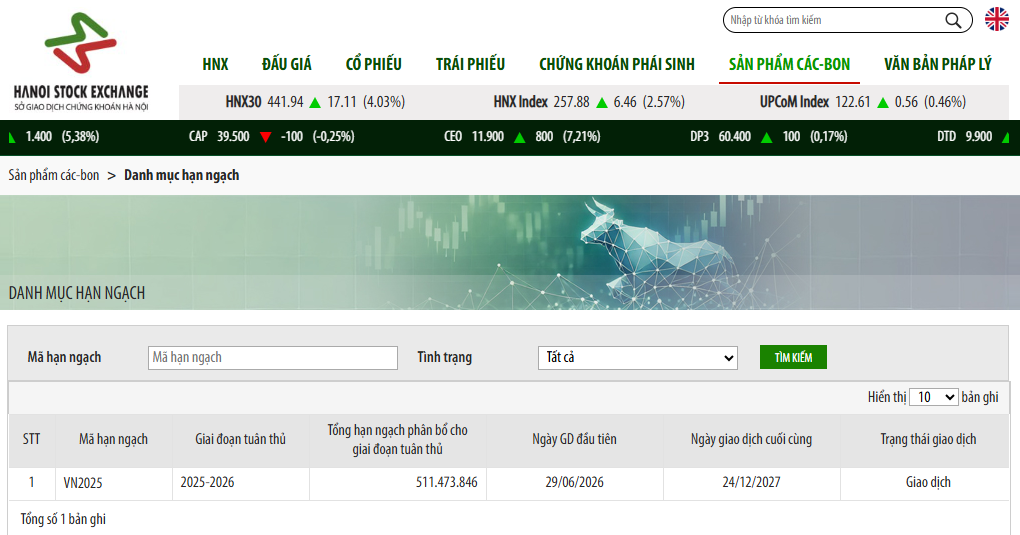
\includegraphics[width=0.85\textwidth]{image/hnx_danh_muc_han_ngach.png}
        \caption{Danh mục hạn ngạch}
    \end{subfigure}
    \caption[Kết quả giao dịch và danh mục hạn ngạch trên website của HNX]%
    {Kết quả giao dịch và danh mục hạn ngạch trên trang sản phẩm các-bon của HNX (truy cập ngày 04/11/2026)}
    \label{fig:ks-hnx-chitiet}
\end{figure}

\begin{figure}[!htbp]
    \centering
    \begin{subfigure}{\textwidth}
        \centering
        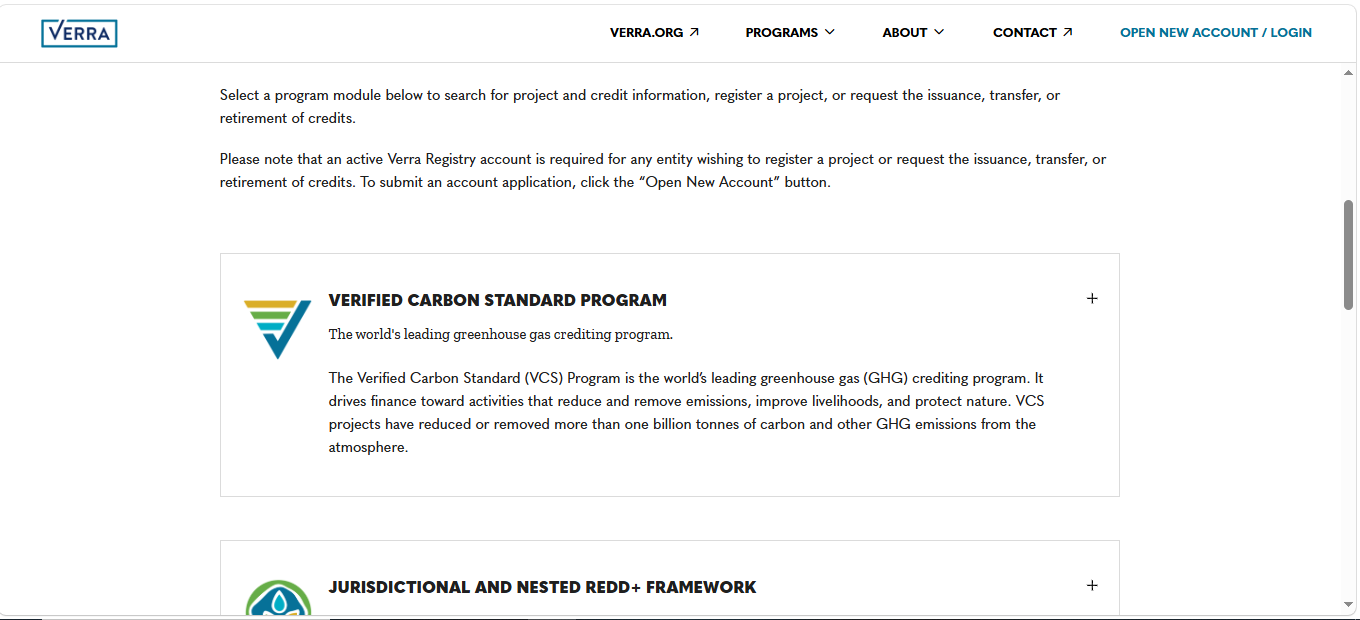
\includegraphics[width=0.85\textwidth]{image/verra_registry_home.png}
        \caption{Trang chủ: tra cứu theo chương trình là công khai, còn đăng ký, phát hành, chuyển nhượng và hủy tín chỉ yêu cầu tài khoản~\cite{verraregistry}}
    \end{subfigure}

    \vspace{0.3cm}
    \begin{subfigure}{\textwidth}
        \centering
        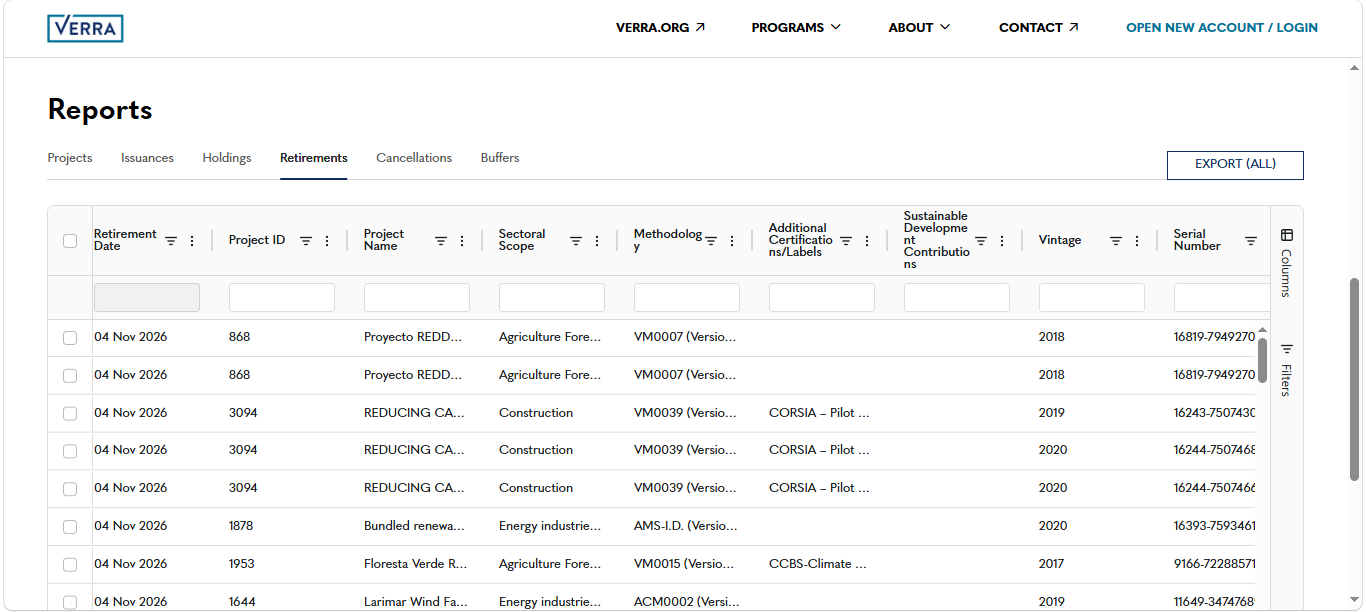
\includegraphics[width=0.85\textwidth]{image/verra_retirements.png}
        \caption{Báo cáo Retirements: mỗi dòng là một lô tín chỉ đã hủy, có ngày hủy, dự án, vintage và số sê-ri~\cite{verraregistry}}
    \end{subfigure}
    \caption[Trang công khai của Verra Registry]%
    {Trang công khai của Verra Registry (truy cập ngày 04/11/2026)}
    \label{fig:ks-verra}
\end{figure}

% [VIẾT SAU - ẢNH CHỤP] Thay bằng ảnh dashboard của Việt Nam (Southeast Asia -> Viet Nam) và sửa chú thích.
\begin{figure}[!htbp]
    \centering
    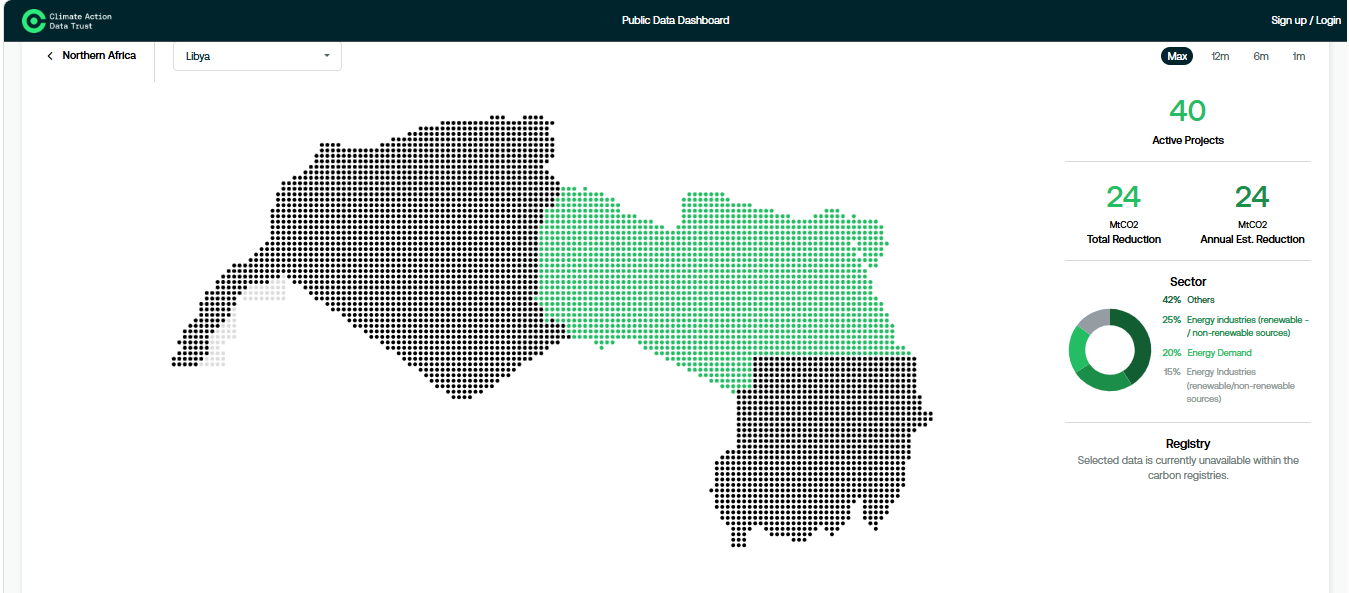
\includegraphics[width=0.85\textwidth]{image/cadtrust_dashboard.png}
    \caption[Public Data Dashboard của CAD Trust]%
    {Public Data Dashboard của CAD Trust: số liệu tổng hợp của một quốc gia gồm số dự án, lượng giảm phát thải và cơ cấu theo lĩnh vực (truy cập ngày 04/11/2026)~\cite{cadtrust2026dashboard}}
    \label{fig:ks-cadtrust}
\end{figure}

\begin{figure}[!htbp]
    \centering
    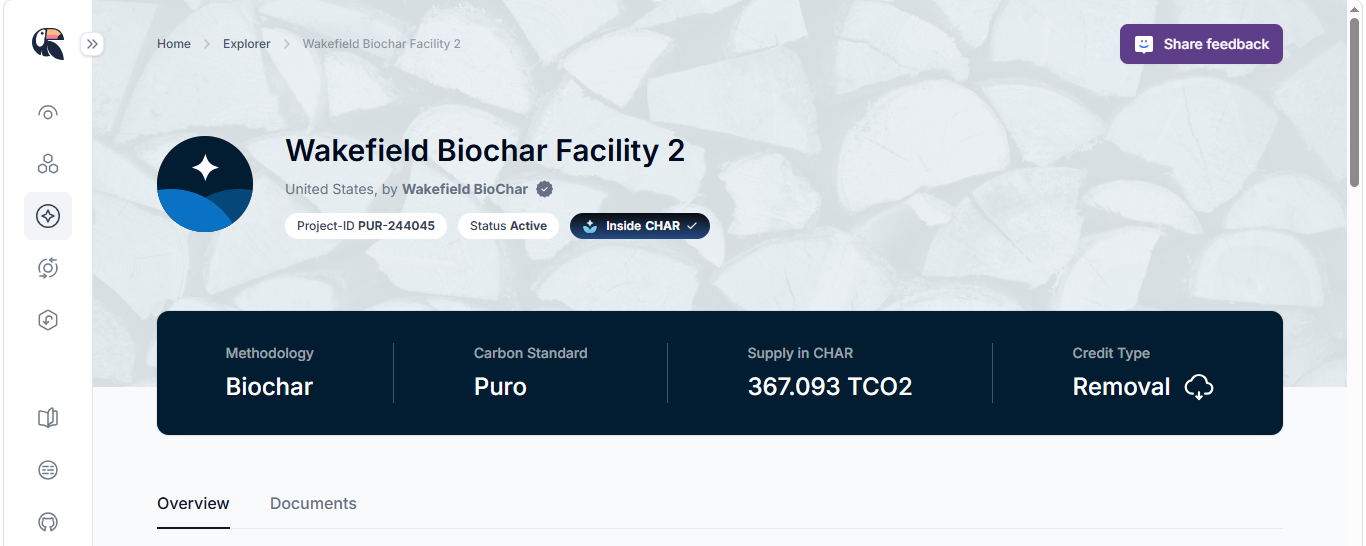
\includegraphics[width=0.85\textwidth]{image/toucan_project.png}
    \caption[Trang một dự án trên ứng dụng Toucan]%
    {Trang dự án Wakefield Biochar Facility 2 trên ứng dụng Toucan: mã dự án, tiêu chuẩn gốc, phương pháp luận, loại tín chỉ và pool chứa token (truy cập ngày 04/11/2026)~\cite{toucan2026wakefield}}
    \label{fig:ks-toucan}
\end{figure}

Kết quả quan sát cho thấy hai đặc điểm của hệ thống trong nước. Đặc điểm thứ nhất là nghiệp vụ đi qua nhiều cấp phê duyệt và nhiều hệ thống: một giao dịch cần dữ liệu ở Hệ thống đăng ký quốc gia, hệ thống giao dịch của HNX, hệ thống lưu ký của VSDC và tài khoản tại công ty chứng khoán, còn mỗi bước của thủ tục cấp tín chỉ có thời hạn riêng và có nhánh quay lại khi hồ sơ cần bổ sung. Theo Nghị định 396/2026/NĐ-CP, từ ngày 12/12/2026 việc cấp tín chỉ trong nước mất tối đa 26 ngày làm việc, so với khoảng 27 đến 28 ngày làm việc của quy trình cũ~\cite{vietnam2026nghidinh396}. Thay đổi đáng chú ý hơn là thẩm quyền chuyển xuống cấp tỉnh: nhiều địa phương sẽ cùng cấp tín chỉ nhưng vẫn phải ghi nhận thống nhất trên Hệ thống đăng ký quốc gia, nên hệ thống mới cần cho phép nhiều tài khoản cùng có quyền phát hành (NC-09). Đặc điểm thứ hai là thị trường chưa có thanh khoản: đến ngày 04/11/2026, hàng hóa duy nhất trên sàn là hạn ngạch, nên hiện chưa có dữ liệu thực tế về giao dịch tín chỉ trong nước để đưa vào hệ thống.

Với các hệ thống quốc tế, Verra Registry tách rõ phần tra cứu công khai và phần nghiệp vụ cần tài khoản. Báo cáo hủy tín chỉ của Verra công khai tới từng lô và số sê-ri nhưng cho phép ẩn người thụ hưởng, nghĩa là yêu cầu minh bạch luôn đi kèm giới hạn về quyền riêng tư. Các hệ thống tổng hợp dữ liệu hoặc token hóa tín chỉ đều dựa vào hệ thống đăng ký gốc: CAD Trust chỉ hiển thị được số liệu mà các hệ thống đăng ký cung cấp, còn dự án Wakefield Biochar Facility 2 trên Toucan là tín chỉ do Puro cấp và vẫn giữ mã dự án của Puro. Điều này dẫn tới yêu cầu mỗi bản ghi tín chỉ trên blockchain phải giữ liên kết tới mã dự án và số sê-ri do hệ thống đăng ký gốc cấp.

\FloatBarrier
\subsection*{Đánh giá hiện trạng}
\label{subsec:ks-danhgia}

Hệ thống trong nước có cơ sở pháp lý rõ ràng, dữ liệu gốc thống nhất, số sê-ri tới từng tấn CO$_2$e, mô hình tám tiểu khoản chặt chẽ và định danh pháp lý qua Cổng dịch vụ công quốc gia. Các hệ thống quốc tế đóng góp những ý tưởng mà hệ thống mới có thể kế thừa, gồm tra cứu công khai của Verra, mã nguồn mở và cách tách khối sê-ri của UNDP, mô hình dữ liệu chung của CAD Trust và việc hủy tín chỉ công khai trên blockchain của Toucan. Bảng~\ref{tab:ks-uunhuoc} so sánh ưu, nhược điểm của từng hệ thống.

\begin{table}[!htbp]
    \centering
    \caption{Ưu điểm và nhược điểm của các hệ thống được khảo sát}
    \label{tab:ks-uunhuoc}
    \small
    \begin{tabularx}{\textwidth}{|L{2.8cm}|Y|Y|}
        \hline
        \HD{Hệ thống} & \HD{Ưu điểm} & \HD{Nhược điểm} \\
        \hline
        Hệ thống trong nước & Pháp lý rõ ràng; dữ liệu gốc thống nhất; số sê-ri tới từng đơn vị; xác thực định danh điện tử & Đang thí điểm; ba hệ thống phải đối soát cuối ngày; công khai chủ yếu ở dạng tổng hợp; bên ngoài không tự kiểm tra được lịch sử tín chỉ \\
        \hline
        Verra Registry & Quy mô lớn; số sê-ri duy nhất; tra cứu công khai & Tập trung; chưa có API công khai; không liên thông với hệ thống khác \\
        \hline
        UNDP National Carbon Registry & Mã nguồn mở; hỗ trợ Điều~6 và AEF; tách dãy sê-ri & Mỗi quốc gia tự vận hành hạ tầng; sổ cái do một bên quản lý \\
        \hline
        CAD Trust & Liên thông nhiều hệ thống; mô hình dữ liệu chung; mã băm trên blockchain & Không ghi quyền sở hữu, không giao dịch; mã băm chứng minh dữ liệu không bị sửa, không chứng minh dữ liệu đúng \\
        \hline
        Toucan Protocol & Hủy tín chỉ và chứng nhận hủy công khai on-chain & Phụ thuộc hệ thống đăng ký gốc; Verra đã cấm token hóa tín chỉ đã hủy~\cite{verra2022crypto}; pool làm mất thông tin riêng của dự án \\
        \hline
    \end{tabularx}
\end{table}

Hệ thống trong nước có năm nhược điểm chính. Nhược điểm lớn nhất là tính toàn vẹn dựa vào niềm tin vào đơn vị vận hành: phần mềm và quy trình của cơ quan quản lý bảo đảm các ràng buộc như không cấp lại mã trong nước đã hủy hay không hủy quá số dư, nhưng bên mua hoặc tổ chức bên ngoài không có công cụ để tự kiểm tra rằng một số sê-ri chưa từng được cấp cho người khác hoặc chưa từng bị hủy. Nhược điểm thứ hai là dữ liệu phân tán: Hệ thống đăng ký quốc gia và hệ thống lưu ký của VSDC cùng ghi một lượng tín chỉ, nên hai bên phải đối soát cuối mỗi ngày và duy trì quy trình xử lý sai lệch~\cite{vietnam2026thongtu11}. Nhược điểm thứ ba là độ trễ trong nghiệp vụ, vì đề nghị ký gửi phải chờ tổng hợp cuối ngày và chờ VSDC xác nhận trong 01 ngày làm việc, còn yêu cầu hủy tự nguyện mất 02 ngày làm việc~\cite{vietnam2026thongtu11}.

Hai nhược điểm còn lại liên quan đến dữ liệu công khai và hồ sơ. Dữ liệu mà Bộ công bố chủ yếu là số liệu tổng hợp theo tháng, năm, còn thông tin giao dịch thuộc diện bảo mật; cách làm này đáp ứng yêu cầu bảo mật nhưng khiến bên thứ ba khó truy vết lịch sử của một tín chỉ cụ thể, và tại thời điểm khảo sát hệ thống chưa có tài liệu API công khai cho bên thứ ba. Ngoài ra, khâu MRV chưa được số hóa đồng bộ: hồ sơ dự án, báo cáo giám sát và báo cáo thẩm định vẫn là các tệp nộp qua từng bước, chưa gắn với tín chỉ đã cấp bằng một dấu vết kiểm tra (audit trail) mà bên ngoài xác minh được~\cite{mae2026tthc1014133}.

Các nhược điểm trên quy về năm vấn đề làm cơ sở cho nhu cầu của hệ thống mới. Mỗi vấn đề có một mã riêng để Bảng~\ref{tab:ks-nhucauchucnang} tham chiếu lại.
\begin{enumerate}[label=VĐ-\arabic*., leftmargin=1.6cm]
    \item Rủi ro phát hành kép giữa các hệ thống: hệ thống trong nước và các chương trình quốc tế dùng các hệ mã định danh khác nhau, nên nếu không liên thông dữ liệu thì một dự án có thể đăng ký ở nhiều nơi~\cite{schneider2019double}.
    \item Bên mua khó chứng minh tín chỉ đã bị hủy: bằng chứng hiện nay chủ yếu là thông báo xác nhận mà cơ quan quản lý gửi cho chủ tài khoản, và bên thứ ba không tự kiểm tra được thông báo này.
    \item Hồ sơ MRV và thẩm định không gắn chặt với tín chỉ: chưa có cơ chế kỹ thuật nào bảo đảm hồ sơ không bị sửa sau khi cấp hoặc không bị dùng lại cho một lần cấp khác.
    \item Chi phí đối soát giữa nhiều cơ sở dữ liệu: ba hệ thống cùng ghi một lượng tín chỉ, nên các bên phải đối soát cuối mỗi ngày và duy trì quy trình xử lý sai lệch~\cite{vietnam2026thongtu11}.
    \item Thị trường còn ở giai đoạn đầu và quy định thay đổi nhanh, ví dụ việc phân cấp cho cấp tỉnh theo Nghị định 396/2026/NĐ-CP~\cite{vietnam2026nghidinh396}, nên hệ thống mới cần linh hoạt trong phân quyền.
\end{enumerate}

\FloatBarrier
\subsection*{Các tính năng cần phát triển}
\label{subsec:ks-nhucau}

Hệ thống mới không thay thế Hệ thống đăng ký quốc gia mà là một nguyên mẫu bổ sung, dùng để thử nghiệm việc biến các ràng buộc nghiệp vụ đã có trong quy định (số sê-ri duy nhất, không hủy hai lần, không chuyển nhượng tín chỉ đã hủy) thành ràng buộc kỹ thuật mà ai cũng kiểm tra được. Năm vấn đề VĐ-1 đến VĐ-5 ở phần đánh giá hiện trạng dẫn tới mười nhu cầu chức năng (Bảng~\ref{tab:ks-nhucauchucnang}). Trong cột Vấn đề, ``một phần'' nghĩa là nhu cầu chỉ giải quyết vấn đề bên trong hệ thống, còn dấu ``--'' nghĩa là nhu cầu phục vụ vận hành. Các nhu cầu này là đầu vào cho biểu đồ use case và đặc tả chức năng của hệ thống.

\begin{table}[!htbp]
    \centering
    \caption{Nhu cầu chức năng của hệ thống mới}
    \label{tab:ks-nhucauchucnang}
    \small
    \begin{tabularx}{\textwidth}{|L{1.3cm}|Y|L{2.8cm}|L{2.1cm}|}
        \hline
        \HD{Mã} & \HD{Nhu cầu} & \HD{Bên liên quan} & \HD{Vấn đề} \\
        \hline
        NC-01 & Đăng ký dự án, tải lên hồ sơ (PDD, báo cáo giám sát), lưu mã băm hồ sơ & Chủ dự án & VĐ-3 \\
        \hline
        NC-02 & Gửi yêu cầu cấp tín chỉ; VVB phê duyệt hoặc từ chối & Chủ dự án, VVB & VĐ-3 \\
        \hline
        NC-03 & Phát hành lô tín chỉ có dãy sê-ri duy nhất; từ chối dãy sê-ri trùng hoặc hồ sơ đã dùng & Cơ quan quản lý & VĐ-1 (một phần), VĐ-3 \\
        \hline
        NC-04 & Chuyển nhượng tín chỉ giữa các ví, ghi lịch sử sở hữu công khai & Chủ dự án, doanh nghiệp & VĐ-2, VĐ-4 \\
        \hline
        NC-05 & Giao dịch từng phần của một lô qua pool token có thể thay thế & Chủ dự án, doanh nghiệp & -- \\
        \hline
        NC-06 & Hủy tín chỉ từ lô hoặc từ pool, ghi người thụ hưởng và dãy sê-ri bị hủy; tín chỉ đã hủy không chuyển nhượng hay hủy lại được & Doanh nghiệp & VĐ-2 \\
        \hline
        NC-07 & Tra cứu công khai theo số sê-ri, xem chứng nhận hủy kèm liên kết giao dịch on-chain & Người dùng công khai & VĐ-2 \\
        \hline
        NC-08 & Dashboard so sánh tín chỉ đã hủy với lượng phát thải hoặc hạn ngạch khai báo & Doanh nghiệp & VĐ-2 \\
        \hline
        NC-09 & Quản lý vai trò VVB và phát hành; nhiều tài khoản cùng có quyền phát hành (mỗi tỉnh một tài khoản), ghi tài khoản đã phát hành từng lô; tạm dừng khi có sự cố & Cơ quan quản lý & VĐ-5 \\
        \hline
        NC-10 & Xuất dữ liệu dự án, đợt cấp, đơn vị tín chỉ theo cấu trúc CAD Trust V2.0 & Cơ quan quản lý, hệ thống ngoài & VĐ-1 (một phần) \\
        \hline
    \end{tabularx}
\end{table}

% ------------------------------------------------------------
% [VIẾT SAU] Mục Tổng quan chức năng (mẫu SoICT 2.2) — bỏ dấu % để khôi phục khi viết.
% Đã thống nhất (07/11/2026): VVB thẩm định, phê duyệt; cơ quan quản lý phát hành (mint). Hình \HinhUseCase
% (figures_chap3.tex) đã sửa theo cách này. Mã nguồn contracts/CarbonCreditNFT.sol vẫn để mintBatch cho
% VERIFIER_ROLE, cần thêm vai trò phát hành (ISSUER_ROLE) cho cơ quan quản lý.
% \section{Tổng quan chức năng}
% \label{sec:tongquanchucnang}
% % Chỉ mô tả chức năng mức cao; đặc tả chi tiết ở mục Đặc tả chức năng.
%
% \subsection*{Biểu đồ use case tổng quát}
% \label{subsec:usecase}
% % Vẽ biểu đồ use case tổng quát, giải thích các tác nhân (Chủ dự án, VVB, Cơ quan quản lý,
% % Doanh nghiệp mua, Người xem công khai), vai trò của từng tác nhân và các use case chính.
% % Mỗi use case nên ghi mã NC tương ứng ở Bảng tab:ks-nhucauchucnang.
% % [VIẾT SAU] \canviet{Biểu đồ use case tổng quát}
%
% \subsection*{Biểu đồ use case phân rã ``Phát hành tín chỉ''}
% % Tên mục phải khớp tên use case trong biểu đồ tổng quát. Mỗi use case mức cao một mục riêng,
% % ví dụ thêm ``Giao dịch tín chỉ'', ``Hủy tín chỉ''.
% % [VIẾT SAU] \canviet{Biểu đồ use case phân rã}
%
% \subsection*{Quy trình nghiệp vụ}
% % Biểu đồ hoạt động cho quy trình kết hợp nhiều use case: đăng ký dự án -> gửi yêu cầu cấp ->
% % VVB phê duyệt -> cơ quan quản lý phát hành -> nạp pool -> bán từng phần -> doanh nghiệp hủy.
% % [VIẾT SAU] \canviet{Quy trình nghiệp vụ}
%
% % ------------------------------------------------------------
% \section{Đặc tả chức năng}
% \label{sec:dactachucnang}
% % Chọn 4–7 use case quan trọng nhất. Mỗi đặc tả có ít nhất: tên use case, luồng sự kiện
% % (chính và phát sinh), tiền điều kiện, hậu điều kiện. Chỉ vẽ biểu đồ hoạt động khi use case phức tạp.
% % Gợi ý: Gửi yêu cầu cấp tín chỉ; Phê duyệt kết quả thẩm định; Phát hành lô tín chỉ;
% % Nạp lô vào pool; Hủy tín chỉ từ pool; Tra cứu theo số sê-ri.
% % Mọi use case ghi on-chain đều có tiền điều kiện ``đã kết nối ví MetaMask''.
% \subsection*{Đặc tả use case ``Phát hành lô tín chỉ''}
% % [VIẾT SAU] \canviet{Đặc tả use case}
% \subsection*{Đặc tả use case ``Hủy tín chỉ''}
% % [VIẾT SAU] \canviet{Đặc tả use case}

% ------------------------------------------------------------
\section{Yêu cầu phi chức năng}
\label{sec:phichucnang}
\label{subsec:ycphichucnang}

Ngoài các chức năng ở Bảng~\ref{tab:ks-nhucauchucnang}, hệ thống phải đáp ứng một số yêu cầu phi chức năng, trong đó quan trọng nhất là tính toàn vẹn và khả năng kiểm tra. Mỗi dãy sê-ri chỉ phát hành một lần, quyền sở hữu và trạng thái hủy lấy dữ liệu on-chain làm gốc, và bên thứ ba phải tự kiểm tra được lịch sử của một tín chỉ mà không cần hỏi đơn vị vận hành. Cơ sở dữ liệu off-chain chỉ là bản sao phục vụ truy vấn, nên khi hai phía lệch nhau thì hệ thống lấy dữ liệu on-chain làm chuẩn.

Về bảo mật, chỉ những tài khoản có vai trò phù hợp mới được phát hành tín chỉ hoặc thay đổi vai trò, và smart contract phải chống được các lỗ hổng phổ biến như reentrancy. Yêu cầu này đi cùng yêu cầu về quyền riêng tư, vì Thông tư 11/2026/TT-BNNMT vừa yêu cầu công khai thông tin (Điều~4) vừa yêu cầu bảo mật thông tin giao dịch (Điều~24)~\cite{vietnam2026thongtu11}. Để dung hòa hai yêu cầu đó, hệ thống chỉ ghi on-chain địa chỉ ví, dãy sê-ri, trạng thái và mã băm hồ sơ; thông tin định danh doanh nghiệp, hồ sơ và giá giao dịch nằm off-chain và có phân quyền truy cập, giống cách CAD Trust và Verra đang làm~\cite{cadtrust2025datamodel,verra2020registryv2}.

Về chi phí, hệ thống cần giữ chi phí gas của các thao tác chính ở mức chấp nhận được, và quá trình kiểm thử sẽ đo chi phí này. Về khả năng tương thích và bảo trì, dữ liệu off-chain theo mô hình CAD Trust V2.0, còn kiến trúc tách lớp để sau này bổ sung chữ ký số của VVB, kết nối dữ liệu MRV hay ánh xạ sang mã trong nước mà không phải sửa smart contract đã triển khai. Về tính dễ dùng, giao diện hướng dẫn người dùng từng bước khi kết nối và ký giao dịch bằng ví MetaMask, vì phần lớn người dùng nghiệp vụ chưa quen với ví blockchain.

% ------------------------------------------------------------
% Kết chương (định dạng Normal, không tiêu đề — theo mẫu SoICT).
Qua chương này, tác giả đã xác định vấn đề trung tâm của đề tài là tính toàn vẹn của tín chỉ các-bon, cụ thể là nguy cơ tính toán kép khi dữ liệu nằm ở nhiều hệ thống và bên ngoài không tự kiểm tra được. Kết quả khảo sát cho thấy Việt Nam đã có hạ tầng pháp lý và kỹ thuật tương đối đầy đủ cho thị trường các-bon trong nước; khoảng trống mà đồ án hướng tới không nằm ở việc thiếu một hệ thống quản lý, mà ở chỗ các ràng buộc chống tính toán kép đang dựa vào niềm tin vào đơn vị vận hành và vào việc đối soát giữa nhiều cơ sở dữ liệu. Từ năm vấn đề VĐ-1 đến VĐ-5, tác giả rút ra mười nhu cầu chức năng và các yêu cầu phi chức năng, đồng thời chọn hướng giải quyết là kiến trúc lai, trong đó smart contract trên Ethereum đảm nhận ba thao tác phát hành, chuyển nhượng và hủy tín chỉ. Chương 2 sẽ trình bày các công nghệ mà đồ án dùng để hiện thực hướng giải pháp này và lý do lựa chọn từng công nghệ.
% [VIẾT SAU] Khi khôi phục Chương 2: "Chương~\ref{chap:congnghe}" thay cho "Chương 2".


% Chương 2 = mẫu SoICT chương 3 "Công nghệ sử dụng".
% [VIẾT SAU] Bản nộp hiện tại chỉ tới Chương 1 — bỏ dấu % ở dòng dưới để khôi phục.
% % ============================================================
% CHƯƠNG 2 — CÔNG NGHỆ SỬ DỤNG  (mẫu SoICT chương 3)
% Sắp xếp lại ngày 07/11/2026 theo mẫu Do_An_Latex_SoiCT. Bản trước: backup/2026-11-07_truoc-mau-soict/Chap2.tex
% (tên cũ "CƠ SỞ LÝ THUYẾT VÀ CÔNG NGHỆ"). Mục "Các nghiên cứu và hệ thống liên quan" (sec:lienquan:
% Vaccargiu, Liu, Toucan, Tsai) đã chuyển, rút gọn, vào Chương 1 mục 1.5.4 (subsec:verra-undp) vì mẫu SoICT
% đặt khảo sát hệ thống tương tự ở chương khảo sát; bản đầy đủ vẫn nằm trong file backup.
%
% Hướng dẫn của mẫu SoICT cho chương này:
%   - không quá 10 trang; nội dung dài hơn đưa vào Phụ lục; phân tích và tóm tắt, không trình bày dài dòng;
%   - chỉ giới thiệu công nghệ, nền tảng, thư viện mà đồ án thực sự dùng; không trình bày lại kiến thức
%     phổ thông hay sách giáo khoa;
%   - với mỗi công nghệ: (i) nó giải quyết vấn đề / yêu cầu nào ở Chương 1 (NC-xx, VĐ-x, yêu cầu phi chức năng),
%     (ii) các phương án thay thế, (iii) lý do chọn; có thể dùng bảng so sánh;
%   - phần thiết kế, cài đặt cụ thể để ở Chương 3.
% Văn phong: đoạn văn liên kết, câu chủ động có chủ ngữ thật ("đồ án", "Ethereum", "MetaMask"...; hạn chế xưng
% "em", "tác giả" chỉ dùng ở Kết chương), mục con dùng \subsection*,
% giữ thuật ngữ tiếng Anh (smart contract, token, gas, testnet...). Xem ghi chú đầu Chap1.tex.
% ============================================================

\chapter{CÔNG NGHỆ SỬ DỤNG}
\label{chap:congnghe}
\label{chap:cosolythuyet}
% ============================================================
% HÌNH VẼ CHƯƠNG 2 (TikZ) — gọi bằng macro trong Chap2.tex
%   \HinhChuoiKhoi  : cấu trúc liên kết các khối          (fig:chuoikhoi)
%   \HinhLuongDApp  : luồng tương tác của dApp             (fig:luongdapp)
% ============================================================

% ---------- Cấu trúc liên kết các khối ----------
\newcommand{\HinhChuoiKhoi}{%
\begin{figure}[htbp]
\centering
\begin{tikzpicture}[
    >=Stealth,
    truong/.style={draw, minimum width=3.3cm, minimum height=0.55cm,
                   font=\footnotesize, fill=white, inner sep=1pt},
    tieude/.style={truong, fill=gray!20, font=\footnotesize\bfseries}]
  \foreach \i/\x/\ten in {0/0/N-1, 1/4.6/N, 2/9.2/N+1} {
    \node[tieude] (h\i) at (\x,0) {Khối \ten};
    \node[truong, below=0pt of h\i] (p\i) {Mã băm khối trước};
    \node[truong, below=0pt of p\i] (t\i) {Dấu thời gian};
    \node[truong, below=0pt of t\i] (m\i) {Gốc Merkle};
    \node[truong, below=0pt of m\i, minimum height=1cm, align=center] (g\i)
        {Danh sách\\giao dịch};
    \node[draw, thick, rounded corners=2pt, inner sep=3pt, fit=(h\i)(g\i)] (b\i) {};
  }
  \draw[->, thick] (p1.west) -- (b0.east |- p1.west);
  \draw[->, thick] (p2.west) -- (b1.east |- p2.west);
  \node[font=\large] at (-2.35,-1.4) {$\cdots$};
  \node[font=\large] at (11.55,-1.4) {$\cdots$};
\end{tikzpicture}
\caption[Cấu trúc liên kết giữa các khối trong chuỗi khối]{Cấu trúc liên kết giữa các khối trong chuỗi khối \hinhtao[Claude]{20/10/2026}}
\label{fig:chuoikhoi}
\end{figure}}

% ---------- Luồng tương tác của ứng dụng phi tập trung ----------
\newcommand{\HinhLuongDApp}{%
\begin{figure}[htbp]
\centering
\begin{tikzpicture}[
    >=Stealth,
    hop/.style={draw, rounded corners=3pt, align=center, font=\footnotesize,
                text width=2.1cm, minimum height=1.1cm, fill=white},
    nhan/.style={font=\scriptsize, align=center}]
  \node[hop]                         (u)   at (0,0)     {Người dùng};
  \node[hop]                         (fe)  at (3.7,0)   {Giao diện web\\(Next.js,\\ethers.js)};
  \node[hop]                         (mm)  at (7.4,0)   {Ví\\MetaMask\\(giữ khóa riêng)};
  \node[hop, text width=2.6cm, minimum height=1.6cm, fill=gray!12]
                                     (net) at (11.3,0)  {Mạng Ethereum\\(Sepolia)\\nút RPC, EVM,\\hợp đồng thông minh};
  \node[hop]                         (be)  at (3.7,-3)  {Backend\\(Node.js, Express)};
  \node[hop]                         (db)  at (0,-3)    {CSDL off-chain\\(PostgreSQL)};

  \draw[->] (u) -- node[nhan, above] {thao tác} (fe);
  \draw[->] (fe) -- node[nhan, above] {yêu cầu ký\\(EIP-1193)} (mm);
  \draw[->] (mm) -- node[nhan, above] {giao dịch\\đã ký} (net);
  \draw[->, dashed] (fe.north) to[bend left=22]
      node[nhan, above] {đọc trạng thái on-chain (call)} (net.north);
  \draw[->] (net.south) |- node[nhan, pos=0.75, below] {sự kiện (Minted, Transfer, Retired\ldots)} (be.east);
  \draw[<->] (fe) -- node[nhan, right] {API REST} (be);
  \draw[<->] (be) -- node[nhan, above] {đọc/ghi} (db);
\end{tikzpicture}
\caption[Luồng tương tác giữa giao diện, ví MetaMask, mạng Ethereum và backend]{Luồng tương tác giữa giao diện, ví MetaMask, mạng Ethereum và backend \hinhtao[Claude]{20/10/2026}}
\label{fig:luongdapp}
\end{figure}}


% Tổng quan (Normal, không tiêu đề): chương trình bày các công nghệ mà đồ án dùng để hiện thực kiến trúc lai
% ở mục \ref{sec:dinhhuong}: blockchain và Ethereum, smart contract Solidity với OpenZeppelin và Hardhat, các chuẩn
% token ERC-721, ERC-20, cách ứng dụng web giao tiếp với blockchain qua MetaMask và ethers.js, và
% phần off-chain Node.js, PostgreSQL. Với mỗi công nghệ nêu yêu cầu nó phục vụ và lý do chọn.
% [VIẾT SAU] \canviet{Đoạn tổng quan chương}

% [VIẾT SAU] Toàn bộ các mục dưới đây chưa viết nội dung — bỏ dấu % để khôi phục.
% % ------------------------------------------------------------
% \section{Blockchain và nền tảng Ethereum}
% \label{sec:blockchain}
% \label{sec:ethereum}
%
% \subsection*{Blockchain}
% \label{subsec:cautrucblock}
% \label{subsec:dongthuan}
% % Ý cần có (ngắn gọn, chỉ phần đồ án dùng): khối, mã băm khối trước, sổ cái chỉ ghi thêm (ledger) ->
% % vì sao dữ liệu on-chain khó sửa, phục vụ yêu cầu toàn vẹn ở mục \ref{sec:phichucnang} và VĐ-2;
% % đồng thuận PoW/PoS, Ethereum chuyển sang PoS (The Merge 15/9/2022).
% % Trích: \cite{nakamoto2008bitcoin,zheng2017overview,ethereum2024pos}. Nhắc \autoref{fig:chuoikhoi} trước hình.
% % [VIẾT SAU] \canviet{Blockchain}
% %
% % \HinhChuoiKhoi
%
% \subsection*{Lựa chọn nền tảng blockchain}
% \label{subsec:phanloai}
% % Bảng so sánh Ethereum (public) với Hyperledger Fabric (permissioned, mà Vaccargiu dùng) và Chia
% % (CAD Trust dùng): mô hình truy cập, đồng thuận, ngôn ngữ smart contract, chuẩn token, ví, testnet, chi phí.
% % Lý do chọn Ethereum: phiếu giao nhiệm vụ; chuẩn ERC-721/ERC-20; MetaMask; testnet công khai để bên thứ ba
% % tự kiểm tra (VĐ-2, NC-07). Nhược điểm: phí gas, dữ liệu công khai -> xử lý ở yêu cầu quyền riêng tư.
% % [VIẾT SAU] \canviet{Lựa chọn nền tảng blockchain}
%
% \subsection*{Tài khoản, giao dịch và phí gas}
% \label{subsec:taikhoan}
% \label{subsec:evm}
% % Ý cần có: EOA và contract account; khóa riêng, địa chỉ ví; giao dịch ký số, nonce; EVM, gas, EIP-1559.
% % Đây là cơ sở cho phần đo gas ở Chương 3. Trích: \cite{buterin2014ethereum,wood2014yellow,eip1559}.
% % [VIẾT SAU] \canviet{Tài khoản, giao dịch và phí gas}
%
% \subsection*{Testnet Sepolia và Etherscan}
% \label{subsec:sepolia}
% % Ý cần có: mainnet và testnet; Sepolia, faucet; Etherscan để tra giao dịch, xác minh (verify) mã hợp đồng.
% % Lý do: phạm vi nguyên mẫu (mục \ref{sec:muctieu}), không tốn phí thật.
% % [VIẾT SAU] \canviet{Testnet Sepolia}
%
% % ------------------------------------------------------------
% \section{Smart contract và công cụ phát triển}
% \label{sec:smartcontract}
%
% \subsection*{Smart contract và ngôn ngữ Solidity}
% \label{subsec:khainiemsc}
% \label{subsec:solidity}
% % Ý cần có: định nghĩa (Szabo); tự thực thi, không sửa được mã sau triển khai; event và log (dùng cho
% % bộ đồng bộ sự kiện); cấu trúc contract (state variable, function, modifier, event), kế thừa.
% % Yêu cầu phục vụ: NC-03, NC-06 (ràng buộc sê-ri, không hủy hai lần thành ràng buộc kỹ thuật).
% % Trích: \cite{szabo1997formalizing,buterin2014ethereum,solidity2024docs}.
% % [VIẾT SAU] \canviet{Smart contract và Solidity}
%
% \subsection*{Thư viện OpenZeppelin và Hardhat}
% \label{subsec:openzeppelin}
% % OpenZeppelin 5: ERC721, ERC20, AccessControl (VERIFIER_ROLE...), Pausable, ReentrancyGuard -> NC-09 và
% % yêu cầu bảo mật. Hardhat: biên dịch, Hardhat Network, test Mocha/Chai, coverage, gas reporter.
% % Phương án thay thế: Foundry, Truffle (đã ngừng phát triển); lý do chọn Hardhat (JavaScript cùng ngôn ngữ backend).
% % Trích: \cite{openzeppelin2024contracts}.
% % [VIẾT SAU] \canviet{OpenZeppelin và Hardhat}
%
% \subsection*{Các lỗ hổng thường gặp của smart contract}
% \label{subsec:baomat}
% % Reentrancy, kiểm soát truy cập sai, tràn số (Solidity >= 0.8 tự kiểm tra), tx.origin. Mỗi lỗ hổng
% % 1–2 câu và cách phòng trong đồ án; công cụ quét Slither. Trích: \cite{atzei2017survey}.
% % [VIẾT SAU] \canviet{Lỗ hổng smart contract}
%
% % ------------------------------------------------------------
% \section{Các chuẩn token}
% \label{sec:token-standards}
%
% \subsection*{ERC-20 và ERC-721}
% \label{subsec:erc20}
% \label{subsec:erc721}
% % ERC-20: fungible token, totalSupply, balanceOf, transfer, approve, transferFrom, allowance \cite{eip20}.
% % ERC-721: NFT, ownerOf, safeTransferFrom, tokenURI, onERC721Received \cite{eip721}.
% % [VIẾT SAU] \canviet{ERC-20 và ERC-721}
%
% \subsection*{Lựa chọn chuẩn token cho tín chỉ các-bon}
% \label{subsec:chontoken}
% % Bảng so sánh ERC-20 / ERC-721 / ERC-1155 theo: giữ metadata riêng từng lô, chia nhỏ, thanh khoản,
% % hỗ trợ ví. Kết luận: mỗi lô là một NFT ERC-721 (giữ dự án, vintage, dãy sê-ri, NC-03), pool ERC-20
% % cho giao dịch từng phần (NC-05); kế thừa mô hình Batch NFT/TCO2/BCT của Toucan (mục \ref{sec:khaosatsobo}).
% % [VIẾT SAU] \canviet{Lựa chọn chuẩn token}
%
% % ------------------------------------------------------------
% \section{Ứng dụng web giao tiếp với blockchain}
% \label{sec:dapp}
%
% \subsection*{Kiến trúc dApp}
% \label{subsec:kientrucdapp}
% % Luồng một giao dịch từ giao diện tới smart contract (giải thích \autoref{fig:luongdapp}).
% % [VIẾT SAU] \canviet{Kiến trúc dApp}
% %
% % \HinhLuongDApp
%
% \subsection*{Ví MetaMask, ethers.js và Next.js}
% \label{subsec:metamask}
% \label{subsec:ethers}
% % MetaMask giữ khóa riêng, EIP-1193 (window.ethereum) \cite{eip1193}; ethers.js: Provider, Signer,
% % Contract, ABI, call và send \cite{ethers2024docs}; Next.js cho giao diện. Yêu cầu phục vụ: tính dễ dùng,
% % người dùng tự ký giao dịch (backend không giữ khóa). Phương án thay thế: web3.js, viem; React thuần.
% % [VIẾT SAU] \canviet{MetaMask, ethers.js và Next.js}
%
% % ------------------------------------------------------------
% \section{Công nghệ phía off-chain}
% \label{sec:offchain-congnghe}
% \label{sec:onoffchain-lythuyet}
% % Node.js + Express (API RESTful), PostgreSQL (dữ liệu theo CAD Trust V2.0, NC-10), JWT, xác thực bằng
% % chữ ký ví. Tiêu chí chọn dữ liệu on-chain/off-chain theo \cite{xu2017taxonomy}; neo mã băm keccak256 của hồ sơ;
% % IPFS \cite{benet2014ipfs} là hướng mở rộng (hiện lưu tệp cục bộ). Phương án thay thế: MongoDB; lý do chọn
% % CSDL quan hệ (mô hình CAD Trust có quan hệ rõ, giống UNDP dùng PostgreSQL).
% % [VIẾT SAU] \canviet{Công nghệ off-chain}

% ------------------------------------------------------------
% Kết chương (Normal, không tiêu đề): tóm tắt bộ công nghệ đã chọn (có thể kèm bảng tổng hợp
% Công nghệ | Phiên bản | Vai trò | Yêu cầu phục vụ) và dẫn sang Chương 3.
% [VIẾT SAU] \canviet{Kết chương 2}


% Chương 3 = mẫu SoICT chương 4 "Thiết kế, triển khai và đánh giá hệ thống".
% [VIẾT SAU] Bản nộp hiện tại chỉ tới Chương 1 — bỏ dấu % ở dòng dưới để khôi phục.
% % ============================================================
% CHƯƠNG 3 — THIẾT KẾ, TRIỂN KHAI VÀ ĐÁNH GIÁ HỆ THỐNG  (mẫu SoICT chương 4)
% Sắp xếp lại ngày 07/11/2026 theo mẫu Do_An_Latex_SoiCT: gộp Chương 3 cũ (Phân tích và thiết kế),
% Chương 4 cũ (Xây dựng hệ thống) và Chương 5 cũ (Kết quả thực nghiệm). Bản trước:
% backup/2026-11-07_truoc-mau-soict/Chap3.tex, Chap4.tex, Chap5.tex.
% Phần phân tích yêu cầu (tác nhân, use case, yêu cầu chức năng, phi chức năng) đã chuyển lên Chương 1
% (mục Khảo sát hiện trạng, Tổng quan chức năng, Đặc tả chức năng, Yêu cầu phi chức năng).
%
% Bố cục theo mẫu SoICT: Thiết kế kiến trúc (lựa chọn kiến trúc, thiết kế tổng quan = biểu đồ gói,
% thiết kế chi tiết gói) -> Thiết kế chi tiết (giao diện, lớp + biểu đồ trình tự, CSDL) -> Xây dựng ứng dụng
% (thư viện và công cụ có phiên bản, kết quả đạt được có thống kê mã nguồn, minh họa chức năng chính)
% -> Kiểm thử (2–3 chức năng quan trọng, kỹ thuật kiểm thử, tổng kết) -> Triển khai.
% Theo mẫu, nội dung là đóng góp chính chỉ tóm lược ở đây và tham chiếu sang Chương 4
% ("Chi tiết được trình bày ở mục~\ref{...}"), không trình bày lặp lại.
% Văn phong: xem ghi chú đầu Chap1.tex (hạn chế xưng "em"; mục con dùng \subsection*, không \ref tới mục con). [BẢN NHÁP] Sinh viên đọc lại và sửa theo văn phong của mình.
% ============================================================

\chapter{THIẾT KẾ, TRIỂN KHAI VÀ ĐÁNH GIÁ HỆ THỐNG}
\chaptermark{THIẾT KẾ, TRIỂN KHAI VÀ ĐÁNH GIÁ}
\label{chap:thietke}
\label{chap:xaydung}
\label{chap:ketqua}
% ============================================================
% HÌNH VẼ CHƯƠNG 3 (TikZ) — gọi bằng macro trong Chap3.tex
%   \HinhUseCase     : biểu đồ ca sử dụng tổng quát        (fig:usecase)
%   \HinhOnOffChain  : phân tách dữ liệu on/off-chain       (fig:onoffchain)
%   \HinhTrangThai   : biểu đồ trạng thái của lô tín chỉ    (fig:trangthai)
% Đây là bản đề xuất theo phiếu giao nhiệm vụ: sửa lại cho khớp thiết kế thực tế của bạn.
% ============================================================

% Hình người (tác nhân UML)
\tikzset{
  tacnhan/.pic={
    \draw[thick] (0,0.62) circle (0.15);
    \draw[thick] (0,0.47) -- (0,0.05);
    \draw[thick] (-0.25,0.33) -- (0.25,0.33);
    \draw[thick] (0,0.05) -- (-0.18,-0.28);
    \draw[thick] (0,0.05) -- (0.18,-0.28);
  }
}

% ---------- Biểu đồ ca sử dụng tổng quát ----------
\newcommand{\HinhUseCase}{%
\begin{figure}[htbp]
\centering
\begin{tikzpicture}[font=\footnotesize]
  % Khung hệ thống
  % Sửa ngày 07/11/2026: VVB thẩm định, phê duyệt; cơ quan quản lý phát hành (mint).
  \draw[thick] (3.0,-5.2) rectangle (9.8,4.6);
  \node[font=\footnotesize\bfseries] at (6.4,4.25) {Hệ thống quản lý tín chỉ các-bon};
  % Ca sử dụng: tên nút / tung độ / nội dung
  \foreach \ten/\y/\noidung in {
      uc1/3.5/{Thẩm định, phê duyệt yêu cầu cấp},
      uc2/2.6/{Đăng ký dự án},
      uc3/1.7/{Gửi yêu cầu cấp tín chỉ},
      uc4/0.8/{Nạp tín chỉ vào pool, đổi token},
      uc5/-0.1/{Mua bán, chuyển nhượng tín chỉ},
      uc6/-1.0/{Hủy tín chỉ để bù trừ (retire)},
      uc7/-1.9/{Tra cứu tín chỉ, chứng nhận hủy},
      uc8/-2.8/{Theo dõi dashboard hạn ngạch},
      uc9/-3.7/{Quản lý tài khoản, phân quyền},
      uc10/-4.6/{Phát hành lô tín chỉ (mint)}} {
    \draw (6.4,\y) ellipse (3.2cm and 0.38cm);
    \node at (6.4,\y) {\noidung};
    \coordinate (\ten-w) at (3.2,\y);
    \coordinate (\ten-e) at (9.6,\y);
  }
  % Tác nhân bên trái (tên ở dưới)
  \pic at (1.2,3.1) {tacnhan};   \node[align=center] at (1.2,2.55) {VVB};
  \pic at (1.2,0.8) {tacnhan};   \node[align=center] at (1.2,0.25) {Chủ dự án};
  % Tác nhân bên phải (tên ở bên phải để không đè lên đường nối)
  \pic at (11.2,0.5) {tacnhan};  \node[align=left, anchor=west] at (11.5,0.55) {Doanh nghiệp\\mua};
  \pic at (11.2,-3.0) {tacnhan}; \node[align=left, anchor=west] at (11.5,-2.95) {Cơ quan\\quản lý};
  % Liên kết
  \draw (1.5,3.4) -- (uc1-w);
  \foreach \u in {uc2,uc3,uc4,uc5} \draw (1.5,1.1) -- (\u-w);
  \foreach \u in {uc4,uc5,uc6,uc7} \draw (10.9,0.8) -- (\u-e);
  \foreach \u in {uc7,uc8,uc9,uc10} \draw (10.9,-2.7) -- (\u-e);
\end{tikzpicture}
\caption[Biểu đồ ca sử dụng tổng quát của hệ thống]{Biểu đồ ca sử dụng tổng quát của hệ thống \hinhtao[Claude]{20/10/2026; Updated: 07/11/2026}}
\label{fig:usecase}
\end{figure}}

% ---------- Phân tách dữ liệu on-chain / off-chain ----------
\newcommand{\HinhOnOffChain}{%
\begin{figure}[htbp]
\centering
\begin{tikzpicture}[
    >=Stealth,
    o/.style={draw, rounded corners=2pt, align=left, font=\footnotesize,
              text width=4.7cm, inner sep=4pt, fill=white},
    nhan/.style={font=\scriptsize, align=center, text width=2.6cm}]
  % Off-chain
  \node[o] (files) at (2.6,1.6) {\textbf{Kho tệp}\\
      IPFS hoặc lưu trữ đối tượng:\\
      PDD, báo cáo thẩm định,\\ tệp metadata JSON};
  \node[o, below=5mm of files] (db) {\textbf{CSDL quan hệ}\\
      PostgreSQL, theo mô hình\\ CAD Trust V2.0:\\
      Project, Stakeholders,\\ Verifications, Issuances, Units;\\
      tài khoản ứng dụng (bảng riêng);\\
      lịch sử giao dịch đồng bộ từ sự kiện};
  \node[draw, thick, dashed, rounded corners=4pt, inner sep=6pt, fit=(files)(db),
        label={[font=\footnotesize\bfseries]above:Off-chain (backend)}] (off) {};
  % On-chain
  \node[o, fill=gray!10] (nft) at (11.0,1.6) {\textbf{Hợp đồng NFT tín chỉ (ERC-721)}\\
      tokenId, chủ sở hữu, số sê-ri,\\ mã băm hồ sơ, URI metadata};
  \node[o, fill=gray!10, below=4mm of nft] (pool) {\textbf{Hợp đồng pool (ERC-20)}\\
      số dư token,\\ NFT đang khóa trong pool};
  \node[o, fill=gray!10, below=4mm of pool] (ret) {\textbf{Module Retirement}\\
      sự kiện Retired, người thụ hưởng};
  \node[draw, thick, rounded corners=4pt, inner sep=6pt, fit=(nft)(pool)(ret),
        label={[font=\footnotesize\bfseries]above:On-chain (Ethereum Sepolia)}] (on) {};
  % Luồng dữ liệu
  \draw[->, thick] (files.east) -- node[nhan, above] {mã băm hồ sơ (keccak256) và URI khi mint}
      (on.west |- files.east);
  \draw[->, thick] (on.west |- db.east) -- node[nhan, below] {sự kiện Minted, Transfer, Retired: backend đồng bộ}
      (db.east);
\end{tikzpicture}
\caption[Phân tách dữ liệu giữa phần on-chain và off-chain của hệ thống]{Phân tách dữ liệu giữa phần on-chain và off-chain của hệ thống \hinhtao[Claude]{20/10/2026}}
\label{fig:onoffchain}
\end{figure}}

% ---------- Biểu đồ trạng thái của một lô tín chỉ ----------
\newcommand{\HinhTrangThai}{%
\begin{figure}[htbp]
\centering
\begin{tikzpicture}[
    >=Stealth,
    tt/.style={draw, rounded corners=6pt, align=center, font=\footnotesize,
               minimum height=0.9cm, inner xsep=5pt, fill=white},
    nhan/.style={font=\scriptsize, align=center}]
  \node[circle, fill=black, inner sep=3pt] (bd) at (0,0) {};
  \node[tt] (nhap)   at (1.4,0)   {Nháp};
  \node[tt] (cho)    at (4.5,0)   {Chờ thẩm định};
  \node[tt] (tuchoi) at (4.5,-2.3) {Bị từ chối};
  \node[tt] (dacap)  at (9.0,0)   {Đã cấp\\(NFT ERC-721)};
  \node[tt] (pool)   at (9.0,-2.6) {Trong pool\\(ERC-20)};
  \node[tt] (dahuy)  at (12.6,0)   {Đã hủy\\(retired)};
  \node[circle, draw, inner sep=4pt] (kt) at (14.1,0) {};
  \node[circle, fill=black, inner sep=2pt] at (kt) {};

  \draw[->] (bd) -- (nhap);
  \draw[->] (nhap) -- node[nhan, above] {gửi\\hồ sơ} (cho);
  \draw[->] (cho) -- node[nhan, above] {VVB duyệt; cơ quan\\quản lý mint NFT} (dacap);
  \draw[->] (cho) -- node[nhan, right] {VVB từ chối} (tuchoi);
  \draw[->] (tuchoi.west) -| node[nhan, pos=0.3, below] {bổ sung hồ sơ} (nhap.south);
  \draw[->] (dacap) -- node[nhan, above] {hủy hết\\(burn NFT)} (dahuy);
  \draw[->] (dahuy) -- (kt);
  \draw[->] ([xshift=-5mm]dacap.south) -- node[nhan, left] {nạp vào pool} ([xshift=-5mm]pool.north);
  \draw[->] ([xshift=5mm]pool.north) -- node[nhan, right] {đổi lại\\(redeem)} ([xshift=5mm]dacap.south);
  \draw[->] (pool.east) -| node[nhan, pos=0.3, below] {hủy hết phần còn lại\\ từ pool} (dahuy.south);
  \draw[->] ([xshift=-4mm]dacap.north) .. controls +(-0.3,0.9) and +(0.3,0.9) ..
      node[nhan, above] {chuyển nhượng; hủy một phần} ([xshift=4mm]dacap.north);
  \draw[->] ([xshift=-4mm]pool.south) .. controls +(-0.3,-0.9) and +(0.3,-0.9) ..
      node[nhan, below] {giao dịch token PCC; hủy một phần} ([xshift=4mm]pool.south);
\end{tikzpicture}
\caption[Biểu đồ trạng thái của một lô tín chỉ các-bon trong hệ thống]{Biểu đồ trạng thái của một lô tín chỉ các-bon trong hệ thống \hinhtao[Claude]{20/10/2026; Updated: 07/11/2026}}
\label{fig:trangthai}
\end{figure}}

% ============================================================
% HÌNH BỔ SUNG GIAI ĐOẠN 3–4 (vẽ theo mã nguồn thực tế trong contracts/ và backend/)
%   \HinhLopHopDong   : biểu đồ lớp các hợp đồng thông minh   (fig:lophopdong)
%   \HinhERD          : lược đồ CSDL off-chain                 (fig:erd)
%   \HinhTuanTuMint   : tuần tự yêu cầu cấp – thẩm định – mint (fig:tuantu-mint)
%   \HinhTuanTuRetire : tuần tự nạp pool – giao dịch – hủy     (fig:tuantu-retire)
%   \BangAPI          : bảng endpoint API REST                 (tab:api)
% ============================================================

% Hộp lớp UML: tên / thuộc tính / phương thức
\newcommand{\lopUML}[3]{%
  \begin{tabular}{@{}l@{}}
    \multicolumn{1}{c}{\textbf{#1}}\\ \hline
    \rule{0pt}{2.4ex}#2\\ \hline
    \rule{0pt}{2.4ex}#3
  \end{tabular}}

\newcommand{\HinhLopHopDong}{%
\begin{figure}[htbp]
\centering
\begin{adjustbox}{max width=\textwidth}
\begin{tikzpicture}[
    >=Stealth, font=\scriptsize,
    lop/.style={draw, fill=white, inner sep=3pt, align=left},
    oz/.style={draw, dashed, rounded corners=2pt, inner sep=3pt, font=\scriptsize\itshape, fill=gray!8},
    ke/.style={-{Triangle[open]}, thick},
    dung/.style={->, dashed}]
  % Thư viện OpenZeppelin
  \node[oz] (erc721) at (0.2,4.8) {ERC721URIStorage};
  \node[oz] (ac)     at (3.0,4.8) {AccessControl};
  \node[oz] (pa)     at (5.4,4.8) {Pausable};
  \node[oz] (erc20)  at (9.8,4.8) {ERC20};
  \node[oz] (recv)   at (12.2,4.8) {IERC721Receiver};
  \node[oz] (rg)     at (15.0,4.8) {ReentrancyGuard};

  \node[lop, anchor=north] (nft) at (2.8,3.8) {\lopUML{CarbonCreditNFT}{%
      + ISSUER\_ROLE, RETIREMENT\_AGENT\_ROLE : bytes32\\
      - \_batches : mapping(uint256 $\Rightarrow$ CreditBatch)\\
      - \_certificates : RetirementCertificate[]\\
      + nextAvailableSerial : mapping(bytes32 $\Rightarrow$ uint256)\\
      + documentUsed : mapping(bytes32 $\Rightarrow$ bool)}{%
      + mintBatch(to, projectId, vintage, serialFrom, quantity,\\
      \quad documentHash, uri) : uint256 \quad \textit{onlyRole(ISSUER)}\\
      + retire(tokenId, amount, beneficiary, reason) : uint256\\
      + retireFor(retiree, tokenId, amount, beneficiary, reason)\\
      \quad \textit{onlyRole(RETIREMENT\_AGENT)}\\
      + pause(), unpause() \quad \textit{onlyRole(DEFAULT\_ADMIN)}\\
      + getBatch(tokenId), remainingOf(tokenId), getCertificate(id)\\
      \textit{sự kiện:} CreditMinted, CreditRetired}};

  \node[lop, anchor=north] (pool) at (12.4,3.8) {\lopUML{CarbonPool}{%
      + credits : CarbonCreditNFT \quad \textit{immutable}\\
      - \_pooled : EnumerableSet.UintSet\\
      + decimals() = 0 \quad (1 PCC = 1 tCO$_2$e)}{%
      + deposit(tokenId)\\
      + onERC721Received(...) : đúc PCC cho người nạp\\
      + redeem(tokenId) : đốt PCC, trả NFT\\
      + retire(tokenId, amount, beneficiary, reason)\\
      + pooledTokenIds(), isPooled(tokenId)\\
      \textit{sự kiện:} Deposited, Redeemed, RetiredFromPool}};

  \node[lop, anchor=north] (batch) at (2.8,-2.6) {\lopUML{$\ll$struct$\gg$ CreditBatch}{%
      projectId : string; vintage : uint16\\
      serialFrom, quantity, retired : uint256\\
      documentHash : bytes32; issuer : address\\
      issuedAt : uint64}{\textit{(dữ liệu của một lô)}}};

  \node[lop, anchor=north] (cert) at (12.4,-1.4) {\lopUML{$\ll$struct$\gg$ RetirementCertificate}{%
      tokenId, serialFrom, serialTo, amount : uint256\\
      retiree : address\\
      beneficiary, reason : string; retiredAt : uint64}{\textit{(một chứng nhận hủy)}}};

  \draw[ke] ([xshift=-2.6cm]nft.north) -- (erc721.south);
  \draw[ke] ([xshift=0.2cm]nft.north) -- (ac.south);
  \draw[ke] ([xshift=2.6cm]nft.north) -- (pa.south);
  \draw[ke] ([xshift=-2.6cm]pool.north) -- (erc20.south);
  \draw[ke] ([xshift=-0.2cm]pool.north) -- (recv.south);
  \draw[ke] ([xshift=2.6cm]pool.north) -- (rg.south);
  \draw[dung] (pool.west) -- node[above, align=center] {gọi retireFor,\\ safeTransferFrom} (nft.east |- pool.west);
  \draw[-{Diamond[open]}] (batch.north) -- (nft.south);
  \draw[-{Diamond[open]}] (cert.west) -- ++(-1.2,0) |- ([yshift=4mm]nft.south east);
\end{tikzpicture}
\end{adjustbox}
\caption[Biểu đồ lớp của các hợp đồng thông minh]{Biểu đồ lớp của các hợp đồng thông minh \hinhtao[Claude]{21/10/2026; Updated: 07/11/2026}}
\label{fig:lophopdong}
\end{figure}}

% ---------- Lược đồ CSDL ----------
% Bảng ERD: tên bảng / danh sách cột (khóa chính in đậm, khóa ngoại in nghiêng)
\newcommand{\bangERD}[2]{%
  \begin{tabular}{@{}l@{}}
    \multicolumn{1}{c}{\textbf{#1}}\\ \hline
    \rule{0pt}{2.2ex}#2
  \end{tabular}}

\newcommand{\HinhERD}{%
\begin{figure}[htbp]
\centering
\begin{adjustbox}{max width=\textwidth}
\begin{tikzpicture}[font=\scriptsize,
    bang/.style={draw, fill=white, inner sep=2pt, align=left},
    cad/.style={bang, fill=gray!12},
    lk/.style={draw, thick},
    n/.style={font=\tiny, fill=white, inner sep=1pt}]
  % Nhóm CAD Trust (nền xám)
  \node[cad] (proj) at (0,0) {\bangERD{projects}{%
     \textbf{id}\\ project\_id (unique)\\ program, project\_name\\ methodology, sector\\
     project\_status\\ \textit{owner\_address}}};
  \node[cad] (loc) at (-4.6,2.0) {\bangERD{project\_locations}{\textbf{id}, \textit{project\_id}\\ country\\ in\_country\_region}};
  \node[cad] (sh)  at (-4.6,-0.4) {\bangERD{stakeholders}{\textbf{id}, \textit{project\_id}\\ organization\\ stakeholder\_role}};
  \node[cad] (val) at (-4.6,-2.8) {\bangERD{validations}{\textbf{id}, \textit{project\_id}\\ validation\_body\\ document\_hash}};
  \node[cad] (ver) at (0,-4.2) {\bangERD{verifications}{\textbf{id}, \textit{project\_id}\\ verification\_body\\ verifier\_address\\ document\_hash (unique)}};
  \node[cad] (iss) at (4.8,-1.4) {\bangERD{issuances}{\textbf{id}, \textit{project\_id}\\ \textit{verification\_id}\\ token\_id (unique)\\ vintage\_year\\ unit\_block\_start/end\\ unit\_count, tx\_hash}};
  \node[cad] (unit) at (9.6,-1.4) {\bangERD{units}{\textbf{id}, \textit{issuance\_id}\\ token\_id, unit\_owner\\ unit\_block\_start/end\\ unit\_count, vintage\_year\\ unit\_status (Held/Retired)\\ in\_pool\\ retirement\_beneficiary\\ certificate\_id}};
  % Nhóm riêng của ứng dụng (nền trắng)
  \node[bang] (user) at (0,3.8) {\bangERD{app\_users}{\textbf{wallet\_address}\\ role, organization}};
  \node[bang] (req)  at (4.8,2.8) {\bangERD{issuance\_requests}{\textbf{id}, \textit{project\_id}\\ requested\_by, quantity\\ vintage\_year, status\\ monitoring\_doc\_hash\\ verification\_doc\_hash\\ serial\_from, token\_id}};
  \node[bang] (doc)  at (9.6,3.4) {\bangERD{documents}{\textbf{sha3\_hash}\\ file\_name\\ storage\_path}};
  \node[bang] (ret)  at (9.6,-5.4) {\bangERD{retirements}{\textbf{certificate\_id}\\ token\_id, retiree\_address\\ amount, serial\_from/to\\ beneficiary, tx\_hash}};
  \node[bang] (emi)  at (4.8,5.6) {\bangERD{emission\_declarations}{\textbf{id}, \textit{wallet\_address}\\ year, emissions, allowance}};
  \node[bang] (evt)  at (4.8,-5.4) {\bangERD{chain\_events}{\textbf{tx\_hash, log\_index}\\ event\_name, payload}};

  \draw[lk] (proj) -- node[n, pos=0.2]{1} node[n, pos=0.8]{n} (loc);
  \draw[lk] (proj) -- node[n, pos=0.2]{1} node[n, pos=0.8]{n} (sh);
  \draw[lk] (proj) -- node[n, pos=0.2]{1} node[n, pos=0.8]{n} (val);
  \draw[lk] (proj) -- node[n, pos=0.2]{1} node[n, pos=0.8]{n} (ver);
  \draw[lk] (proj) -- node[n, pos=0.2]{1} node[n, pos=0.8]{n} (iss);
  \draw[lk] (ver) -- node[n, pos=0.2]{1} node[n, pos=0.8]{0..1} (iss);
  \draw[lk] (iss) -- node[n, pos=0.2]{1} node[n, pos=0.8]{n} (unit);
  \draw[lk] (user) -- node[n, pos=0.2]{1} node[n, pos=0.8]{n} (proj);
  \draw[lk] (proj) -- node[n, pos=0.2]{1} node[n, pos=0.8]{n} (req);
  \draw[lk] (user) -- node[n, pos=0.2]{1} node[n, pos=0.8]{n} (emi);
  \draw[lk, dashed] (unit) -- node[n, pos=0.2]{0..1} node[n, pos=0.8]{1} (ret);
  \draw[lk, dashed] (req) -- node[n]{mã băm} (doc);
\end{tikzpicture}
\end{adjustbox}
\caption[Lược đồ cơ sở dữ liệu off-chain (nền xám: các bảng theo mô hình CAD Trust V2.0)]{Lược đồ cơ sở dữ liệu off-chain (nền xám: các bảng theo mô hình CAD Trust V2.0) \hinhtao[Claude]{21/10/2026}}
\label{fig:erd}
\end{figure}}

% ---------- Biểu đồ tuần tự ----------
% \dongdoi{tên nút}{x}{nhãn}{y cuối}: vẽ một đường đời (lifeline)
\newcommand{\dongdoi}[4]{%
  \node[draw, fill=white, minimum width=1.9cm, minimum height=0.7cm, align=center, font=\scriptsize] (#1) at (#2,0) {#3};
  \draw[dashed, gray] (#1.south) -- (#2,#4);}
% \tinnhan[kiểu mũi tên]{x1}{x2}{y}{nhãn}
\newcommand{\tinnhan}[5][->]{%
  \draw[#1, >=Stealth] (#2,#4) -- node[above, font=\scriptsize, align=center] {#5} (#3,#4);}

\newcommand{\HinhTuanTuMint}{%
\begin{figure}[htbp]
\centering
\begin{adjustbox}{max width=\textwidth}
\begin{tikzpicture}[yscale=1.2]
  % Sửa ngày 07/11/2026: VVB chỉ phê duyệt; cơ quan quản lý ký giao dịch phát hành (mint).
  \dongdoi{cda}{0}{Chủ dự án\\(trình duyệt)}{-12.0}
  \dongdoi{be}{3.8}{Backend API}{-12.0}
  \dongdoi{db}{6.6}{PostgreSQL}{-12.0}
  \dongdoi{vvb}{9.4}{VVB\\(trình duyệt)}{-12.0}
  \dongdoi{cq}{12.4}{Cơ quan quản lý\\(MetaMask)}{-12.0}
  \dongdoi{sc}{15.4}{CarbonCreditNFT}{-12.0}
  \dongdoi{ix}{18.4}{Bộ đồng bộ\\sự kiện}{-12.0}
  \tinnhan{0}{3.8}{-1.2}{POST /documents (báo cáo giám sát)}
  \tinnhan[<-]{0}{3.8}{-1.8}{sha3\_hash}
  \tinnhan{0}{3.8}{-2.5}{POST /issuance-requests}
  \tinnhan{3.8}{6.6}{-3.0}{INSERT, status = SUBMITTED}
  \tinnhan[<-]{3.8}{9.4}{-3.8}{GET /issuance-requests (danh sách chờ)}
  \tinnhan[<-]{3.8}{9.4}{-4.5}{POST /documents (báo cáo thẩm định)}
  \tinnhan[<-]{3.8}{9.4}{-5.2}{POST /issuance-requests/:id/approve}
  \tinnhan{3.8}{6.6}{-6.1}{kiểm tra mã băm chưa dùng;\\ INSERT verifications; APPROVED}
  \tinnhan[<-]{3.8}{12.4}{-6.9}{GET /issuance-requests (đã phê duyệt)}
  \tinnhan{3.8}{12.4}{-7.8}{tham số mint (to, projectId, vintage,\\ serialFrom, quantity, documentHash, uri)}
  \tinnhan{12.4}{15.4}{-8.5}{mintBatch(...) ký bằng ví\\ cơ quan quản lý}
  \node[draw, fill=white, font=\scriptsize, align=left, anchor=west] at (15.55,-9.2) {kiểm tra ISSUER\_ROLE,\\ sê-ri không chồng lấn,\\ documentHash chưa dùng};
  \tinnhan{15.4}{18.4}{-10.3}{sự kiện CreditMinted, Transfer}
  \draw[->, >=Stealth] (18.4,-10.9) -- node[above, font=\scriptsize, align=center, pos=0.3] {INSERT issuances, units (Held); yêu cầu $\rightarrow$ MINTED} (6.6,-10.9);
  \tinnhan[<-]{0}{3.8}{-11.5}{trạng thái MINTED, lô \#tokenId}
\end{tikzpicture}
\end{adjustbox}
\caption[Biểu đồ tuần tự quy trình yêu cầu cấp, thẩm định và phát hành tín chỉ]{Biểu đồ tuần tự quy trình yêu cầu cấp, thẩm định và phát hành tín chỉ \hinhtao[Claude]{21/10/2026; Updated: 07/11/2026}}
\label{fig:tuantu-mint}
\end{figure}}

\newcommand{\HinhTuanTuRetire}{%
\begin{figure}[htbp]
\centering
\begin{adjustbox}{max width=\textwidth}
\begin{tikzpicture}[yscale=1.2]
  \dongdoi{cda}{0}{Chủ dự án\\(MetaMask)}{-9.4}
  \dongdoi{dn}{3.4}{Doanh nghiệp\\(MetaMask)}{-9.4}
  \dongdoi{pool}{7.0}{CarbonPool\\(ERC-20)}{-9.4}
  \dongdoi{nft}{10.6}{CarbonCreditNFT\\(ERC-721)}{-9.4}
  \dongdoi{ix}{14.2}{Bộ đồng bộ\\+ CSDL}{-9.4}
  \tinnhan{0}{10.6}{-1.2}{safeTransferFrom(chủ dự án, pool, tokenId)}
  \tinnhan[<-]{7.0}{10.6}{-1.9}{onERC721Received(from, tokenId)}
  \node[draw, fill=white, font=\scriptsize, align=left, anchor=east] at (6.85,-2.6) {\_mint(from, remainingOf(tokenId));\\ NFT bị khóa trong pool};
  \tinnhan{0}{7.0}{-3.6}{transfer(doanh nghiệp, 300): bán từng phần}
  \tinnhan{3.4}{7.0}{-4.5}{retire(tokenId, 300, ...)}
  \node[draw, fill=white, font=\scriptsize, align=left, anchor=east] at (6.85,-5.1) {\_burn(doanh nghiệp, 300)};
  \tinnhan{7.0}{10.6}{-5.8}{retireFor(doanh nghiệp, tokenId, 300, ...)}
  \node[draw, fill=white, font=\scriptsize, align=left, anchor=west] at (10.75,-6.6) {retired += 300; lưu chứng nhận\\ (sê-ri, người hủy, thụ hưởng);\\ hủy hết thì \_burn(tokenId)};
  \tinnhan{10.6}{14.2}{-7.9}{sự kiện CreditRetired, Transfer}
  \tinnhan[<-]{3.4}{14.2}{-8.6}{GET /api/retirements/:id: chứng nhận hủy công khai}
\end{tikzpicture}
\end{adjustbox}
\caption[Biểu đồ tuần tự giao dịch qua pool và hủy tín chỉ]{Biểu đồ tuần tự giao dịch qua pool và hủy tín chỉ \hinhtao[Claude]{21/10/2026}}
\label{fig:tuantu-retire}
\end{figure}}

% ---------- Bảng API ----------
\newcommand{\BangAPI}{%
\begingroup\small
\renewcommand{\arraystretch}{1.15}
\begin{longtable}{|p{1.35cm}|>{\footnotesize}p{5.6cm}|>{\footnotesize\raggedright\arraybackslash}p{2.3cm}|>{\raggedright\arraybackslash}p{3.9cm}|}
\caption{Các endpoint của API REST}\label{tab:api}\\
\hline
\textbf{HTTP} & \textbf{Đường dẫn} & \textbf{Quyền} & \textbf{Chức năng}\\ \hline
\endfirsthead
\hline
\textbf{HTTP} & \textbf{Đường dẫn} & \textbf{Quyền} & \textbf{Chức năng}\\ \hline
\endhead
POST & /api/auth/nonce & Công khai & Lấy thông điệp đăng nhập cần ký\\ \hline
POST & /api/auth/login & Công khai & Xác minh chữ ký ví, cấp JWT; tạo tài khoản lần đầu\\ \hline
GET & /api/auth/me & Đã đăng nhập & Thông tin tài khoản\\ \hline
GET & /api/users & ADMIN & Danh sách tài khoản\\ \hline
PATCH & /api/users/:address/role & ADMIN & Đổi vai trò\\ \hline
GET & /api/projects & Công khai & Danh sách dự án kèm tổng đã cấp, đã hủy\\ \hline
GET & /api/projects/:id & Công khai & Chi tiết dự án, vị trí, các bên, thẩm định, đợt cấp\\ \hline
POST & /api/projects & PROJECT\_\allowbreak OWNER & Đăng ký dự án\\ \hline
PATCH & /api/projects/:id & Chủ dự án, ADMIN & Sửa thông tin; ADMIN đổi trạng thái\\ \hline
POST & /api/documents & Đã đăng nhập & Tải hồ sơ, trả mã băm keccak256\\ \hline
GET & /api/documents/:hash & Công khai & Thông tin, tải hồ sơ để đối chiếu mã băm\\ \hline
POST & /api/issuance-requests & PROJECT\_\allowbreak OWNER & Gửi yêu cầu cấp tín chỉ\\ \hline
GET & /api/issuance-requests[/:id] & Chủ dự án, VVB, ADMIN & Xem yêu cầu (kèm tham số mint nếu đã duyệt)\\ \hline
POST & /api/issuance-requests/:id/approve & VERIFIER & Phê duyệt, ghi thẩm định, trả tham số mint\\ \hline
POST & /api/issuance-requests/:id/reject & VERIFIER & Từ chối kèm lý do\\ \hline
GET & /api/issuances & Công khai & Danh sách đợt cấp\\ \hline
GET & /api/units & Công khai & Khối tín chỉ, lọc theo chủ sở hữu, trạng thái, lô, pool\\ \hline
GET & /api/units/lookup & Công khai & Tra cứu một số sê-ri\\ \hline
GET & /api/retirements[/:id] & Công khai & Danh sách, chi tiết chứng nhận hủy\\ \hline
GET & /api/metadata/requests/:id & Công khai & Metadata ERC-721 của lô\\ \hline
GET & /api/stats & Công khai & Số liệu tổng hợp\\ \hline
GET & /api/dashboard/me, /api/dashboard/:address & Đã đăng nhập; công khai & So sánh tín chỉ đã hủy với phát thải vượt hạn ngạch\\ \hline
PUT & /api/dashboard/emissions & Đã đăng nhập & Khai báo phát thải, hạn ngạch theo năm\\ \hline
GET & /api/cadtrust/projects/:id & Công khai & Xuất dữ liệu dự án theo cấu trúc CAD Trust\\ \hline
\end{longtable}
\endgroup}

% ============================================================
% HÌNH VÀ BẢNG CHƯƠNG 4 — gọi bằng macro trong Chap4.tex
%   \BangCongNghe   : công nghệ và phiên bản sử dụng      (tab:congnghe)
%   \HinhTrienKhai  : sơ đồ triển khai hệ thống            (fig:trienkhai)
%   \HinhCauTrucMa  : cấu trúc thư mục mã nguồn            (fig:cautrucma)
% Phiên bản lấy từ package.json / hardhat.config.js tại thời điểm 21/10/2026.
% ============================================================

\newcommand{\BangCongNghe}{%
\begin{table}[htbp]
\centering
\caption{Công nghệ và phiên bản sử dụng}
\label{tab:congnghe}
\small
\renewcommand{\arraystretch}{1.2}
\begin{tabularx}{\textwidth}{|p{3.2cm}|p{4.4cm}|X|}
\hline
\textbf{Thành phần} & \textbf{Công nghệ (phiên bản)} & \textbf{Vai trò}\\ \hline
Hợp đồng thông minh & Solidity 0.8.24, OpenZeppelin Contracts 5.1.0 & ERC-721, ERC-20, AccessControl, Pausable, ReentrancyGuard\\ \hline
Môi trường phát triển & Hardhat 2.29, hardhat-toolbox 5 (ethers 6, Mocha/Chai, solidity-coverage, gas reporter) & Biên dịch, kiểm thử, đo độ phủ và gas, triển khai\\ \hline
Mạng blockchain & Hardhat Network (cục bộ), Ethereum Sepolia & Kiểm thử và triển khai thử nghiệm\\ \hline
Backend & Node.js 22, Express 4.21, jsonwebtoken 9, multer & API REST, xác thực bằng chữ ký ví, tải hồ sơ\\ \hline
Cơ sở dữ liệu & PostgreSQL 16 (pg 8.13); pg-mem khi kiểm thử & Lưu dữ liệu off-chain theo mô hình CAD Trust\\ \hline
Đồng bộ sự kiện & ethers 6.13 (JsonRpcProvider, queryFilter) & Đọc sự kiện on-chain vào CSDL\\ \hline
Frontend & Next.js 14.2 (App Router), React 18.3, ethers 6.13 & Giao diện web, kết nối MetaMask\\ \hline
Ví & MetaMask & Ký đăng nhập và ký giao dịch\\ \hline
\end{tabularx}
\end{table}}

\newcommand{\HinhTrienKhai}{%
\begin{figure}[htbp]
\centering
\begin{adjustbox}{max width=\textwidth}
\begin{tikzpicture}[>=Stealth, font=\footnotesize,
    hop/.style={draw, rounded corners=3pt, align=center, fill=white, minimum height=1.1cm, text width=3.2cm},
    nhan/.style={font=\scriptsize, align=center}]
  \node[hop] (br)  at (0,0)    {\textbf{Trình duyệt}\\ giao diện Next.js\\ + MetaMask};
  \node[hop] (fe)  at (0,-3.2) {\textbf{Máy chủ frontend}\\ Next.js (Vercel)};
  \node[hop] (be)  at (5.2,0)  {\textbf{Máy chủ backend}\\ Express, port 4000\\ + bộ đồng bộ sự kiện};
  \node[hop] (db)  at (10.4,0) {\textbf{PostgreSQL}};
  \node[hop] (fs)  at (10.4,-3.2) {\textbf{Kho tệp}\\ uploads/ (hoặc IPFS)};
  \node[hop] (rpc) at (5.2,-3.2) {\textbf{Nút RPC}\\ (Infura/Alchemy)};
  \node[hop, fill=gray!10] (eth) at (5.2,-6.0) {\textbf{Ethereum Sepolia}\\ CarbonCreditNFT, CarbonPool};
  \draw[->] (fe) -- node[nhan, left] {tải trang\\ (HTTPS)} (br);
  \draw[<->] (br) -- node[nhan, above] {REST/JSON\\ + JWT} (be);
  \draw[<->] (be) -- node[nhan, above] {SQL} (db);
  \draw[->] (be) -- node[nhan, right] {lưu tệp} (fs);
  \draw[->] (be) -- node[nhan, right] {đọc sự kiện} (rpc);
  \draw[->] (br.south east) to[bend left=10] node[nhan, pos=0.35, right] {MetaMask ký\\ và gửi giao dịch} (rpc.north west);
  \draw[<->] (rpc) -- (eth);
\end{tikzpicture}
\end{adjustbox}
\caption[Sơ đồ triển khai hệ thống]{Sơ đồ triển khai hệ thống \hinhtao[Claude]{21/10/2026}}
\label{fig:trienkhai}
\end{figure}}

\newcommand{\HinhCauTrucMa}{%
\begin{figure}[htbp]
\centering
\footnotesize
\renewcommand{\arraystretch}{1.05}
\begin{tabular}{@{}l l@{}}
\texttt{DATN-CarbonCreditOnBlockChain/} & \\
\texttt{\quad contracts/} & \textit{Hardhat}\\
\texttt{\quad\quad contracts/CarbonCreditNFT.sol} & lô tín chỉ ERC-721: mint, retire\\
\texttt{\quad\quad contracts/CarbonPool.sol} & pool ERC-20: deposit, redeem, retire\\
\texttt{\quad\quad test/CarbonCredit.test.js} & 26 test case TC-01 đến TC-26\\
\texttt{\quad\quad scripts/deploy.js} & triển khai, cấp quyền\\
\texttt{\quad\quad scripts/demo.js} & kịch bản demo, đo gas\\
\texttt{\quad\quad scripts/e2e-indexer.js} & kiểm thử on-chain $\rightarrow$ CSDL\\
\texttt{\quad\quad scripts/smoke-api.js} & kiểm thử toàn hệ thống đang chạy\\
\texttt{\quad backend/} & \textit{Node.js + Express}\\
\texttt{\quad\quad db/schema.sql} & lược đồ CSDL (CAD Trust + ứng dụng)\\
\texttt{\quad\quad src/routes/*.js} & các nhóm endpoint API\\
\texttt{\quad\quad src/indexer.js} & đồng bộ sự kiện on-chain\\
\texttt{\quad\quad test/api.test.js} & 16 test case API-01 đến API-16\\
\texttt{\quad frontend/} & \textit{Next.js}\\
\texttt{\quad\quad app/} & các trang giao diện\\
\texttt{\quad\quad components/WalletProvider.js} & đăng nhập bằng ví\\
\texttt{\quad\quad lib/chain.js, lib/api.js} & gọi hợp đồng và API\\
\end{tabular}
\caption[Cấu trúc thư mục mã nguồn]{Cấu trúc thư mục mã nguồn \hinhtao[Claude]{21/10/2026}}
\label{fig:cautrucma}
\end{figure}}

% ============================================================
% BẢNG CHƯƠNG 5 — số liệu lấy trực tiếp từ kết quả chạy ngày 21/10/2026
%   (npx hardhat test / coverage / REPORT_GAS, npm test trong backend)
%   \BangTestHopDong : 26 test case hợp đồng               (tab:testhopdong)
%   \BangTestAPI     : 16 test case API                    (tab:testapi)
%   \BangDoPhu       : độ phủ mã hợp đồng                  (tab:dophu)
%   \BangGas         : chi phí gas các thao tác chính      (tab:gas)
%   \BangTinhToanKep : kịch bản chống tính toán kép        (tab:tinhtoankep)
% CHẠY LẠI và cập nhật số liệu nếu sửa hợp đồng. Cột "Yêu cầu" cần điền mã YC-xx
% sau khi bạn lập bảng yêu cầu chức năng ở mục \ref{subsec:ycchucnang}.
% ============================================================

\newcommand{\BangTestHopDong}{%
\begingroup\small
\renewcommand{\arraystretch}{1.12}
\begin{longtable}{|p{1.25cm}|p{8.8cm}|p{1.55cm}|p{1.55cm}|}
\caption{Kết quả kiểm thử đơn vị hợp đồng thông minh}\label{tab:testhopdong}\\
\hline
\textbf{Mã} & \textbf{Kịch bản kiểm thử} & \textbf{Yêu cầu} & \textbf{Kết quả}\\ \hline
\endfirsthead
\hline
\textbf{Mã} & \textbf{Kịch bản kiểm thử} & \textbf{Yêu cầu} & \textbf{Kết quả}\\ \hline
\endhead
\multicolumn{4}{|l|}{\textit{Phát hành (Minting)}}\\ \hline
TC-01 & VVB mint lô tín chỉ, lưu đúng thông tin và phát sự kiện CreditMinted & YC-?? & Đạt\\ \hline
TC-02 & Tài khoản không có VERIFIER\_ROLE không mint được & YC-?? & Đạt\\ \hline
TC-03 & Chặn dãy sê-ri chồng lấn trong cùng dự án và vintage (phát hành kép) & YC-?? & Đạt\\ \hline
TC-04 & Cho phép lô kế tiếp không chồng lấn, và cùng dãy sê-ri ở vintage khác & YC-?? & Đạt\\ \hline
TC-05 & Chặn dùng lại cùng một báo cáo thẩm định (phát hành kép) & YC-?? & Đạt\\ \hline
TC-06 & Từ chối số lượng 0 và sê-ri 0 & YC-?? & Đạt\\ \hline
\multicolumn{4}{|l|}{\textit{Chuyển nhượng và hủy (Retirement)}}\\ \hline
TC-07 & Chủ sở hữu chuyển nhượng NFT lô tín chỉ & YC-?? & Đạt\\ \hline
TC-08 & Hủy một phần lô, cấp chứng nhận với dãy sê-ri đúng & YC-?? & Đạt\\ \hline
TC-09 & Hủy hết lô thì NFT bị đốt, không chuyển nhượng hay hủy lại được (sử dụng kép) & YC-?? & Đạt\\ \hline
TC-10 & Không hủy quá số còn lại, không hủy 0, bắt buộc có người thụ hưởng & YC-?? & Đạt\\ \hline
TC-11 & Người không sở hữu không hủy được; người được approve thì hủy được & YC-?? & Đạt\\ \hline
TC-12 & retireFor chỉ dành cho RETIREMENT\_AGENT\_ROLE đang giữ NFT & YC-?? & Đạt\\ \hline
TC-13 & getBatch của lô không tồn tại bị từ chối & YC-?? & Đạt\\ \hline
TC-14 & Cơ quan quản lý tạm dừng thì chặn mint, chuyển nhượng và hủy & YC-?? & Đạt\\ \hline
TC-15 & Hỗ trợ các interface ERC-721 và AccessControl & YC-?? & Đạt\\ \hline
\multicolumn{4}{|l|}{\textit{Pool ERC-20 (giao dịch từng phần)}}\\ \hline
TC-16 & Nạp NFT vào pool nhận đúng số token, NFT bị khóa trong pool & YC-?? & Đạt\\ \hline
TC-17 & Nạp bằng safeTransferFrom trực tiếp; lô đã hủy một phần chỉ nhận phần còn lại & YC-?? & Đạt\\ \hline
TC-18 & Pool từ chối NFT không phải của hợp đồng tín chỉ & YC-?? & Đạt\\ \hline
TC-19 & Chuyển token ERC-20 từng phần cho người mua & YC-?? & Đạt\\ \hline
TC-20 & Người mua hủy từ pool, chứng nhận ghi người mua và dãy sê-ri; token đã đốt không dùng lại được (sử dụng kép) & YC-?? & Đạt\\ \hline
TC-21 & Bất biến: tổng cung token bằng tổng phần còn lại của các lô trong pool & YC-?? & Đạt\\ \hline
TC-22 & Đổi lại (redeem) lô cần đốt đủ token bằng phần còn lại & YC-?? & Đạt\\ \hline
TC-23 & Thao tác với lô không nằm trong pool bị từ chối & YC-?? & Đạt\\ \hline
TC-24 & NFT trong pool không thể bị chủ cũ bán riêng (bán kép) & YC-?? & Đạt\\ \hline
TC-25 & Hủy từ pool quá phần còn lại của lô bị từ chối, số dư không đổi & YC-?? & Đạt\\ \hline
TC-26 & Nạp lô đã hủy hết (không còn tồn tại) bị từ chối & YC-?? & Đạt\\ \hline
\end{longtable}
\endgroup}

\newcommand{\BangTestAPI}{%
\begingroup\small
\renewcommand{\arraystretch}{1.12}
\begin{longtable}{|p{1.35cm}|p{8.7cm}|p{1.55cm}|p{1.55cm}|}
\caption{Kết quả kiểm thử API và bộ đồng bộ sự kiện}\label{tab:testapi}\\
\hline
\textbf{Mã} & \textbf{Kịch bản kiểm thử} & \textbf{Yêu cầu} & \textbf{Kết quả}\\ \hline
\endfirsthead
\hline
\textbf{Mã} & \textbf{Kịch bản kiểm thử} & \textbf{Yêu cầu} & \textbf{Kết quả}\\ \hline
\endhead
API-01 & Đăng nhập bằng chữ ký ví, tài khoản mới tự chọn vai trò & YC-?? & Đạt\\ \hline
API-02 & Chữ ký sai hoặc dùng lại nonce bị từ chối & YC-?? & Đạt\\ \hline
API-03 & Không tự đăng ký được vai trò VERIFIER; ADMIN cấp được & YC-?? & Đạt\\ \hline
API-04 & Endpoint quản trị từ chối người không phải ADMIN và người chưa đăng nhập & YC-?? & Đạt\\ \hline
API-05 & Chủ dự án đăng ký dự án; trùng mã dự án bị từ chối & YC-?? & Đạt\\ \hline
API-06 & Gửi yêu cầu cấp tín chỉ cần báo cáo giám sát đã tải lên & YC-?? & Đạt\\ \hline
API-07 & Chỉ VVB duyệt được; duyệt xong trả về tham số mint với sê-ri đề xuất & YC-?? & Đạt\\ \hline
API-08 & Báo cáo thẩm định đã dùng không duyệt được yêu cầu khác (phát hành kép, off-chain) & YC-?? & Đạt\\ \hline
API-09 & Sự kiện CreditMinted tạo đợt cấp, khối tín chỉ và chuyển yêu cầu sang MINTED & YC-?? & Đạt\\ \hline
API-10 & Sự kiện trùng (cùng tx\_hash, log\_index) không bị ghi hai lần & YC-?? & Đạt\\ \hline
API-11 & Sự kiện CreditRetired tách khối và tạo chứng nhận tra cứu được & YC-?? & Đạt\\ \hline
API-12 & Tra cứu theo số sê-ri cho biết sê-ri đã hủy hay còn hiệu lực & YC-?? & Đạt\\ \hline
API-13 & Dashboard so sánh tín chỉ đã hủy với phần phát thải vượt hạn ngạch & YC-?? & Đạt\\ \hline
API-14 & Hủy hết phần còn lại thì không còn khối Held; thống kê khớp & YC-?? & Đạt\\ \hline
API-15 & Xuất dữ liệu dự án theo cấu trúc CAD Trust & YC-?? & Đạt\\ \hline
API-16 & Metadata NFT và tài liệu công khai cho phép đối chiếu mã băm & YC-?? & Đạt\\ \hline
E2E-01 & Bộ đồng bộ đọc sự kiện thật trên mạng Hardhat (mint, nạp pool, hủy); chạy lại không ghi trùng; phần còn lại on-chain khớp CSDL & YC-?? & Đạt\\ \hline
E2E-02 & Kiểm thử toàn hệ thống đang chạy: đăng nhập ví, đăng ký dự án, yêu cầu, VVB duyệt và mint, nạp pool, bán, hủy, tra cứu, dashboard & YC-?? & Đạt\\ \hline
\end{longtable}
\endgroup}

\newcommand{\BangDoPhu}{%
\begin{table}[htbp]
\centering
\caption{Độ phủ mã của bộ kiểm thử hợp đồng (solidity-coverage)}
\label{tab:dophu}
\begin{tabular}{|l|r|r|r|r|}
\hline
\textbf{Tệp} & \textbf{Câu lệnh} & \textbf{Nhánh} & \textbf{Hàm} & \textbf{Dòng}\\ \hline
CarbonCreditNFT.sol & 100\% & 94,44\% & 100\% & 100\%\\ \hline
CarbonPool.sol & 100\% & 75,00\% & 100\% & 100\%\\ \hline
\textbf{Tổng} & \textbf{100\%} & \textbf{88,46\%} & \textbf{100\%} & \textbf{100\%}\\ \hline
\end{tabular}
\end{table}}

\newcommand{\BangGas}{%
\begin{table}[htbp]
\centering
\caption{Chi phí gas của các thao tác chính (Solidity 0.8.24, optimizer 200 runs)}
\label{tab:gas}
\small
\begin{tabular}{|l|l|r|r|r|}
\hline
\textbf{Hợp đồng} & \textbf{Thao tác} & \textbf{Nhỏ nhất} & \textbf{Lớn nhất} & \textbf{Trung bình}\\ \hline
CarbonCreditNFT & Triển khai & -- & -- & 2.431.505\\ \hline
CarbonPool & Triển khai & -- & -- & 1.167.804\\ \hline
CarbonCreditNFT & mintBatch & 260.483 & 294.683 & 288.105\\ \hline
CarbonCreditNFT & retire (trực tiếp) & 206.215 & 261.001 & 243.049\\ \hline
CarbonCreditNFT & transferFrom & -- & -- & 57.310\\ \hline
CarbonCreditNFT & safeTransferFrom vào pool & -- & -- & 182.071\\ \hline
CarbonPool & deposit & 116.482 & 184.882 & 157.522\\ \hline
CarbonPool & transfer (PCC) & 29.683 & 51.595 & 47.208\\ \hline
CarbonPool & retire (từ pool) & 262.346 & 282.681 & 274.041\\ \hline
CarbonPool & redeem & -- & -- & 84.162\\ \hline
\end{tabular}
\end{table}}

\newcommand{\BangTinhToanKep}{%
\begin{table}[htbp]
\centering
\caption{Kịch bản chống tính toán kép và cơ chế chặn}
\label{tab:tinhtoankep}
\small
\renewcommand{\arraystretch}{1.2}
\begin{tabularx}{\textwidth}{|p{2.6cm}|X|X|p{1.9cm}|}
\hline
\textbf{Dạng} & \textbf{Kịch bản tấn công} & \textbf{Cơ chế chặn} & \textbf{Test}\\ \hline
Phát hành kép & VVB mint lô có dãy sê-ri chồng lên lô đã cấp của cùng dự án và vintage & nextAvailableSerial: sê-ri phải tăng dần, lỗi SerialOverlap & TC-03\\ \hline
Phát hành kép & Dùng lại một báo cáo thẩm định để cấp lần hai (kể cả cho dự án khác) & documentUsed on-chain (DocumentAlreadyUsed) và verifications.document\_hash unique off-chain & TC-05, API-08\\ \hline
Sử dụng kép & Hủy lại hoặc chuyển nhượng tín chỉ đã hủy & Trừ phần đã hủy khỏi lô; hủy hết thì đốt NFT & TC-09, TC-10\\ \hline
Sử dụng kép & Dùng lại token PCC đã đốt khi hủy từ pool & \_burn trước khi gọi retireFor; số dư không đủ thì giao dịch bị hoàn tác & TC-20\\ \hline
Bán kép & Chủ cũ bán riêng NFT đã nạp vào pool (đã nhận token tương ứng) & NFT thuộc sở hữu của pool, chỉ ra qua redeem khi đốt đủ token & TC-24, TC-21\\ \hline
Tuyên bố kép (trong hệ thống) & Hai bên cùng nhận đã bù trừ bằng một dãy sê-ri & Mỗi chứng nhận ghi dãy sê-ri và người thụ hưởng duy nhất; tra cứu công khai theo sê-ri & TC-08, API-12\\ \hline
\end{tabularx}
\end{table}}


% Tổng quan (Normal, không tiêu đề): từ yêu cầu ở Chương 1 và công nghệ ở Chương 2, chương này
% trình bày kiến trúc, thiết kế chi tiết, việc cài đặt, kết quả kiểm thử và triển khai trên Sepolia.
% [VIẾT SAU] \canviet{Đoạn tổng quan chương}

% ------------------------------------------------------------
\section{Thiết kế kiến trúc}
\label{sec:tk-kientruc}

\subsection*{Lựa chọn kiến trúc phần mềm}
\label{sec:kientruc}
% [BẢN NHÁP] Viết lại từ mục "Đề xuất kiến trúc tổng thể" của bản cũ (bỏ gạch đầu dòng và chữ đậm).
% Mẫu SoICT: 1–3 trang; nêu kiến trúc chọn, giải thích sơ bộ, rồi áp vào hệ thống cụ thể.
% Đã thống nhất (07/11/2026): VVB chỉ phê duyệt, cơ quan quản lý phát hành (mint). Mã nguồn
% contracts/contracts/CarbonCreditNFT.sol vẫn để mintBatch dưới VERIFIER_ROLE — cần thêm ISSUER_ROLE
% cho cơ quan quản lý và chạy lại kiểm thử (bảng figures_chap5.tex đang theo mã cũ).

Từ kết quả khảo sát và các yêu cầu ở Chương~\ref{chap:khaosat}, đồ án chọn kiến trúc lai (hybrid architecture)\index{Kien truc lai@Kiến trúc lai (Hybrid Architecture)} kết hợp hai phần on-chain và off-chain, tổ chức theo kiến trúc phân lớp (layered architecture)\index{Kien truc phan lop@Kiến trúc phân lớp (Layered Architecture)} gồm bốn lớp (\autoref{fig:kientruc}). Phần off-chain giữ những dữ liệu có dung lượng lớn hoặc thay đổi thường xuyên như hồ sơ dự án, metadata và tài khoản người dùng, nhờ đó hệ thống giảm được chi phí lưu trữ và truy vấn nhanh hơn. Phần on-chain chỉ thực hiện ba thao tác mà bên thứ ba cần kiểm tra công khai là phát hành, chuyển nhượng và hủy tín chỉ. Mỗi lớp chỉ gọi tới lớp ngay bên dưới, nên có thể thay đổi một lớp, chẳng hạn chuyển nơi lưu tệp từ ổ đĩa cục bộ sang IPFS, mà không phải sửa smart contract đã triển khai.

Lớp thứ nhất là lớp nguồn dữ liệu và MRV (data source and MRV layer), cung cấp dữ liệu đầu vào cho việc cấp tín chỉ gồm hồ sơ thiết kế dự án (PDD), báo cáo giám sát và báo cáo thẩm định. Trong phạm vi đồ án, chủ dự án nhập thông tin và tải hồ sơ lên qua giao diện web, VVB tải lên báo cáo thẩm định, còn số liệu giám sát là dữ liệu mô phỏng. Đồ án không cài đặt việc thu thập dữ liệu tự động bằng cảm biến IoT theo mô hình của Vaccargiu và cộng sự~\cite{vaccargiu2026blockchain}, nhưng kiến trúc để sẵn điểm tích hợp để thiết bị gửi dữ liệu tổng hợp vào lớp thứ hai qua API RESTful.

Lớp thứ hai là lớp dịch vụ và lưu trữ off-chain (off-chain service and storage layer). Backend Node.js và Express cung cấp API RESTful\index{REST API}, xác thực người dùng và kiểm tra hồ sơ trước khi chuyển cho VVB. Cơ sở dữ liệu PostgreSQL\index{PostgreSQL} dựa trên các thực thể của mô hình CAD Trust V2.0 (Bảng~\ref{tab:cadtrust}) là Project, Stakeholders, Validations, Verifications, Issuances và Units~\cite{cadtrust2025datamodel}, còn tài khoản đăng nhập và phân quyền của ứng dụng nằm ở các bảng riêng. Hệ thống chỉ lưu đường dẫn và mã băm của tệp hồ sơ trong cơ sở dữ liệu. Một tiến trình đồng bộ sự kiện (event listener) đọc các sự kiện mà smart contract phát ra để cập nhật cơ sở dữ liệu; như vậy quyền sở hữu và trạng thái hủy lấy dữ liệu on-chain làm gốc, còn cơ sở dữ liệu off-chain chỉ là bản sao phục vụ truy vấn, giống vai trò của PostgreSQL trong hệ thống của UNDP~\cite{undp2024nationalregistry}.

Lớp thứ ba là lớp smart contract (on-chain smart contract layer), gồm hai smart contract viết bằng Solidity, dùng thư viện OpenZeppelin và triển khai trên testnet Sepolia. Sau khi VVB phê duyệt kết quả thẩm định, cơ quan quản lý ký giao dịch phát hành từ ví của mình, và hợp đồng NFT kiểm tra vai trò phát hành của bên gọi rồi tạo một token ERC-721\index{ERC-721} cho mỗi lô tín chỉ, lưu số lượng tCO$_2$e, dãy số sê-ri, mã băm hồ sơ và URI metadata, đồng thời từ chối dãy sê-ri trùng hoặc hồ sơ đã dùng. Hợp đồng không tự đánh giá nội dung hồ sơ, nên độ chính xác của số liệu vẫn dựa vào kết quả thẩm định của VVB. Hợp đồng pool nhận NFT, khóa NFT lại và trả cho người nạp lượng token ERC-20\index{ERC-20} tương ứng (1 token = 1 tCO$_2$e) để giao dịch từng phần; người giữ token có thể đổi token lấy lại một lô (redeem). Khi người dùng hủy tín chỉ, hàm hủy đốt token và ghi số lượng, dãy sê-ri, người thụ hưởng, nên phần tín chỉ này không thể chuyển nhượng hay hủy lại trong hệ thống. Chương~\ref{chap:giaiphap} trình bày chi tiết cơ chế này và giới hạn của nó.

Lớp thứ tư là lớp giao diện và API (presentation and API layer). Ứng dụng web Next.js dùng ethers.js kết nối ví MetaMask để người dùng tự ký các giao dịch phát hành, nạp pool, chuyển nhượng và hủy, nên khóa riêng không rời khỏi ví. Dashboard hiển thị tín chỉ đang nắm giữ, tín chỉ đã hủy và lịch sử giao dịch, đồng thời so sánh lượng tín chỉ doanh nghiệp đã hủy với lượng phát thải mà doanh nghiệp khai báo; người xem công khai tra cứu được tín chỉ theo số sê-ri kèm liên kết tới giao dịch trên Etherscan. API liên thông xuất dữ liệu dự án và tín chỉ theo cấu trúc CAD Trust V2.0 để trao đổi với hệ thống bên ngoài~\cite{cadtrust2025datamodel}, còn việc xuất báo cáo AEF như hệ thống của UNDP~\cite{undp2024nationalregistry} là hướng mở rộng.

\HinhKienTruc

\subsection*{Thiết kế tổng quan}
\label{subsec:tk-tongquan}
% Mẫu SoICT: vẽ biểu đồ gói UML (package diagram) phân tầng rõ ràng, nêu phụ thuộc giữa các gói
% (gói tầng dưới không phụ thuộc gói tầng trên, không phụ thuộc bỏ qua tầng), giải thích nhiệm vụ từng gói.
% Gợi ý gói: frontend (pages, components, lib/contracts), backend (routes, services, db, indexer, auth),
% contracts (CarbonCreditNFT, CarbonPool, OpenZeppelin). Có thể dựa trên \autoref{fig:cautrucma}.
% [VIẾT SAU] \canviet{Biểu đồ gói và giải thích}

\subsection*{Thiết kế chi tiết gói}
\label{subsec:tk-chitietgoi}
% Mẫu SoICT: biểu đồ cho từng gói hoặc nhóm gói, chỉ tên lớp, đủ các quan hệ (phụ thuộc, kết hợp,
% kết tập, hợp thành, kế thừa, thực thi). Ví dụ: CarbonCreditNFT kế thừa ERC721, AccessControl, Pausable;
% CarbonPool kế thừa ERC20, ReentrancyGuard, thực thi IERC721Receiver và phụ thuộc CarbonCreditNFT.
% [VIẾT SAU] \canviet{Thiết kế chi tiết gói}

% ------------------------------------------------------------
\section{Thiết kế chi tiết}
\label{sec:tk-chitiet}

\subsection*{Thiết kế giao diện}
\label{subsec:tk-giaodien}
% Mẫu SoICT: 2–3 trang; màn hình mục tiêu (độ phân giải, kích thước), quy ước thiết kế (nút, thông báo
% phản hồi, màu), mockup cho các chức năng quan trọng nhất. Không nhầm mockup với giao diện sản phẩm cuối.
% [VIẾT SAU] \canviet{Thiết kế giao diện}

\subsection*{Thiết kế lớp}
\label{subsec:tk-lop}
\label{sec:tk-hopdong}
\label{sec:tk-tuantu}
% Mẫu SoICT: 3–4 trang; thuộc tính và phương thức của 2–4 lớp chính, kèm 2–3 biểu đồ trình tự.
% Giải thích \autoref{fig:lophopdong}: vì sao tách 2 hợp đồng (NFT giữ dữ liệu lô và chứng nhận, pool chỉ giữ
% token); các vai trò; các sự kiện dùng để đồng bộ; dùng _burn của OpenZeppelin, hủy một phần thì trừ vào lô,
% hủy từ pool thì pool gọi retireFor. Vòng đời tín chỉ: giải thích \autoref{fig:trangthai}, mỗi chuyển trạng thái
% ứng với hàm nào. Biểu đồ trình tự: \autoref{fig:tuantu-mint} (yêu cầu cấp -> VVB duyệt -> cơ quan quản lý phát hành -> đồng bộ),
% \autoref{fig:tuantu-retire} (nạp pool -> bán từng phần -> hủy từ pool).
% Cơ chế chống tính toán kép chỉ tóm lược và trỏ sang mục \ref{sec:gp-tinhtoankep}.
% [VIẾT SAU] \canviet{Thiết kế lớp và biểu đồ trình tự}
%
% \HinhLopHopDong
%
% \HinhTrangThai
%
% \HinhTuanTuMint
%
% \HinhTuanTuRetire

\subsection*{Thiết kế cơ sở dữ liệu}
\label{subsec:tk-csdl}
\label{sec:tk-csdl}
\label{sec:onoffchain}
% Mẫu SoICT: 2–4 trang; vẽ và giải thích ERD, rồi thiết kế CSDL cho PostgreSQL.
% Giải thích \autoref{fig:erd}: nhóm bảng theo CAD Trust (nền xám) và nhóm bảng ứng dụng; Issuances 1–n Units;
% khi hủy một phần, khối Units tách ở phía off-chain, NFT on-chain vẫn nguyên lô.
% Phân tách on-chain/off-chain: giải thích \autoref{fig:onoffchain}, bảng Dữ liệu | Nơi lưu | Lý do; cơ chế giữ
% nhất quán (mã băm hồ sơ trong NFT, đồng bộ sự kiện).
% [VIẾT SAU] \canviet{Thiết kế cơ sở dữ liệu}
%
% \HinhOnOffChain
%
% \HinhERD

% ------------------------------------------------------------
\section{Xây dựng ứng dụng}
\label{sec:xaydung}

\subsection*{Thư viện và công cụ sử dụng}
\label{sec:moitruong}
% Mẫu SoICT: bảng công cụ có phiên bản (và URL). Giải thích \autoref{tab:congnghe}; lý do chọn công cụ đã nêu
% ở Chương 2 nên chỉ nhắc lại ngắn. Cấu trúc mã nguồn theo \autoref{fig:cautrucma}.
% [VIẾT SAU] \canviet{Thư viện và công cụ sử dụng}

\BangCongNghe

\HinhCauTrucMa

\subsection*{Kết quả đạt được}
\label{subsec:ketquadatduoc}
\label{sec:caidat-hopdong}
\label{sec:caidat-backend}
% Mẫu SoICT: mô tả các sản phẩm đóng gói, thành phần, vai trò; bảng thống kê số dòng mã, số tệp, số hợp đồng,
% số endpoint, dung lượng.
% Nội dung cài đặt từ Chương 4 cũ (chỉ tóm lược, chi tiết đóng góp ở Chương 4):
%  - CarbonCreditNFT: struct CreditBatch (projectId, vintage, serialFrom, quantity, retired, documentHash,
%    verifier, issuedAt); mintBatch: seriesKey = keccak256(projectId, vintage), serialFrom >= nextAvailableSerial,
%    documentUsed[documentHash]; retire hủy từ đầu dãy sê-ri còn lại; retireFor cho pool (RETIREMENT_AGENT_ROLE);
%    Pausable ghi đè _update.
%  - CarbonPool: decimals = 0; nạp qua onERC721Received; redeem đốt remainingOf(tokenId); retire đốt token rồi
%    gọi retireFor; ReentrancyGuard.
%  - Phân quyền: DEFAULT_ADMIN_ROLE và vai trò phát hành ISSUER_ROLE (cơ quan quản lý, mỗi tỉnh một tài khoản),
%    VERIFIER_ROLE (VVB, chỉ phê duyệt off-chain), RETIREMENT_AGENT_ROLE (pool). [CẦN SỬA MÃ] thêm ISSUER_ROLE.
%  - Backend: db/schema.sql từ ERD; xác thực nonce -> personal_sign -> ethers.verifyMessage -> JWT 8 giờ;
%    API theo \autoref{tab:api} (backend không giữ khóa riêng); indexer quét queryFilter, khóa (tx_hash, log_index),
%    chưa xử lý reorg.
% [VIẾT SAU] \canviet{Kết quả đạt được}

\BangAPI

\subsection*{Minh họa các chức năng chính}
\label{subsec:minhhoa}
\label{sec:caidat-frontend}
% Mỗi màn hình 1 ảnh chụp + giải thích ngắn: danh sách dự án, chi tiết dự án, tra cứu sê-ri, chứng nhận hủy,
% dự án của tôi, thẩm định (VVB), ví tín chỉ, dashboard, quản trị. Chụp khi chạy thật (README "Chạy thử cục bộ").
% [VIẾT SAU] \canviet{Minh họa các chức năng chính}

% ------------------------------------------------------------
\section{Kiểm thử}
\label{sec:kiemthu}
\label{sec:pp-kiemthu}
\label{sec:kq-chucnang}
% Mẫu SoICT: 2–3 trang; thiết kế ca kiểm thử cho 2–3 chức năng quan trọng nhất (phát hành, hủy từ pool, tra cứu),
% nêu kỹ thuật kiểm thử; tổng kết số ca và kết quả; giải thích ca không đạt. Ca kiểm thử khác đưa vào Phụ lục.
% Ba mức: kiểm thử đơn vị hợp đồng trên Hardhat Network (Mocha/Chai, loadFixture); kiểm thử API với pg-mem và
% supertest; kiểm thử tích hợp e2e-indexer và smoke-api. Ghi cấu hình máy, phiên bản Node, Hardhat.
% Nhận xét độ phủ: nhánh của CarbonPool 75% vì ... (xem coverage/index.html).
% Chi phí gas: quy đổi ETH/USD theo giá gas tại thời điểm đo (ghi nguồn, ngày); vì sao mintBatch, retire tốn gas.
% Kịch bản chống tính toán kép (\BangTinhToanKep) đặt ở Chương 4, mục \ref{sec:gp-tinhtoankep}.
% [VIẾT SAU] \canviet{Kiểm thử}

\BangTestHopDong

\BangTestAPI

\BangDoPhu

\BangGas

% ------------------------------------------------------------
\section{Triển khai}
\label{sec:trienkhai}
\label{sec:kq-sepolia}
% Giải thích \autoref{fig:trienkhai}: Sepolia + RPC, backend + PostgreSQL, frontend; địa chỉ hợp đồng,
% link Etherscan (đã verify), vài giao dịch mẫu (mint, retire), ảnh chụp.
% [VIẾT SAU] \canviet{Triển khai}

\HinhTrienKhai

% ------------------------------------------------------------
% Kết chương (Normal, không tiêu đề): tóm tắt thiết kế, kết quả cài đặt và kiểm thử; dẫn sang Chương 4.
% [VIẾT SAU] \canviet{Kết chương 3}


% Chương 4 = mẫu SoICT chương 5 "Các giải pháp và đóng góp nổi bật" (tối thiểu 5 trang;
% nếu ngắn hơn thì gộp vào chương kết luận).
% [VIẾT SAU] Bản nộp hiện tại chỉ tới Chương 1 — bỏ dấu % ở dòng dưới để khôi phục.
% % ============================================================
% CHƯƠNG 4 — CÁC GIẢI PHÁP VÀ ĐÓNG GÓP NỔI BẬT  (mẫu SoICT chương 5)
% Tạo lại ngày 07/11/2026 theo mẫu Do_An_Latex_SoiCT. Chương 4 cũ "XÂY DỰNG HỆ THỐNG" đã gộp vào Chương 3
% (bản cũ: backup/2026-11-07_truoc-mau-soict/Chap4.tex).
%
% Hướng dẫn của mẫu SoICT:
%   - tối thiểu 5 trang; nếu dưới 5 trang thì gộp vào chương Kết luận, không tách chương riêng;
%   - đây là cơ sở quan trọng để hội đồng đánh giá: trình bày những đóng góp tâm đắc nhất (vấn đề khó đã giải
%     quyết, giải thuật, giải pháp tổng quát, mô hình/kiến trúc);
%   - mỗi đóng góp là một mục độc lập gồm ba phần: (i) dẫn dắt, giới thiệu vấn đề, (ii) giải pháp,
%     (iii) kết quả đạt được;
%   - không lặp lại nội dung đã trình bày chi tiết ở chương trước; chương trước chỉ tóm lược và tham chiếu
%     tới mục tương ứng ở chương này.
% Văn phong: xem ghi chú đầu Chap1.tex (hạn chế xưng "em"; mục con dùng \subsection*, không \ref tới mục con).
% ============================================================

\chapter{CÁC GIẢI PHÁP VÀ ĐÓNG GÓP NỔI BẬT}
\label{chap:giaiphap}

% Tổng quan (Normal, không tiêu đề): giới thiệu các đóng góp và vì sao chọn chúng; mỗi đóng góp gắn với
% vấn đề VĐ-x và nhu cầu NC-xx ở Chương 1.
% [VIẾT SAU] \canviet{Đoạn tổng quan chương}

% [VIẾT SAU] Các mục dưới đây chưa viết nội dung — bỏ dấu % để khôi phục.
% % ------------------------------------------------------------
% \section{Cơ chế chống tính toán kép trong phạm vi hệ thống}
% \label{sec:gp-tinhtoankep}
% \label{sec:kq-tinhtoankep}
% \subsection*{Vấn đề}
% % Ba dạng tính toán kép theo Schneider \cite{schneider2019double} (mục \ref{sec:datvande}); VĐ-1, VĐ-2;
% % ở hệ thống trong nước, ràng buộc do phần mềm và quy trình của đơn vị vận hành bảo đảm.
% \subsection*{Giải pháp}
% % Ba điểm chặn: (1) mintBatch kiểm tra seriesKey = keccak256(projectId, vintage) và
% % serialFrom >= nextAvailableSerial[key] (phát hành kép trong hệ thống), documentUsed[documentHash]
% % (dùng lại hồ sơ, VĐ-3); (2) NFT nạp pool bị khóa, không bán riêng được (sử dụng kép); (3) retire đốt token,
% % ghi người thụ hưởng, không hủy lại được (tuyên bố kép ở mức tổ chức).
% \subsection*{Kết quả}
% % \BangTinhToanKep, log `npx hardhat run scripts/demo.js` (các dòng [CHẶN]). Nêu rõ giới hạn: không chặn
% % được phát hành kép GIỮA các hệ thống đăng ký; double claiming cấp quốc gia cần điều chỉnh tương ứng.
% % [VIẾT SAU] \canviet{Cơ chế chống tính toán kép}
% %
% % \BangTinhToanKep
%
% % ------------------------------------------------------------
% \section{Kết hợp NFT theo lô với pool ERC-20 mà vẫn truy vết được số sê-ri khi hủy}
% \label{sec:gp-pool}
% \subsection*{Vấn đề}
% % Giao dịch từng phần cần token có thể thay thế (NC-05), nhưng pool kiểu BCT của Toucan làm mất thông tin
% % riêng của dự án (Bảng \ref{tab:ks-uunhuoc}); UNDP tách khối sê-ri ở sổ cái tập trung.
% \subsection*{Giải pháp}
% % Pool decimals = 0; hủy từ pool chỉ định tokenId, pool đốt token rồi gọi retireFor trên hợp đồng NFT
% % (RETIREMENT_AGENT_ROLE); NFT luôn hủy từ đầu dãy sê-ri còn lại nên chứng nhận ghi đúng dãy sê-ri và
% % người hủy thực. Bất biến: totalSupply = tổng remainingOf các lô trong pool.
% \subsection*{Kết quả}
% % Ca kiểm thử liên quan ở Bảng \ref{tab:testhopdong}; so sánh với Toucan và UNDP.
% % [VIẾT SAU] \canviet{NFT theo lô và pool}
%
% % ------------------------------------------------------------
% \section{Ánh xạ dữ liệu off-chain theo CAD Trust V2.0 và đồng bộ từ sự kiện on-chain}
% \label{sec:gp-cadtrust}
% % (i) Dữ liệu phân mảnh, mỗi hệ thống một định dạng (vấn đề (iii) ở mục \ref{sec:muctieu}, NC-10);
% % (ii) bảng ánh xạ Project/Issuances/Units với dữ liệu on-chain; indexer idempotent theo (tx_hash, log_index),
% % dựng lại CSDL từ khối triển khai; (iii) kết quả kiểm thử e2e-indexer, API xuất dữ liệu.
% % [VIẾT SAU] \canviet{Ánh xạ CAD Trust và đồng bộ sự kiện}
%
% % ------------------------------------------------------------
% \section{Phân quyền nhiều bên phát hành và tách bước phê duyệt với phát hành}
% \label{sec:gp-phanquyen}
% % (i) Nghị định 396/2026/NĐ-CP chuyển thẩm quyền cấp tín chỉ cho cấp tỉnh (VĐ-5, NC-09); nguyên tắc tách
% % người tạo và người duyệt; (ii) AccessControl nhiều tài khoản phát hành, VVB chỉ phê duyệt, cơ quan quản lý
% % phát hành, ghi tài khoản đã phát hành từng lô, Pausable; (iii) kết quả kiểm thử phân quyền.
% % LƯU Ý: đồ án thống nhất cơ quan quản lý phát hành; mã nguồn hiện để mintBatch dưới VERIFIER_ROLE —
% % cần thêm ISSUER_ROLE vào mã và chạy lại kiểm thử trước khi viết mục này.
% % [VIẾT SAU] \canviet{Phân quyền nhiều bên phát hành}

% ------------------------------------------------------------
% Kết chương (Normal, không tiêu đề).
% [VIẾT SAU] \canviet{Kết chương 4}


% Chương 5 = mẫu SoICT chương 6 "Kết luận và hướng phát triển".
% [VIẾT SAU] Bản nộp hiện tại chỉ tới Chương 1 — bỏ dấu % ở dòng dưới để khôi phục.
% % ============================================================
% CHƯƠNG 5 — KẾT LUẬN VÀ HƯỚNG PHÁT TRIỂN  (mẫu SoICT chương 6)
% Tạo lại ngày 07/11/2026 theo mẫu Do_An_Latex_SoiCT. Chương 5 cũ "KẾT QUẢ THỰC NGHIỆM" đã gộp vào Chương 3
% (bản cũ: backup/2026-11-07_truoc-mau-soict/Chap5.tex); khung Kết luận trước đây nằm trong main.tex.
%
% Hướng dẫn của mẫu SoICT:
%   - Kết luận: so sánh kết quả với các sản phẩm, nghiên cứu tương tự; đã làm được gì, chưa làm được gì,
%     đóng góp nổi bật, bài học kinh nghiệm;
%   - Hướng phát triển: trước hết là công việc để hoàn thiện chức năng đã làm, sau đó là hướng mới để
%     cải thiện, nâng cấp.
% Văn phong: xem ghi chú đầu Chap1.tex (hạn chế xưng "em"; mục con dùng \subsection*, không \ref tới mục con).
% ============================================================

\chapter{KẾT LUẬN VÀ HƯỚNG PHÁT TRIỂN}
\label{chap:ketluan}

% [VIẾT SAU] Các mục dưới đây chưa viết nội dung — bỏ dấu % để khôi phục.
% \section{Kết luận}
% \label{sec:ketluan}
% % Đối chiếu từng mục tiêu ở mục \ref{sec:muctieu}: đạt / chưa đạt (smart contract, backend, giao diện,
% % kiểm thử >= 80%, Sepolia). Bảng so sánh với Verra Registry, UNDP, CAD Trust, Toucan theo tiêu chí: quyền sở hữu
% % on-chain, chống tính toán kép, mô hình dữ liệu chuẩn, mã nguồn mở, kiểm tra công khai.
% % Hạn chế đã biết từ mã nguồn: chưa xử lý reorg khi đồng bộ sự kiện; chưa kiểm thử tải API; NFT gửi vào pool
% % bằng transferFrom (không phải safeTransferFrom) sẽ bị kẹt; backend lưu tệp cục bộ (chưa IPFS); dữ liệu phát thải
% % tự khai báo; tên trường CAD Trust cần đối chiếu từ điển dữ liệu V2.0 chính thức.
% % Bài học kinh nghiệm.
% % [VIẾT SAU] \canviet{Kết luận}
%
% \section{Hướng phát triển}
% \label{sec:huongphattrien}
% % Hoàn thiện: sửa các hạn chế trên, kiểm toán bảo mật, IPFS, xử lý reorg.
% % Hướng mới: lớp MRV số hóa với IoT (Vaccargiu \cite{vaccargiu2026blockchain}); chữ ký số của VVB; ánh xạ sang
% % mã trong nước và số sê-ri theo Thông tư 11/2026/TT-BNNMT; liên thông CAD Trust để chặn phát hành kép giữa các
% % hệ thống; xuất báo cáo AEF cho Điều 6.2; bảo vệ quyền riêng tư (Liu \cite{liu2024blockchain}).
% % [VIẾT SAU] \canviet{Hướng phát triển}


% ================= TÀI LIỆU THAM KHẢO (kiểu IEEE) =================
% Mẫu SoICT: chỉ tài liệu được trích dẫn mới xuất hiện; không dùng bài giảng, Wikipedia, trang web
% thông thường. IEEEtran-hust.bst = IEEEtran.bst có thêm trường urldate (xem Note_Refer.md).
\clearpage
\phantomsection
\addcontentsline{toc}{chapter}{TÀI LIỆU THAM KHẢO}
\bibliographystyle{IEEEtran-hust}
\bibliography{References}

% ================= PHỤ LỤC =================
% Mẫu SoICT: trang bìa "PHỤ LỤC", sau đó các phụ lục đánh A, B, C ("A. TÊN PHỤ LỤC");
% ví dụ đặc tả các use case phụ (Phu_luc_B.tex). Phụ lục không dày hơn phần chính.
% Với mã nguồn, chỉ đưa các đoạn mã quan trọng, đường dẫn GitHub và địa chỉ contract trên Etherscan.
% [VIẾT SAU] Phụ lục chưa có nội dung — bỏ dấu % ở các dòng dưới để khôi phục.
% \clearpage
% \chapter*{Phụ lục}
% \addcontentsline{toc}{chapter}{PHỤ LỤC}
% \appendix
% \titleformat{\chapter}[block]{\centering\normalsize\bfseries}{\thechapter.}{0.5em}{\MakeUppercase}
% \renewcommand{\chaptermark}[1]{\markboth{PHỤ LỤC \thechapter.\ #1}{}}
% \addtocontents{toc}{\protect\renewcommand{\protect\cftchappresnum}{}}
% \addtocontents{toc}{\protect\setlength{\protect\cftchapnumwidth}{1cm}}
%
% \chapter{Đặc tả các use case khác}
% % Đặc tả các use case không đủ chỗ trong Chương 1.
%
% \chapter{Mã nguồn chương trình}
% % Ví dụ chèn mã: \lstinputlisting[language=Solidity,caption={...}]{contracts/contracts/CarbonCreditNFT.sol}

% ================= CHỈ MỤC =================
% Hướng dẫn của Khoa có mục "Chỉ mục"; mẫu SoICT không có. Giữ ở cuối quyển.
\clearpage
\phantomsection
\addcontentsline{toc}{chapter}{CHỈ MỤC}
\begingroup\raggedright
\printindex
\endgroup

\end{document}
